\documentclass{article}

\usepackage[margin=1in]{geometry}

\usepackage{graphicx} % Required for inserting images
\usepackage{quiver}
\usepackage{bussproofs}
\usepackage{tikz-cd}
\usepackage{amsmath}
\usepackage{mathrsfs}
\usepackage{bm}
\usepackage{amsthm}


\makeatletter

\newcommand{\allproofs}{} % Initially empty

\newif\ifproofsinappendix
% \proofsinappendixtrue % TOGGLE this


\newcommand{\lemmawithproof}[3]{%
  % Print the lemma in the main text
  \begin{lemma}\label{#1}
    #2  
    \ifproofsinappendix \hyperref[xxx#1]{(Proof)} \fi
  \end{lemma}
    \ifproofsinappendix
  \g@addto@macro\allproofs{%
    \par\medskip
    \noindent
    \subsection*{\cref{#1}}\par
    #2\par
    \begin{proof}\label{xxx#1}
      #3
    \end{proof}%
  }
      \else

    \begin{proof}
      #3
    \end{proof}
    \fi 
}


\newcommand{\printproofs}{\allproofs}

\makeatother


\usepackage{mathtools}
\usepackage{xcolor}
\usepackage[utf8]{inputenc}
\overfullrule=1cm
\usepackage{hyperref}
\hypersetup{
    colorlinks,
    linkcolor={red!50!black},
    citecolor={blue!50!black},
    urlcolor={blue!80!black}
}
\usepackage[capitalize,nameinlink]{cleveref}
% \crefname{algocf}{Proof.}{algs.}
\Crefname{ex}{Example}{Examples}
\Crefname{pr}{Proof}{Proofs}


\DeclareUnicodeCharacter{27C2}{\bot}
\DeclareUnicodeCharacter{0418}{\reflectbox{N}}

\theoremstyle{definition}
\newtheorem{definition}{Definition}[section]

\newtheorem{lemma}{Lemma}[section]
\newtheorem{example}{Example}[section]
\newtheorem{proposition}{Proposition}[section]

% \setlength{\parindent}{0pt}
% \usepackage[parfill]{parskip}
\DeclareMathOperator{\parr}{\rotatebox[origin=c]{180}{\&}}

\newcommand{\prightarrowtail}{\mathrel{\ooalign{\hfil$\mapstochar\mkern5mu$\hfil\cr$\rightarrowtail$\cr}}}


\newcommand{\bG}{\mathbf{\Gamma}}
\newcommand{\B}{\mathfrak{B}}
\newcommand{\D}{\mathbb{D}}

\newcommand{\N}{\mathbb{N}}
\newcommand{\Z}{\mathbb{Z}}
\newcommand{\R}{\mathbb{R}}
\newcommand{\C}{\mathbb{C}}
\newcommand{\A}{\mathbb{A}}
\newcommand{\BB}{\mathbb{B}}
\newcommand{\II}{\mathbb{I}}
\newcommand{\FF}{\mathbb{F}}
\newcommand{\LL}{\mathbb{L}}
\newcommand{\F}{\mathfrak{F}}
\newcommand{\G}{\mathfrak{G}}
\newcommand{\cA}{\mathcal{A}}
\newcommand{\cB}{\mathcal{B}}
\newcommand{\cC}{\mathcal{C}}
\newcommand{\cD}{\mathcal{D}}
\newcommand{\cE}{\mathcal{E}}
\newcommand{\cG}{\mathcal{G}}
\newcommand{\cI}{\mathcal{I}}
\newcommand{\cP}{\mathcal{P}}
\newcommand{\cL}{\mathcal{L}}
\newcommand{\cM}{\mathcal{M}}
\newcommand{\cN}{\mathcal{N}}
\newcommand{\cO}{\mathcal{O}}
\newcommand{\cQ}{\mathcal{Q}}
\newcommand{\cR}{\mathcal{R}}
\newcommand{\cS}{\mathcal{S}}
\newcommand{\cT}{\mathcal{T}}
\newcommand{\cU}{\mathcal{U}}
\newcommand{\cV}{\mathcal{V}}
\newcommand{\cW}{\mathcal{W}}
\newcommand{\cX}{\mathcal{X}}
\newcommand{\cY}{\mathcal{Y}}
\newcommand{\cZ}{\mathcal{Z}}
\newcommand{\vsim}{\mid\hspace{-0.2em}\sim}
\newcommand{\cat}[1]{\mathsf{#1}}
\newcommand{\op}{\operatorname{op}}
\newcommand{\dom}{\operatorname{dom}}
\newcommand{\codom}{\operatorname{codom}}
\newcommand{\cod}{\operatorname{cod}}
\newcommand{\id}{\operatorname{id}}
\newcommand{\Ob}{\operatorname{Ob}}
\newcommand{\Hom}{\operatorname{Hom}}
\newcommand{\RSR}{\operatorname{RSR}}
\newcommand{\im}{\operatorname{im}}
\newcommand{\bbrack}[1]{[\![ #1 ]\!]}
\DeclareMathAlphabet{\mathcal}{OMS}{cmsy}{m}{n}
\newcommand{\adj}{\underset{\leftarrow}{\overset{\rightarrow}{\scriptstyle \bot}}}
\newcommand{\catC}{\cat{C}}
\newcommand{\Psh}{\cat{Psh}}
\newcommand{\Set}{\cat{Set}}
\newcommand{\Nom}{\cat{Nom}}
\newcommand{\PA}{{\rm Perm\ \A}}
\newcommand{\Lan}{\operatorname{Lan}}
\newcommand{\Occ}{\operatorname{Occ}}
\newcommand{\Sub}{\operatorname{Sub}}
\newcommand{\Pos}{\operatorname{Pos}}
\newcommand{\Sup}{\operatorname{Sup}}
\newcommand{\Mon}{\operatorname{Mon}}
\newcommand{\Mono}{\operatorname{Mono}}
\newcommand{\Core}{\operatorname{Core}}
\newcommand{\supp}{\operatorname{supp}}
\newcommand{\Int}{\operatorname{Int}}
\newcommand{\monus}{\mathbin{\dot-}}
\newcommand{\imb}{\operatorname{imb}}

\setcounter{tocdepth}{2}


\title{A predicate calculus generalization of category-theoretic logical expressivism}
\author{ \href{https://orcid.org/0000-0002-9374-9138}{\includegraphics[scale=0.06]{orcid.pdf}\hspace{1mm}Kristopher Brown} \\
%	Topos Institute\\
%	\texttt{kris@topos.institute} \\
}

% Interesting links
%%%%%%%%%%%%%%%%%%%
% https://www.cl.cam.ac.uk/~amp12/papers/nomt/nomt.pdf

\begin{document}
\maketitle

% \begin{abstract}
% We try to naturally generalize the category-theoretic formalization of the (propositional logic) implication space semantics.
% \end{abstract}

\tableofcontents

\section{Introduction}
\label{sec:intro}

When theorizing about ordinary language rational consequence, we should be careful to not impose theoretical constraints on its form from the outset. 
For this reason, in \cite{hlobil2025reasons} the definition of an implication frame is that of a set equipped with an {\it arbitrary} consequence relation, $\vdash$, on its elements. 
The implication-space semantics formalism of that work provides a strategy for equipping an implication frame with a space of semantic values, a semantic consequence relation, $\vDash$, and recursive semantic clauses for MALL and classical propositional logic connectives. This construction satisfies a number of criteria of adequacy: 
the two consequence relations are related by $\Gamma \vdash \Delta \iff \bbrack{\Gamma}\vDash\bbrack{\Delta}$, and the consequence relation is supralinear or supraclassical under quite simple conditions on the starting frame. 
Moreover, insight is provided into a large variety of substructural propositional logics via the conditions on the frame one starts with.

In an effort to systematize and clarify these results, the implication the implication space semantics was formulated in \cite{brown2026} as the unit of an adjunction between a category of implication frames and the category of Girard quantales. 
This conceptually-simple formulation also enabled generalizing the implication space semantics, which are limited to deriving logical connectives for various {\it propositional} logics but without any resources to address predication and quantification, drawing from categorical logic (\cref{sec:quantadjoints}). 
In the present work, we rehearse the category-theoretic reformulation of implication space semantics, but now generalize from working internal to $\Set$ and instead work internal to an arbitrary topos with NNO. 
This enables us to then instantiate the implication space semantics within the particular topos of {\it nominal sets}, where there exists enough structure to derive formulas for quantifiers without presuming too much structure about the ordinary language consequence relation we are trying to model.

{\bf Structure of paper:} We begin in \cref{sec:topx} with the (propositional) implication space semantics formulated internal to an arbitrary topos (drawing heavily on a rehearsal of the topos theory in \cref{sec:top}). The topos $\cat{Nom}$ of nominal sets is introduced in \cref{sec:topnom}, which leads to an explanation of how the extra structure of $\cat{Nom}$ enables adding quantifiers to the implication space semantics. Lastly, in \cref{sec:fin} we focus on special scenarios in which the relevant data can be finitely represented and computed on, including example computations.


{\bf Related work}: Starting with \cite{hlobil2026first}, there is another research thread towards the generalization of \cite{hlobil2025reasons} to first-order logic which takes a different approach. One thread in this approach assume one's implication frame has claimables of the form $P(a_1,...,a_n)$, where both the predicates and the objects are drawn from some fixed sets. The second thread aims to take a purely propositional frame as input data and use FOL syntax as an ansatz for the problem of uncovering the hidden syntactic form of the claimables. 
In contrast, our strategy doesn't presume a frame comes with a prescribed set of `objects', nor is anything presumed of the claimables other than that they can depend on parameters and that we are able to systematically rename the parameters.\footnote{This comes with a major downside insofar as the notion of substitution available is extremely limited. Given a claimable which has free variables $\{a,b,c\}$, one {\it can} make sense of substituting something in for $a$; however, this something cannot be $b$ or $c$. Insofar as the $t[x:=y]$ syntax doesn't come with such constraints, arbitrary substitution of variables for other variables is not the kind of practice this framework has the resources to make explicit.} 
Another contrast: my analysis of the ordinary language `$x$ is a bird, so $x$ flies' (materially equivalent to `it's a bird, so it flies') is as an atomic material inference. Due to the issue of variables vs constants, I believe Ulf parses this as a logical statement tacitly employing the universal quantifier.


{\bf Special thanks:}  David Jaz Myers had the idea that I look into nominal sets and helped introduce them to me. I thank Kevin Carlson for providing frequent guidance on diverse topics and Lucy Horowitz for helpful conversations and ROLE.jl contributions. 
The Research on Logical Expressivism working group (including Robert Brandom, Ulf Hlobil, Ryan Simonelli, Rea Golan, Shuhei Shimamura) has also been helpful in articulating and explaining logical expressivism.


\section{Propositional logical expressivism, in any topos}
\label{sec:topx}

Throughout, $\cE$ will be some fixed topos with a natural numbers object. The topos theory used here is reviewed in \cref{sec:top}.

\subsection{Defining implication frames in any topos}


\begin{definition}
    \label{def:freeseq}
    
Let $F^\vdash: \cE \to \cat{Quant}_\cE$ be the {\it free sequent} functor, which sends any object $X \in \cE$ to $\cP(\N[X]^2)$ and is defined as the composite of the three following left adjoints: 

\begin{itemize}
    \item The free commutative monoid functor, $F_1\colon \cE\to \cat{CMon}_\cE$ sending $X \mapsto (\N[X],+,0)$, with right adjoint $U_1$ sending $(X,+,e)\mapsto X$, unit $\eta_1= [-]$ (concretely $x\mapsto x^1$) and counit $\varepsilon_1= \sum$ (concretely, $\sum_i x_i^{\alpha_i}\mapsto (\overset{\alpha_1\text{times}}{\overbrace{x_1+...+x_1}} + x_2 + ...)$).
    \item The doubling functor $F_2=U_2=(-)^2\colon \cat{CMon_\cE}\to \cat{CMon_\cE}$ which is left adjoint to itself, with unit \\$\eta_2= \langle \langle \id, 0\rangle,\langle 0,\id\rangle\rangle$ (concretely, $x\mapsto \langle (x,0),(0,x)\rangle$) and counit $\varepsilon_2=(\pi_1,\pi_2)\cdot (+)$ (concretely \\$\langle (x,y)(x',y')\rangle \mapsto x+y'$).\footnote{Commutative monoids are semiadditive, so $\cat{CMon}_\cE(X^2,Y)\cong \cat{CMon}_\cE(X,Y)^2 \cong \cat{CMon_\cE(X,Y^2)}$.}
    
    \item The free (monoidal) join completion $F_3\colon \cat{CMon_\cE\to Quant_\cE}$ sending $(X,\mu,e)\mapsto (\cP(X),\bigvee, \otimes_{\rm Mink},\{e\})$, with right adjoint  $U_3$ sending $(Q,\bigvee,\otimes,e)\mapsto(Q,\otimes,e)$, unit $\eta_\vee =\{-\}$  and counit $\varepsilon_\vee=\bigvee$ (concretely, $S\mapsto \bigvee S$).
    
\end{itemize}

\end{definition}

\noindent Note that $F^\vdash$ has a right adjoint, $U^\vdash$, due to being the composite of three left adjoints. $U^\vdash=U_3\cdot U_2\cdot U_1$ sends $(Q,\bigvee,\otimes)$ to $Q^2$, with unit is $\eta^\vdash = \eta_1\cdot U_1\eta_2\cdot U_1U_2\eta_3=[-]\cdot(\langle \langle \id, 0\rangle,\langle 0,\id\rangle\rangle)\cdot \langle \{-\},\{-\}\rangle$ (concretely $x\mapsto \langle\{([x],[\ ])\},\{([\ ],[x])\} \rangle$) and counit $\varepsilon^\vdash=F_3F_2\varepsilon_1\cdot F_3\varepsilon_2\cdot\varepsilon_3= \cP(\sum^2) \cdot\cP((\pi_1,\pi_2)\cdot (+)) \cdot \bigvee $ (concretely  $S\mapsto\bigvee\big\{\textstyle\bigotimes_j a^+_j\otimes\bigotimes_k b^-_k \ \big|\
\langle\sum_j(a^+_j,a^-_j),\sum_k(b^+_k,b^-_k)\rangle\in S\big\}$).


\begin{definition}
   The category of implication frames in $\cE$ is $\cat{IF}_\cE := \cE \times_{\cat{Quant}_\cE} \cat{PQ}_\cE$, the pullback of $F^\vdash$ (\cref{def:freeseq}) and $U^\bot$ (\cref{def:pq}). 
   We freely identify objects of $\cat{IF}$ with pairs $\langle X \in \cE, I\rightarrowtail \N[X]^2\rangle$.\footnote{
    Everything about the pointed quantale is determined by $X$ except for its distinguished point, and we then plug the terminal object into the bijection $\cE(-,\cP X)\cong \Sub(-\times X)$.} 
    A morphism $(X,I_X)\to (Y,I_Y)$ in $\cat{IF_\cE}$ is a morphism $f\colon X\to Y$ such that $I_X\cdot \cP(\N[f]^2) \leq I_Y$ in $\cP(\N[Y]^2)$.
\end{definition}

We also note some helpful facts about the counit of the $F^\vdash\dashv U^\vdash$ adjunction.


\lemmawithproof{lemma:epsilonfacts}{
Let $Q\in\cat{Quant}_\cE$ and define $\dot\varepsilon_Q:=\{-\}\cdot\varepsilon^\vdash_Q
\colon\N[Q^2]^2\to Q$, a $\cat{CMon}_\cE$ morphism. 
Then 
({\bf 1}) $\varepsilon^\vdash_Q=\cP(\dot\varepsilon_Q)\cdot\bigvee_Q$, 
({\bf 2}) $\varepsilon^{\vdash!}_Q=\ \downarrow_Q\cdot\ \dot\varepsilon_Q^{-1}$, and 
({\bf 3}) $\varepsilon^\vdash_Q$ is split epi:
    $\varepsilon^{\vdash!}_Q\cdot\varepsilon^\vdash_Q=\id_Q$.
}{
By \cref{lemma:freepower}, ({\bf 1}) follows because maps out of a free-join completed object are determined by the singletons. 
For ({\bf 2}), we express the composite adjoint $(\cP(\dot\varepsilon_Q)\cdot\bigvee_Q)^!$ as the composition $(\bigvee_Q)^! \cdot (\cP(\dot\varepsilon_Q))^!$, noting we've shown in \cref{lemma:adjveedown,lemma:imadj} that these are $\downarrow$ and $(-)^{-1}$, respectively.

Now we prove ({\bf 3}). Let $e\colon 1\to Q$ be the monoidal unit of $Q$. 
The triangle identity $\eta_{U^\vdash Q}\cdot U^\vdash(\varepsilon_Q) = \id_{U^\vdash Q}$ becomes $\eta_{U^\vdash Q}\cdot \langle \varepsilon_Q,\varepsilon_Q\rangle = \id_{Q}^2$. 
Let's look at just the first component: 
it is $\sigma\cdot \varepsilon_Q = \id_Q$ where $\sigma\colon Q^2\to \cP(\N[Q^2]^2)$ is $\sigma := \eta_{U^\vdash Q}\cdot \pi_1$, or concretely $\langle q, -\rangle \mapsto \{\langle [(q,e)],0\rangle\}$.\footnote{
Note $\sigma$ is just a $\cE$ morphism, not a $\cat{ Quant} \cE$ morphism.} By \cref{lemma:adjinv}, we have $\varepsilon^!_Q\cdot \varepsilon_Q = \id_Q$. 
}


\subsection{Defining the main adjunction in any topos}

\lemmawithproof{lemma:ubotfib}{
  $U^\bot\colon \cat{PQ}_\cE \to \cat{Quant}_\cE$ is a split bifibration. $\overline{f}$, the cartesian lift of $f\colon X\to Y$ at $(Y,I_Y)$, is the $\cat{PQ_\cE}$ morphism $f\colon (X,\ I_Y\cdot f^!)\to(Y,I_Y)$. The opcartesian lift of $f\colon Q\to Q'$ at $(Q,I)$ is itself as a $\cat{PQ_\cE}$ morphism, $f\colon(Q,I)\to(Q',\,I\cdot f)$.}
{
We start with a $\cat{Quant}_\cE$ morphism $f\colon X\to Y$ and a pointed quantale $\cY:=(Y, I_Y)$. 
We propose $f$ is a $\cat{PQ}_\cE$ morphism with domain $(X,I_Y\cdot f^!)$; 
to confirm this, we must check that $I_Y\cdot f^! \cdot f \leq I_Y$, but this is precisely the counit property of $f\dashv f^!$.
    
$U^\bot$ is faithful, so a cartesian lift is unique if it exists. 
For arbitrary $(Z,I_Z) \in \cat{PQ}_\cE$ and $g \in \cat{Quant}_\cE(Z, X)$, such that $g\cdot f \in \cat{PQ}_\cE((Z,I_Z),(Y,I_Y))$, we need to check that $g$ is also a $\cat{PQ}_\cE$ morphism $(Z,I_Z)\to (X,I_Y\cdot f^!)$. 
This means we need $I_Z\cdot g\leq_X I_Y \cdot f^!$. 
By the Galois connection, this is tantamount to $I_Z\cdot (g\cdot f) \leq_Y I_Y$, which is precisely what $g\cdot f$ being a $\cat{PQ}_\cE$ morphism grants us. 

$f$ itself as an opcartesian lift is a $\cat{PQ}_\cE$ morphism, as the point condition $I\cdot f\sqsubseteq I\cdot f$ holds by reflexivity of $\sqsubseteq$. 
For opcartesianness, let $h\colon(Q,I)\to(Q'',I'')$ be a $\cat{PQ}_\cE$ morphism and $u\colon Q'\to Q''$ a $\cat{Quant}_\cE$ morphism with $f\cdot u=U^\bot h$. 
We must show $u$ is a $\cat{PQ}_\cE$ morphism $(Q',I\cdot f)\to(Q'',I'')$, i.e.\ $(I\cdot f)\cdot u\sqsubseteq I''$. 
But $I\cdot f\cdot u=I\cdot U^\bot h\sqsubseteq I''$ is precisely the point condition on $h$. Uniqueness holds since $U^\bot$ is faithful. 
Splitness follows from these (op)cartesian lifts composing on the nose.
}

\cite[Lemma 2.1]{brown2026} concerns a pullback between a fibration and a left adjoint; 
applying it to $U^\bot$ and $F^\vdash$ tells us that the pullback projection $\pi_{\rm PQ}\colon \cat{IF_\cE\to PQ_\cE}$ is a left adjoint with right adjoint $R_\pi$ sending $(Q,\bigvee,\otimes,I)\mapsto (Q^2, I')$ (where $I':=\dom(\overline{\varepsilon^\vdash_Q})\in\cat{PQ_\cE}$) and $R_\pi(f\colon Q\to Q')\mapsto (f^2, \cP(\N[f^2]^2))$. 
Concretely, the distinguished subobject of $\N[Q^2]^2$ is $\big\{\langle\sum_j(a^+_j,a^-_j),\sum_k(b^+_k,b^-_k)\rangle \ \big|
\textstyle\bigotimes_j a^+_j\otimes\bigotimes_k b^-_k \leq I\big\}$.
Having now defined and adjunction between  $\cat{IF}_\cE$  and  $\cat{PQ}_\cE$, we observe that $\cat{IF}_\cE$ has a wide subcategory $\cat{IF_\cE^{cont}} := \cE \times_{\cat{Quant}_\cE} \cat{PQ_\cE^{cont}}$. 

\lemmawithproof{lemma:adjrest}{
$\pi_{\cat{PQ}} \dashv R_\pi$ can be restricted to the wide subcategories $\cat{IF_\cE^{cont}}$ and $\cat{PQ_\cE^{cont}}$.
}{

$\pi_{\cat{PQ}}$ preserves continuity by definition of $\cat{IF}^{cont}_\cE$ as a pullback. Now, let $f\colon (Q_X,I_X)\to (Q_Y,I_Y)$ be a $\cat{PQ_\cE^{cont}}$ morphism. 
We must show $R_\pi(f)$ is continuous as a $\cat{IF_\cE}$ morphism by showing $\hat f:=\cP(\N[f^2]^2)$ is continuous as a $\cat{PQ_\cE}$ morphism. 
We'll use the following inequality {\bf I}:

\begin{align*}
    \hat f \cdot \varepsilon_{Q_Y} &\sqsubseteq \varepsilon_{Q_X} \cdot f &&\text{Actually an equality, from counit naturality}\\
        \varepsilon_{Q_X}^!\cdot\hat f \cdot \varepsilon_{Q_Y} &\sqsubseteq  \varepsilon_{Q_X}^!\cdot \varepsilon_{Q_X} \cdot f &&\text{Left whiskering}\\
        \varepsilon_{Q_X}^!\cdot\hat f \cdot \varepsilon_{Q_Y} &\sqsubseteq   f &&\text{\cref{lemma:epsilonfacts} {\bf 3}}\\
    \varepsilon_{Q_X}^!\cdot\hat f &\sqsubseteq   f\cdot \varepsilon_{Q_Y}^!  &&\varepsilon\dashv \varepsilon^! \\
\end{align*}


The distinguished points of $\hat Q_X := \cP(\N[Q_X^2]^2)$ and $\hat Q_Y := \cP(\N[Q_Y^2]^2)$ are respectively $\hat I_X := I_X\cdot \varepsilon^!_{Q_X}$ and $\hat I_Y := I_Y\cdot \varepsilon^!_{Q_Y}$. For both $X$ or $Y$, we have the following {\bf J}: 

\begin{align*}
    r_{\hat I} &= \varepsilon_Q \cdot r_I \cdot \varepsilon^!_Q  &&\text{\cref{lemma:conj}}\\
    j_{\hat I} &= \varepsilon_Q \cdot r_I \cdot (\varepsilon^!_Q \cdot \varepsilon_Q) \cdot r_I \cdot \varepsilon^!_Q && j=r\cdot r\\ 
    j_{\hat I} &=\varepsilon_Q \cdot j_I \cdot \varepsilon_Q^! &&\text{\cref{lemma:epsilonfacts} {\bf 3}}\\
\end{align*}

Now we show that $\hat f$ is continuous.

\begin{align*}
        j_{\hat I_X}\cdot \hat f
          &=\varepsilon_{Q_X} \cdot j_{I_X} \cdot \varepsilon_{Q_X}^! \cdot \hat f
          && \text{\bf J}\\
          &\sqsubseteq \varepsilon_{Q_X} \cdot j_{I_X} \cdot f \cdot \varepsilon_{Q_Y}^!
          && \text{\bf I}, \text{ left whiskering by } \varepsilon_{Q_X} \cdot j_{I_X}\\
          &\sqsubseteq \varepsilon_{Q_X} \cdot f \cdot j_{I_Y} \cdot \varepsilon_{Q_Y}^!
          && f \text{ continuous},\ \text{right whiskering by the monotone } \varepsilon_{Q_Y}^!\\
          &= \hat f \cdot \varepsilon_{Q_Y} \cdot j_{I_Y} \cdot \varepsilon_{Q_Y}^!
          && \text{Counit naturality:} \hat f \cdot \varepsilon_{Q_Y} = \varepsilon_{Q_X} \cdot f\\
          &= \hat f \cdot j_{\hat I_Y}
          && \text{\bf J}
    \end{align*}
    

It remains to check the (co)units. 

\begin{align*}
    j_{\hat I} \varepsilon_{\hat Q}&=\varepsilon_{\hat Q} \cdot j_I \cdot  \varepsilon_{\hat Q}^! \cdot  \varepsilon_{\hat Q} &&\text{{\bf J}}\\ 
    &=\varepsilon_{\hat Q} \cdot j_I  &&\text{\cref{lemma:epsilonfacts} {\bf 3}}\\ 
\end{align*}


By {\bf J} and the triangle identity $\hat\eta\cdot\varepsilon=\id_{Q_X}$, the goal
    $j_I\cdot\hat\eta\sqsubseteq\hat\eta\cdot j_{\hat I}=\hat\eta\cdot\varepsilon\cdot j_I\cdot\varepsilon^!_{Q_X}=j_I\cdot\varepsilon^!_{Q_X}$
    transposes (via $\varepsilon\dashv\varepsilon^!$) into
    $j_I\cdot\hat\eta\cdot\varepsilon\sqsubseteq j_I$, which holds with equality by the
    same triangle identity.


}

We can now compose the adjunctions of \cref{lemma:adjrest,lemma:reflgq} to obtain a composite adjunction $F^{\otimes\neg\oplus}\dashv U^{\otimes\neg\oplus}$ between between $\cat{IF_\cE^{cont}}$ and $\cat{GQ}_\cE$. We're interested in its unit $\eta^{\otimes\neg\oplus}$, whose component at $(X,I)$ sends it to $(\hat X,\hat I)$ where $\G=\rho(F^\vdash(X,I))$, $\hat X:=\G^2$, and $\hat I:=I\cdot \varepsilon^{\vdash!}_{\G}$ and $\eta=(\eta^\vdash)\cdot \langle \rho,\rho\rangle$ (concretely, $x\mapsto \langle\{([x],0)\}^{\bot\bot},\ \{(0,[x])\}^{\bot\bot} \rangle$).


\begin{definition}
    \label{def:cont}
    A $\cat{IF}$ morphism $f\colon X\to Y$ is {\it conservative} if $I_Y\cdot(\N[f]^2)^{-1}\leq I_X$ in $\cP(\N[X]^2)$.
\end{definition}

\lemmawithproof{lemma:cons}{
    The unit $\eta_\cX^{\otimes\neg\oplus}\colon (X,I)\to (\hat X,\hat I)$ is conservative (moreover, the $\leq$ is an equality).
}{
We abbreviate $g:=\N[\eta_\cX^{\otimes\neg\oplus}]^2\colon \N[X]^2\to \N[\G^2]^2$, the map sending syntactic sequents to semantic sequents. We observe the following equality {\bf P}: 

\begin{align*}
\cP(g)\cdot\varepsilon^\vdash_\G
&= F^\vdash(\eta^\vdash_X)\cdot F^\vdash U^\vdash(\rho)\cdot\varepsilon^\vdash_\G
  && \eta^{\otimes\neg\oplus}=\eta^\vdash_X\cdot U^\vdash(\rho),\ F^\vdash\text{ functorial}\\
&= F^\vdash(\eta^\vdash_X)\cdot\varepsilon^\vdash_{F^\vdash X}\cdot\rho
  && \text{naturality of }\varepsilon^\vdash\text{ at }\rho\\
&= \rho && \text{triangle identity}
\end{align*}

Now we continue, letting $\bot_\G:=I\cdot \rho$.

\begin{align*}
\hat I\cdot g^{-1}
&= \bot_\G\cdot\varepsilon^{\vdash!}_\G\cdot(\cP g)^!
  && \text{defn of }\hat I;\ g^{-1}=(\cP g)^!\ \text{(\cref{lemma:imadj})}\\
&= \bot_\G\cdot\big(\cP g\cdot\varepsilon^\vdash_\G\big)^!
  && (f_1\cdot f_2)^!=f_2^!\cdot f_1^!\\
&= \bot_\G\cdot\rho^! && \text{\bf P}\\
&= I\cdot\rho\cdot\iota && \rho^!=\iota \text{ (\cref{lemma:iotarho2}) and }\ \bot_\G=I\cdot\rho\\
&= I\cdot j \;=\; I && j=\rho\cdot\iota;\ I\text{ closed}
\end{align*}

}

\subsection{Restricting the adjunction}

\begin{definition}\label{def:reflframe}
A frame $(X,I)\in\cat{IF}_\cE$ is \emph{reflexive} if the morphism $\langle[-],[-]\rangle\colon X\rightarrowtail \N[X]^2$ factors through $I\rightarrowtail\N[X]^2$. 
Let $\iota_r\colon\cat{IF}^r_\cE\rightarrowtail\cat{IF}^{\rm cont}_\cE$ denote the full subcategory of reflexive frames.
\end{definition}

\begin{definition}\label{def:reflcore}
For $\cQ:=(Q,\bigvee,\otimes,\bot)\in\cat{GQ}_\cE$, let $i_R\colon R_\cQ\rightarrowtail Q^2$ be the subobject
$\{a\mid a_+\otimes a_-\sqsubseteq\bot\}$. 
The \emph{reflexive core} of $U^{\otimes\neg\oplus}\cQ$ is the frame $U_\pm\cQ:=(R_\cQ,\ I_R)$, where
$I_R:=\bot\cdot \varepsilon^{\vdash!}_Q \cdot (\N[i_R]^2)^{-1}$ is the restriction of $U^{\otimes\neg\oplus}\cQ$ to reflexive elements and sequents thereof. 
This frame is in $\cat{IF^r_\cE}$ by construction.
\end{definition}

\lemmawithproof{lemma:epsR}{
For $\cQ=(Q,\bot)\in\cat{GQ}_\cE$, let
$\varepsilon_R\colon F^\vdash(R_Q)\to Q$ be  $F^\vdash i_R\cdot\varepsilon^\vdash_Q$. Then:
({\bf 1}) $j_{I_R}=\varepsilon_R\cdot\varepsilon_R^!$. ({\bf 2})
$j_{U^{\otimes\neg\oplus} \cQ}=\varepsilon^\vdash_Q\cdot\varepsilon^{\vdash!}_Q$. 
({\bf 3}) $\varepsilon_R^!\cdot F^\vdash i_R\ \sqsubseteq\ \varepsilon^{\vdash!}_Q$.
}{
({\bf 1}) $\varepsilon_R^!\cdot\varepsilon_R=\id_Q$, witnessed by
$\sigma_R\colon q\mapsto\{([(q,\,q\cdot r_\cQ)],[\ ])\}$. $\sigma_R$ is well-typed: $q\otimes q\cdot r_\cQ\sqsubseteq\bot$ by
\cref{lemma:residadj}, so the pair lies in $R_\cQ$; and $\dot\varepsilon_R$ of the displayed singleton is $q\otimes e=q$, so $\sigma_R\cdot\varepsilon_R=\id_Q$; conclude by
\cref{lemma:adjinv}.
({\bf 2}) \cref{lemma:jcollapse} at $\varepsilon_R$ and at $\varepsilon^\vdash_Q$ (the latter split by \cref{lemma:epsilonfacts}).
({\bf 3}) Transpose $\varepsilon_R^!\cdot\bar\iota_R\cdot\varepsilon^\vdash_Q =\varepsilon_R^!\cdot\varepsilon_R=\id_Q$ (defn.\ of $\varepsilon_R$; ({\bf 1})) along $\varepsilon^\vdash\dashv\varepsilon^{\vdash!}$.
}

\lemmawithproof{lemma:reflrestrict}{
$F_\pm:=\iota_r\cdot F^{\otimes\neg\oplus}$ has right adjoint $U_\pm$.
}{
Let $\cX:=(X,I)\in \cat{IF_\cE}$ and $\cQ=(Q,\bot)\in \cat{GQ_\cE}$, with $\bot':=\bot\cdot \varepsilon^{\vdash!}$ being the distinguished point of $U^{\otimes\neg\oplus}(\cQ)$ and $\bot_R = \bot\cdot (F^\vdash(i_R)\cdot \varepsilon^\vdash_Q)^!$ as in \cref{lemma:epsR}. The proof has three parts: ({\bf i}) reduce the claim to a bijection of hom-sets, ({\bf ii}) show its forward map, corestriction, is well-defined, and ({\bf iii}) show the frame-morphism conditions on the two sides coincide.


({\bf i}) The adjunction $F^{\otimes\neg\oplus}\dashv U^{\otimes\neg\oplus}$ simplifies our bijection to $\cat{IF^{cont}_\cE}(\iota_r\cX,\ U^{\otimes\neg\oplus}\cQ)\cong\cat{IF}^r_\cE(\cX,\ U_\pm\cQ)$.

({\bf ii}) The forward direction of the isomorphism is corestriction to the reflexive core, which is possible because point preservation condition of a frame morphism means reflexive elements are sent to reflexive elements. 
The reverse direction is postcomposition with $i_R\colon R_\cQ\rightarrowtail Q^2$. Because $i_R$ is monic, postcomposition is injective on hom-sets. Altogether, this means the hom-sets (as $\cE$ morphisms) correspond bijectively.

({\bf iii}) We just must show that the two conditions of an $\cat{IF^{cont}_\cE}$ morphism hold for $h \in \cat{IF^r_\cE}$ iff they hold for $h\cdot m \in \cat{IF^{cont}_\cE}$.

First we consider the preservation of the distinguished point. After applying the $\cP(-)\dashv (-)^{-1}$ internal adjunction (\cref{lemma:imadj}), the conditions are
$I\sqsubseteq\bot\cdot\varepsilon^{\vdash!}\cdot(\N[h\cdot i_R]^2)^{-1}$ and
$I\sqsubseteq I_R$ and by definition of $I_R$ (\cref{def:reflcore}) the right sides of these conditions are equal.

Secondly, for continuity, the conditions are
$j_I\cdot F^\vdash h\sqsubseteq F^\vdash h\cdot j_{I_R}$ and
$j_I\cdot F^\vdash(h\cdot i_R)\sqsubseteq F^\vdash(h\cdot i_R)\cdot j_{\bot'}$.
Supposing the first, $j_I\cdot F^\vdash h\sqsubseteq F^\vdash h\cdot j_{I_R}$, we derive the second:
\begin{align*}
    j_I\cdot F^\vdash h\cdot F^\vdash i_R
    &\sqsubseteq F^\vdash h\cdot j_{I_R}\cdot F^\vdash i_R
        && \text{first condition, right whiskering}\\
    &= F^\vdash h\cdot\varepsilon_R\cdot\varepsilon_R^!\cdot F^\vdash i_R
        && \text{\cref{lemma:epsR}({\bf 1})}\\
    &\sqsubseteq F^\vdash h\cdot\varepsilon_R\cdot\varepsilon^{\vdash!}
        && \text{\cref{lemma:epsR}({\bf 3}), left whiskering}\\
    &= F^\vdash h\cdot F^\vdash i_R\cdot\varepsilon^{\vdash}\cdot\varepsilon^{\vdash!}
        && \text{defn.\ of }\varepsilon_R\\
    &= F^\vdash(h\cdot i_R)\cdot j_{\bot'}
        && \text{\cref{lemma:epsR}({\bf 2})}, F^\vdash\text{ functorial}
\end{align*}

Conversely, supposing $j_I\cdot F^\vdash h\cdot F^\vdash i_R\ \sqsubseteq\ F^\vdash(h\cdot i_R)\cdot j_{\bot'}$:
\begin{align*}
    j_I\cdot F^\vdash h
    &\sqsubseteq F^\vdash(h\cdot i_R)\cdot j_{\bot'}\cdot(\N[i_R]^2)^{-1}
        && F^\vdash i_R\dashv(\N[i_R]^2)^{-1}\ \text{(\cref{lemma:imadj})}\\
    &= F^\vdash h\cdot F^\vdash i_R \cdot \varepsilon_R\cdot \varepsilon^!_R \cdot (\N[i_R]^2)^{-1}
        && F^\vdash\text{ functorial}, \text{\cref{lemma:epsR}({\bf 1})}\\
    &= F^\vdash h\cdot\varepsilon_R\cdot\varepsilon^{\vdash!}\cdot(\N[i_R]^2)^{-1}
        && \text{defn.\ of }\varepsilon_R\\
    &= F^\vdash h\cdot\varepsilon_R\cdot\varepsilon_R^!
        && \varepsilon_R^!=(F^\dashv i_R\cdot \varepsilon^\vdash_Q)^!=\varepsilon^{\vdash!}_Q\cdot(F^\dashv i_R)^! \\
    &= F^\vdash h\cdot j_{I_R}
        && \text{\cref{lemma:epsR}({\bf 1})}
\end{align*}

Naturality in $\cX$ is precomposition on both sides, so $U_\pm$ extends uniquely to a
right adjoint \cite[IV.1, Thm~2]{mclane}.
}


We begin by carving out the restricted subcategories of $\cat{IF^r_\cE}$ and
$\cat{GQ_\cE}$.

\begin{definition}\label{def:indefrefl}
A frame $(X,I)\in\cat{IF}_\cE$ is {\it indefeasibly reflexive} if the morphism $c_X\colon X\times\N[X]^2\to\N[X]^2$, concretely $\langle x,(A,B)\rangle\mapsto(A+[x],\,B+[x])$, factors through $I\rightarrowtail\N[X]^2$.
Equivalently, $\{([x],[x])\}\cdot r_I=\N[X]^2$ as maps $X\to\cP(\N[X]^2)$. $(X,I)$ is {\it contractive} if doubling a candidate implication does not change its residual: $\Delta\cdot(+)\cdot\{-\}\cdot r_I = \{-\}\cdot r_I \colon\ \N[X]^2\to\cP(\N[X]^2)$.
Precomposing with $x\mapsto([x],[\,])$ and $x\mapsto([\,],[x])$ recovers the per-claimable form: for all $(A,B)$, $(A+[x],B)\in I\iff(A+[x,x],B)\in I$ and symmetrically on the right.\footnote{Conversely, the per-claimable form implies the displayed equation: we can remove one repeated copy at a time, inducting on the size of a sequent.}
Let $\iota^{\rm irc}\colon\cat{IF}^{\rm irc}_\cE\rightarrowtail\cat{IF}^{r}_\cE$ denote the full subcategory of indefeasibly reflexive, contractive frames.
\end{definition}


\lemmawithproof{lemma:idem}{
({\bf a}) A $\cat{CMon}_\cE$ morphism $p\colon(M,+)\to(Q,\otimes)$ satisfies the doubling equation $\Delta\cdot(+)\cdot p=p$ iff $p$ factors (uniquely) through $m_\cQ$. ({\bf b}) If $f\colon Q\to Q'$ preserves multiplication, then $m_\cQ\cdot f$ factors through $m_{\cQ'}$.
}{
({\bf a}) $p\cdot\Delta\cdot\otimes=\Delta\cdot p^{\times2}\cdot\otimes
=\Delta\cdot(+)\cdot p$ ($\Delta$ natural; $p$ monoidal), so the doubling equation says exactly that $p$ equalizes $(\Delta\cdot\otimes,\ \id_Q)$, i.e.\ factors through the equalizer $m_\cQ$ (\cref{def:gqji}).
({\bf b}) $m_\cQ\cdot f\cdot\Delta\cdot\otimes' =m_\cQ\cdot\Delta\cdot f^{\times2}\cdot\otimes' =m_\cQ\cdot\Delta\cdot\otimes\cdot f =m_\cQ\cdot f$ ($\Delta$ natural; $f$ multiplicative; $m_\cQ$ the equalizer), so $m_\cQ\cdot f$ equalizes and factors through $m_{\cQ'}$.
}


\begin{definition}\label{def:gqji}
For a commutative quantale $\cQ$, the equalizer $m_\cQ\colon{\rm Idem}_\cQ\rightarrowtail Q$ of $\Delta\cdot\otimes$ and $\id_Q$ is a submonoid: it contains the unit and, by commutativity, is closed under $\otimes$. We obtain $\cat{Quant}_\cE$ morphisms:
\[
\varepsilon_m\ :=\ \cP m_\cQ\cdot\textstyle\bigvee_Q\ \colon\
F_3({\rm Idem}_\cQ)\to\cQ
\qquad
\varepsilon_m^!={\downarrow}\cdot m_\cQ^{-1}
\ \text{(Via adjunctions of \cref{lemma:adjveedown,lemma:imadj})}
\]

$\cQ\in\cat{GQ}_\cE$ is \emph{join-idempotent} if
$\theta_\cQ:=\varepsilon_m^!\cdot\varepsilon_m=\id_Q$. Concretely,
$\theta_\cQ$ sends $q$ to the join of the idempotents below it, so
join-idempotence says every element is the join of the idempotents below it
(equivalently, some join of idempotents). Let
$\cat{GQ^{ji}_\cE}\rightarrowtail\cat{GQ}_\cE$ be the full subcategory of
join-idempotent Girard quantales.
\end{definition}


\lemmawithproof{lemma:jicorestrict}{
If $(X,I)\in\cat{IF^{\rm irc}_\cE}$ then $F^{\otimes\neg\oplus}(X,I)\in\cat{GQ^{ji}_\cE}$. Therefore $F^{\rm irc}_\pm:=\iota^{\rm irc}\cdot F_\pm$ corestricts to $\cat{GQ^{ji}_\cE}$.
}{
Let $\G:=F^{\otimes\neg\oplus}(X,I)$ (with monoidal product $\boxtimes$), $\F:=F^\vdash(X,I)$ (with monoidal product $\otimes_{\rm Mink}$), and let $\F\overset{\rho}{\twoheadrightarrow}\G\overset{\iota}{\rightarrowtail}\F$ be the factorization of $j_I$, so that $\iota\cdot\rho=\id_\G$ and $j_I\cdot\rho=\rho$ (\cref{lemma:iotarho}).


The composite $p:=\{-\}\cdot\rho$ is a $\cat{CMon}_\cE$ morphism into $(\G,\boxtimes)$, since $\{-\}=\eta_\vee$ and $\rho$ both preserves multiplication. 
Postcomposing contraction's equation ($\Delta\cdot(+)\cdot\{-\}\cdot r_I = \{-\}\cdot r_I$, \cref{def:indefrefl}) with $r_I\cdot\rho$ and using $r_I\cdot r_I\cdot\rho=j_I\cdot\rho=\rho$ on both sides gives the doubling equation $\Delta\cdot(+)\cdot p=p$, so $p=u\cdot m_\G$ for a unique $u\colon\N[X]^2\to{\rm Idem}_\G$ (\cref{lemma:idem}~{\bf a}).
Below we show $v:=\iota\cdot\cP u$ is a section of $\varepsilon_m$:

\begin{align*}
v\cdot\varepsilon_m
&= \iota\cdot\cP u\cdot\cP m_\G\cdot\textstyle\bigvee_\G
  && \text{defns of }v\text{ and }\varepsilon_m\\
&= \iota\cdot\cP(u\cdot m_\G)\cdot\textstyle\bigvee_\G
  && \cP\text{ functorial}\\
&= \iota\cdot\cP(\{-\}\cdot\rho)\cdot\textstyle\bigvee_\G
  && u\cdot m_\G=\{-\}\cdot\rho\\
&= \iota\cdot\cP\{-\}\cdot\cP\rho\cdot\textstyle\bigvee_\G
  && \cP\text{ functorial}\\
&= \iota\cdot\cP\{-\}\cdot\textstyle\bigcup\cdot\,\rho
  && \rho\text{ preserves joins (\cref{lemma:reflgq})}\\
&= \iota\cdot\rho
  && \cP\{-\}\cdot\textstyle\bigcup=\id\\
&= \id_\G
  && \text{\cref{lemma:iotarho}}
\end{align*}

so \cref{lemma:adjinv} gives $\theta_\G=\varepsilon_m^!\cdot\varepsilon_m=\id_\G$.
}


\begin{definition}\label{def:iccore}
For $\cQ=(Q,\bot)\in\cat{GQ^{ji}_\cE}$, write $0_Q:=\bigvee\emptyset$ as the bottom element (note that this is distinct from the distinguished point $\bot$).
Let $i_C\colon C_\cQ\rightarrowtail Q^2$ be the subobject of \emph{IC} elements: those $a$ with $a_+\otimes a_-=0_Q$ and $a_+,a_-$ idempotent, so that $i_C$ is the intersection of the equalizers of $(\otimes,\ \,!\cdot 0_Q)$ and of $(\pi_\pm\cdot\Delta\cdot\otimes,\ \pi_\pm)$.
Since $0_Q\sqsubseteq\bot$, $i_C$ factors as $i_{CR}\colon C_\cQ\rightarrowtail R_\cQ$ through the reflexive core. 
Define $U^{\rm irc}_\pm\cQ:=(C_\cQ,\ I_C)$ with $I_C:=\bot\cdot\varepsilon^{\vdash!}_Q\cdot(\N[i_C]^2)^{-1}$, the restriction of $U_\pm\cQ$ to IC elements and sequents thereof. 
\end{definition}

By construction, $U^{\rm irc}_\pm(\cQ)\in \cat{IF^{irc}_\cE}$.


 
\lemmawithproof{lemma:epsC}{
For $\cQ\in\cat{GQ^{ji}_\cE}$ let $\varepsilon_C:=F^\vdash i_{CR}\cdot\varepsilon_R
=F^\vdash i_C\cdot\varepsilon^\vdash_Q$. 
Then ({\bf 1}) $\varepsilon_C^!\cdot\varepsilon_C=\id_Q$, ({\bf 2}) $j_{I_C}=\varepsilon_C\cdot\varepsilon_C^!$, and ({\bf 3}) $\varepsilon_C^!\cdot F^\vdash i_{CR}\ \sqsubseteq\ \varepsilon_R^!$.
}{
({\bf 1}) There is a map $k\colon{\rm Idem}_\cQ\to\N[C_\cQ]^2$, concretely $e\mapsto([(e,0_Q)],[\,])$, because $(e,0_Q)$ is IC: $e$ and $0_Q$ are idempotent and $e\otimes 0_Q=0_Q$.
Let $\dot\varepsilon_C:=\N[i_C]^2\cdot\dot\varepsilon_Q$ (recall $\dot\varepsilon_Q\colon\N[Q^2]^2\to Q$ from \cref{lemma:epsilonfacts}).

Since $\varepsilon^\vdash_Q=\cP(\dot\varepsilon_Q)\cdot\bigvee_Q$ (\cref{lemma:epsilonfacts}~{\bf 1}) and $\cP$ is functorial, $\varepsilon_C=F^\vdash i_C\cdot\varepsilon^\vdash_Q =\cP(\dot\varepsilon_C)\cdot\bigvee_Q$ for $\dot\varepsilon_C:=\N[i_C]^2\cdot\dot\varepsilon_Q$. 
Separately, $k\cdot\dot\varepsilon_C=m_\cQ$: concretely, $\dot\varepsilon_C$ sends $([(e,0_Q)],[\,])$ to $e$, the empty right-hand multiset contributing an empty product.


\begin{align*}
\sigma_C\cdot\varepsilon_C
&= \varepsilon_m^!\cdot\cP k\cdot\cP(\dot\varepsilon_C)\cdot\textstyle\bigvee_Q
  && \text{defns of }\sigma_C\text{ and }\varepsilon_C\\
&= \varepsilon_m^!\cdot\cP(k\cdot\dot\varepsilon_C)\cdot\textstyle\bigvee_Q
  && \cP\text{ functorial}\\
&= \varepsilon_m^!\cdot\cP m_\cQ\cdot\textstyle\bigvee_Q
  && k\cdot\dot\varepsilon_C=m_\cQ\\
&= \varepsilon_m^!\cdot\varepsilon_m
  && \text{defn of }\varepsilon_m\ \text{(\cref{def:gqji})}\\
&= \id_Q
  && \cQ\text{ join-idempotent (\cref{def:gqji})}
\end{align*}

$\sigma_C:=\varepsilon_m^!\cdot\cP k$ is a section, so by \cref{lemma:adjinv}.
({\bf 2}) \cref{lemma:jcollapse} at $\varepsilon_C$ gives
$j_{I'}=\varepsilon_C\cdot\varepsilon_C^!$ for
$I':=\bot\cdot\varepsilon_C^!
=\bot\cdot\varepsilon^{\vdash!}_Q\cdot(\N[i_C]^2)^{-1}=I_C$
(\cref{lemma:imadj}).
({\bf 3}) As \cref{lemma:epsR}({\bf 3}): transpose
$\varepsilon_C^!\cdot\varepsilon_C=\id_Q$ along
$\varepsilon_R\dashv\varepsilon_R^!$.
}
 

\lemmawithproof{lemma:unitic}{
For $\cX:=(X,I)\in\cat{IF^{\rm irc}_\cE}$ with $\G:=F^{\otimes\neg\oplus}(\cX)$, the unit $\eta^{\otimes\neg\oplus}_{\cX}\colon X\to\G^2$ factors through $i_{C_\G}\colon C_\G\rightarrowtail\G^2$.
}{
Write $p:=\{-\}\cdot\rho$ and $l,l',d\colon X\to\N[X]^2$ for $x\mapsto([x],[\,])$, $x\mapsto([\,],[x])$, $x\mapsto([x],[x])$, so that $\eta^{\otimes\neg\oplus}=\langle l\cdot p,\ l'\cdot p\rangle$ and $\langle l,l'\rangle\cdot(+)=d$. 
Since $C_\G$ is an intersection of equalizers (\cref{def:iccore}), we verify its conditions. Idempotence of both components is an instance of $p=u\cdot m_\G$
(as in \cref{lemma:jicorestrict}). 

For containment, 


\begin{align*}
\langle l\cdot p,\ l'\cdot p\rangle\cdot\boxtimes
&= \langle l,l'\rangle\cdot \langle p,p\rangle \cdot\boxtimes
  && \text{pairing}\\
&= \langle l,l'\rangle\cdot(+)\cdot p
  && p\text{ preserves the multiplication}\\
&= d\cdot p
  && \text{Defn of  } d
\end{align*}


That $\cX$ is indefeasibly reflexive means,  $d\cdot\{-\}\cdot r_I=\,!\cdot\top=\,!\cdot\emptyset\cdot r_I$ (\cref{def:indefrefl}, and denoting the map to the terminal as !). 

\begin{align*}
d\cdot p
&= d\cdot\{-\}\cdot r_I\cdot r_I\cdot\rho
  && p=\{-\}\cdot\rho;\ r_I\cdot r_I\cdot\rho=j_I\cdot\rho=\rho\\
&= \;!\cdot\emptyset\cdot r_I\cdot r_I\cdot\rho
  && \text{Stage 2, postcomposed with }r_I\cdot\rho\\
&= \;!\cdot\emptyset\cdot\rho
  && r_I\cdot r_I\cdot\rho=\rho\text{ again}\\
&= \;!\cdot 0_\G
  && \rho\text{ preserves joins, so }\emptyset\cdot\rho=\textstyle\bigvee'\emptyset=0_\G
\end{align*}
}
 

 \lemmawithproof{lemma:undercont}{
$F^{\rm irc}_\pm$ has right adjoint $U^{\rm irc}_\pm$.
}{
Fix $\cX=(X,I)\in\cat{IF^{\rm irc}_\cE}$ and $\cQ=(Q,\bot)\in\cat{GQ^{ji}_\cE}$, and recall the inclusions
$C_\cQ\overset{i_{CR}}{\rightarrowtail}R_\cQ \overset{i_R}{\rightarrowtail}Q^2$, composing to $i_C$
(\cref{def:iccore}). 
The proof has three parts: ({\bf i}) reduce the claim to a bijection of hom-sets, ({\bf ii}) show its forward map, corestriction, is well-defined, and ({\bf iii}) show the frame-morphism conditions on the two sides coincide.

({\bf i}) Since $\cat{GQ^{ji}_\cE}$ is full and $F^{\rm irc}_\pm$ lands in it (\cref{lemma:jicorestrict}), the adjunction $F_\pm\dashv U_\pm$
(\cref{lemma:reflrestrict}) reduces the claim to a bijection 
$\cat{IF}^{r}_\cE(\iota^{\rm irc}\cX,\ U_\pm\cQ)\ \cong\
\cat{IF^{\rm irc}_\cE}(\cX,\ U^{\rm irc}_\pm\cQ)$ natural in $\cX$, given by corestriction to IC elements and postcomposition
with $i_{CR}$. The latter is injective on hom-sets, $i_{CR}$ being monic.

({\bf ii}) Let $h\colon\iota^{\rm irc}\cX\to U_\pm\cQ$. Since $i_R$ is
monic, $h$ factors through $i_{CR}$ iff $h\cdot i_R$ factors through $i_C$.
By the bijection of \cref{lemma:reflrestrict}, $h\cdot i_R$ is an
$\cat{IF^{cont}_\cE}$ morphism $\iota^{\rm irc}\cX\to U^{\otimes\neg\oplus}\cQ$;
let $g\in\cat{GQ}_\cE(\G,\cQ)$ be its transpose along
$F^{\otimes\neg\oplus}\dashv U^{\otimes\neg\oplus}$, where
$\G:=F^{\otimes\neg\oplus}\iota^{\rm irc}\cX$ and
$g^2:=U^{\otimes\neg\oplus}g$ applies $g$ in each coordinate. We chase the
resulting factorization $h\cdot i_R=\eta^{\otimes\neg\oplus}_\cX\cdot g^2$
through the IC elements:

\[\begin{tikzcd}[ampersand replacement=\&, column sep=large]
	X \& {\G^2} \& {Q^2} \\
	\& {C_\G} \& {C_\cQ}
	\arrow["{\eta^{\otimes\neg\oplus}_\cX}", from=1-1, to=1-2]
	\arrow["{g^2}", from=1-2, to=1-3]
	\arrow["{i_{C_\G}}"{swap}, tail, from=2-2, to=1-2]
	\arrow["{i_C}"{swap}, tail, from=2-3, to=1-3]
	\arrow["{\text{\cref{lemma:unitic}}}"{swap}, dashed, from=1-1, to=2-2]
	\arrow["{\text{below}}"{swap}, dashed, from=2-2, to=2-3]
\end{tikzcd}\]

The left dashed factorization is \cref{lemma:unitic}; for the bottom one, $i_{C_\G}\cdot g^2$ must satisfy the two conditions cutting out $C_\cQ$ (\cref{def:iccore}). 
For containment:
\begin{align*}
i_{C_\G}\cdot g^2\cdot\otimes
&= i_{C_\G}\cdot\boxtimes\cdot g
  && g\text{ preserves the multiplication}\\
&= \;!\cdot 0_\G\cdot g
  && \text{containment of }C_\G\ \text{(\cref{def:iccore})}\\
&= \;!\cdot 0_\cQ
  && g\text{ preserves joins, so }0_\G\cdot g=0_\cQ
\end{align*}
For idempotence, $i_{C_\G}\cdot g^2\cdot\pi_\pm=i_{C_\G}\cdot\pi_\pm\cdot g$ factors through $m_\cQ$, by composing the factorizations of $i_{C_\G}\cdot\pi_\pm$ through $m_\G$ (\cref{def:iccore}) and of $m_\G\cdot g$ through $m_\cQ$ (\cref{lemma:idem}~{\bf b}).

({\bf iii}) For corresponding $h'$ (into $U^{\rm irc}_\pm\cQ$) and $h=h'\cdot i_{CR}$ (into $U_\pm\cQ$), the two frame-morphism conditions agree. 
Point preservation: transposing along $\cP(-)\dashv(-)^{-1}$ (\cref{lemma:imadj}), both conditions read $I\sqsubseteq I_C\cdot(\N[h']^2)^{-1}$, since $I_R\cdot(\N[i_{CR}]^2)^{-1}=I_C$ by $i_{CR}\cdot i_R=i_C$ (\cref{def:iccore}). 
For continuity, we refer to the computation of \cref{lemma:reflrestrict}. 
Substitute $(\varepsilon_R,\varepsilon_C,i_{CR})$ for $(\varepsilon^\vdash_Q,\varepsilon_R,i_R)$, citing \cref{lemma:epsC}({\bf 2}), \cref{lemma:epsR}({\bf 1}),
\cref{lemma:epsC}({\bf 3}) in place of \cref{lemma:epsR}({\bf 1}), ({\bf 2}), ({\bf 3}); join-idempotence enters only through the section $\sigma_C$. 

Naturality in $\cX$ is precomposition on both sides, so $U^{\rm irc}_\pm$ extends uniquely to a right adjoint \cite[IV.1, Thm~2]{mclane}.
}
\subsection{Interpretation morphisms}


We can now define interpretation morphisms from $F^\cat{\Sigma_{\rm MALL}}(X)\to \hat X$ and $F^\cat{\Sigma_{\rm CL}}(X)\to \hat X$ induced by the unit morphisms and the choice of unary and binary operations as in \cref{tab:connectives}. 


\begin{table}[h]
\centering
\begin{tabular}{||c|c@{\quad}||@{\quad}c|c||}
\hline
\textbf{Formula} & \textbf{Interpretation} 
& \textbf{Formula} & \textbf{Interpretation} \\
\hline
$\bbrack{\neg A}$
& $\langle \texttt{a}_-, \texttt{a}_+ \rangle$
&
$\bbrack{A \wedge B}$
& $\langle \texttt{a}_+ \otimes \texttt{b}_+,\ \texttt{a}_-\wedge \texttt{b}_- \wedge (\texttt{a}_-\otimes \texttt{b}_-)\rangle$
\\[6pt]
$\bbrack{A \otimes B}$
& $\langle \texttt{a}_+ \otimes \texttt{b}_+,\, \texttt{a}_- \parr \texttt{b}_- \rangle$
&
$\bbrack{A \oplus B}$
& $\langle \texttt{a}_+ \vee \texttt{b}_+,\, \texttt{a}_- \wedge \texttt{b}_- \rangle$
\\[6pt]
\hline
\end{tabular}

\caption{Semantic clauses for logical formulas where implicitly $\bbrack{A}:=\langle \texttt{a}_+,\ \texttt{a}_-\rangle$ and $\bbrack{B}:=\langle \texttt{b}_+,\ \texttt{b}_-\rangle$, and as a base case for any $x \in X$ we have $\bbrack{x}:=\eta(x)$. These define the formulas for MALL $\otimes$ and $\oplus$ (with $\&$ and $\parr$ defined via De Morgan duality) and classical logic $\wedge$ (with $\vee$ defined by De Morgan duality and $A \implies B$ defined as ${\neg A \vee B}$). Negation is shared between both of these logics, though typically it is denoted by $(-)^\bot$ in MALL.}
\label{tab:connectives}
\end{table}

The induced interpretation morphism $F^\cat{\Sigma_{\rm MALL}}(X)\to \hat X$ is supralinear under the reflexive logical elaboration. The induced morphism $F^\cat{\Sigma_{\rm CL}}(X)\to \hat X$ is supraclassical under the indefeasibly-reflexive logical elaboration (arguments in \cite{brown2026} depended on the Girard quantale structure of roles, which holds in any topos).
So for any sufficiently $\Set$-like category, we can implement the implication space semantics.


\section{The topos of nominal sets}
\label{sec:topnom}

 This section describes features of the category $\cat{Nom}$ in a concrete way. In the following section, we will instantiate the constructions of \cref{sec:topx} in this category.


\subsection{What is a nominal set}
\label{sec:rel}

A nominal set is a set equipped with some extra data. Let $\A=\{a,b,c,...\}$ some fixed, countably infinite set, and let $(X,\bullet)$ be a set acted upon by the group $\PA$.\footnote{We will also overload $\bullet$ to allow a subgroup $G \leq {\rm Perm\ }\A$ to act on a subset $A\subseteq X$: $G \bullet A := \{\pi \bullet a\ |\ \pi \in G,  a\in A \}$} 

\begin{definition}
    \label{def:supp}
    Let the {\it support} of an element $x\in X$ to the smallest subset $A\subseteq \A$  (if one exists) such that, for all $\pi \in \PA$, we have $\pi(A)=A \implies \pi \bullet x = x$. 
\end{definition}

\begin{definition}
    \label{def:nom}
    A {\it nominal set} is a  $\PA$ action $(X,\bullet)$ where every element has finite support, i.e. there is function $\supp\colon X\to \cP^{\rm fin}(\A)$. Often $\bullet$ is implicit, and we refer to the set by $X$. 
    The category $\cat{Nom}$ has these as objects and equivariant maps as morphisms.
\end{definition}

{\it Combinatorial species} \cite{joyal1981theorie} are an abstraction intended to generalize the kind of structures which appear in combinatorics (e.g. the set of all trees of some flavor, all graphs of some flavor, all partitions / subsets / permutations of a set). Any nominal set can also be equivalently viewed as a combinatorial species;\footnote{
The objects of $\cat{Species}$ are in natural bijection with the objects of $\cat{Nom}$ by \cite[Prop 7.4]{lenke2026unified} which shows that $[\BB,\Set] \cong \cat{Nom_=}$, which is a {\it wide} subcategory of $\Nom$. 
} however, the morphisms in $\Nom$ are more flexible. To make this precise, letting $\BB$ and $\II$ be the categories of finite sets with bijections and injections respectively. We'll call finite subsets of $\A$ `contexts'. The category $\cat{Species}$ is $[\BB,\Set]$, whereas $\cat{Nom}\rightarrowtail [\II,\Set]$. $\Nom$ is equivalently the full subcategory of pullback-preserving functors $\II\to \Set$: concretely, these assign each context $\Gamma$ the subset $A\subseteq X$ for which $\supp(a)\subseteq \Gamma$. This `indexed' representation (in contrast to the `action' representation of \cref{def:nom}) will sometimes helpful, but we don't emphasize it.

Nominal sets are not often presentable via finite data. We'll say more about finite computation \cref{sec:fin}, but for now we note a special subclass of nominal sets are presented by {\it signatures}.

\begin{definition}
    \label{def:sig}
    A {\it signature} is a {\it sequence of finite sets}, i.e. a function $\N\to \cat{FinSet}$, assigning each arity its set of predicate symbols of that arity.
\end{definition}

The free nominal set associated with a single predicate symbol of arity $n$ is union of a regular $S_n$ action for every size-$n$ subset of $\A$, and the nominal set that a signature presents is the disjoint union of all of its predicate's nominal sets. 

\begin{example}
    \label{ex:nomset}
    Let $\Sigma:=\left\{0\mapsto \{\phi,\psi\},\ 1\mapsto=\{P\},\ 2\mapsto\{Q\}\right\}$. As a nominal set, this has elements 
    
    $$X:=\{\phi,\psi,P(a),P(b),P(c),...,Q(a,b),Q(b,a),Q(a,c),Q(c,a),...\}$$

    where the $\PA$ action is the swapping of arguments. We could define a different nominal set: 

    $$Y:=\{\phi,\psi,P,Q(\{a,b\}),Q(\{a,c\}),Q(\{a,d\}), Q(\{b,c\}),...\}$$
    
    That is, there is a $Q$ element for every finite subset of $\A$ rather than for every ordered finite subset. This wouldn't be the nominal set of any signature $\Sigma'$. Also we also point out there is a nominal set {\it morphism} $X\twoheadrightarrow Y$ given by $\phi\mapsto\phi$,$\psi\mapsto\psi$,$P(-)\mapsto P$, and $Q(-,=)\mapsto Q(\{-,=\})$. This map is equivariant because it did not depend on any specific choice of $a,b,... \in \A$, thus it commutes with all permutations of $\A$. 
\end{example}

We will henceforth use $-,=,\equiv$ as metavariables to avoid confusion with the names that appear in $\A$. 


{\bf A caveat about repeats}: our concept of a substitutional frame has named placeholders but no built-in notion of re-use of variables, i.e. in the nominal frame $N$, the set $N(\{a,b\})$ is $\{\phi, P(a), P(b),Q(a,b),Q(b,a)\}$. The cleanest procedure for `freely generating a nominal set from a signature' includes no $Q(a,a)$ or $Q(b,b)$. 
There is a nice way to describe the process which also formally adds these in, but mathematically they behave as if they were unary predicates (e.g. $Q'(-)$).
This is not so bad when we realize that writing a claimable in context $\{a,b\}$ as $Q(a,b)$ is {\it not} an inherently syntactic judgment about the claimable; it would be silly to not permit $Q(a,a)$ in the same context otherwise. The support just expresses  what elements of the context it depends on. 
So, the sentences `$a$ is a bird' and `$a$ is a bird and $a$ can fly' are both modeled as elements with support $\{a\}$, and the fact that the latter uses the variable twice is not visible to nominal sets, which merely track dependency.
We might {\it separately} have data about the elements of our nominal set (e.g. their sign-design) and thereby be able to identify $Q(a,b)[b:=a]$ with some particular element with support $\{a\}$. 
Doing anything with this sort of extra data is a potential next step; presently, nothing I'll talk about in this document hinges on it. 
Nominal sets {\it do} support a notion of trivial substitution ($t[a:=a]=t$) and substitution with {\it fresh} variables: we can abbreviate the renaming operation $\sigma_{ab}\bullet \psi$ (where $\supp(\psi)=\Gamma$, $a\in \Gamma$ and $b\notin \Gamma$) as $\psi[a:=b]$.


We proceed with some `definitions' which are actually claims (that such-and-such topos-theoretic construct corresponds to such-and-such concrete description when realized in $\cat{Nom}$).

\begin{definition}
    \label{def:nomsubset}
    A {\it nominal subset} $A \rightarrowtail X$ is an {\it equivariant} subset of $X$.  
\end{definition}

\begin{definition}
    \label{def:nomprod}
    The (co)product nominal set $X\times Y$ (resp. $X+Y$) is given by the (co)product of the underlying sets $X$ and $Y$. We have $\supp_{X\times Y}(\langle a,b\rangle\in X\times Y) = \supp_X(x)\cup \supp_Y(y)$ and the support of an element in the coproduct being the support in whichever nominal set it came from.  
\end{definition}


\begin{definition}
    \label{def:nomn}
    A multiset nominal set (free commutative monoid) $\N[X]$ is the multiset of elements in $X$, where permutation action acts on each element pointwise. The support of an element is the union of the supports of all elements in the multiset.
\end{definition}

In order to concretely describe power objects in $\Nom$, we need to understand context-extension: for any finite set $\Gamma$, its {\it representable functor} $y\Gamma := \II(\Gamma,-)$ (i.e. $y\Gamma(\Delta)=\II(\Gamma,\Delta)$) is a nominal set.\footnote{This can be verified by checking $\II(\Gamma, \Delta \cap \Delta')=\II(\Gamma,\Delta)\cap\II(\Gamma,\Delta')$} In the action notation, the nominal set $y\Gamma$ is the set of $|\Gamma|$-tuples of distinct $\A$ elements.
$y\Gamma$ has the property that, for any other nominal set $X$,  $\Nom(y\Gamma, X)\cong X(\Gamma)$ which follows by Yoneda.\footnote{To connect this to the nominal sets presentable by signatures:  The free nominal set on a signature $\Sigma$ is the coproduct $\amalg_n \Sigma_n\times y\Gamma_n$.}


% For the following, fix some specified well-ordering on $\A$, which exists because $\A$ is countable. Then there is a unique order-preserving bijection $\tau_\Gamma\colon \A \cong \A\setminus \Gamma$ which is the canonical way to `relabel' elements of $\A$ after some have been removed. Let $\Gamma \star \Delta := \Gamma \cup \tau_\Gamma(\Delta)$

\begin{definition}
    \label{def:ctx}
    For every context $\Delta$ there is a {\it context-extension} functor which is easiest expressed from the indexed perspective. $\delta^{\Delta}(X)(\Gamma):=X(\Gamma+\Delta)$ and $\delta^\Delta(X)(\iota):=X(\iota+\id_\Delta)$.   
   \footnote{$\delta^{\Delta}(-)\colon \Nom\to \Nom$ is given by precomposition of the nominal set with the functor $(- + \Delta)\colon \II\to\II$.} 
\end{definition}


\subsection{Instantiating propositional implication space semantics in nominal sets}
\label{sec:instant}


We begin by concretely understanding what a nominal set is when viewed as a set of {\it claimables}. In addition to having the structure of a set, we have a support function, which we read as telling us the variables any claimable depends on. In this way, the elements are {\it substitutional frames} in the terminology of \cite[Ch 6]{brandom1994making}, as they are claimables with (labeled) holes that can be filled in. 

So, in modeling ordinary language with nominal sets, we are entitling ourselves to this kind of analysis: consider $\phi_1=$`Pawns are a type of chess piece' ($\supp(\phi_1)=\varnothing$), $\phi_2=$`If $a$ is a pawn, then $a$ is a chess piece' ($\supp(\phi_2)=\{a\}$)\footnote{Italics is communicating the real interpretative work of identifying syntactic elements as `free variables'}, and $\phi_3=$`Roderigo is a pawn, but he's not a chess piece' ($\supp(\phi_3)=\varnothing$). Interpreting these as material claimables, it {\it might} be that $\phi_1$ and $\phi_2$ share the same the same implicational role in a frame, and it {\it might} be the case that $\phi_1$ and $\phi_3$ are incompatible. But those are features to describe, not prescribe.\footnote{This agnosticism to the surface syntax isn't unique to anything new I'm doing. I take it that the bearers of the implication frames of \cite{hlobil2025reasons} can have whatever surface syntax they want (if the utterance `$\phi$ and $\psi$' doesn't play the role that $\bbrack{\phi \wedge \psi}$ semantic clause dictates, that is an interesting thing we might observe in some real data).
}

Annotating a sentence as depending on variables comes along with the undertaking of some commitments: the data of a nominal set {\it obliges} one to say, for any renaming of variables, what the corresponding element of the nominal set is. If one modeled $\phi_2$ as such but was then challenged with `Well, where is $\phi_2[a:=b]$ (with $b$ fresh) in your set of claimables?', the modeler better be able to point to some element;\footnote{Nominal sets don't impose anything about what their elements {\it are}, but I would expect $\phi_2[a:=b]$ to be a sentence with the surface syntax `If $b$ is a pawn, then $b$ is a chess piece'.} otherwise, they confess that, in fact, they never had a nominal set to begin with.


{\bf On constants}: Although an arbitrary nominal set doesn't have `constants', the context-extension functor $\delta^\Gamma(-)$ (\cref{def:ctx}) allows us to takes a nominal set and freeze some subset of $\A$ as constants. So one can in principle observe that one's starting frame $X$ is actually of the form $\delta^\Gamma(Y)$ and thereby view the elements of $\Gamma$ as proper worldly objects rather than variables.

\begin{definition}
    \label{def:nomif}
    A nominal implication frame is a nominal set $X$ equipped with a nominal subset $I\rightarrowtail \N[X]^2$.
\end{definition}

Combining \cref{def:nomsubset,def:nomprod,def:nomn}, we can concretely describe what kind of data $I$ is. Elements of $\N[X]^2$ are multisets of elements in $X$. 
I believe these elements should be called candidate {\it simple material substitution-inferential commitments} in the terminology of \cite[Ch 6]{brandom1994making}. 
It includes sequents with substitutional frames on either side, e.g. `$a$ is taller than $b$', `$a$ and $b$ are in the same room' $\vdash$ `$a$ not the shortest person in the room' (the overall support of this element of $\N[X]^2$ is $\{a,b\}$). Note we will sometimes subscript turnstiles to emphasize the support of that multiset element, but this is optional as it can be derived from the supports of the components of the multiset.

Nominal subsets are equivariant, which reveals another obligation one undertakes in ascribing variable dependence to claimables: 
equivariance means that we cannot distinguish the goodness of inference of a candidate implication between permutations of labels.\footnote{
    This is the idea that {\it variables are colorless}. Note this framework is completely agnostic about `objects', so no comment if those must be colorless, too.}  

From the indexed perspective, a nominal frame must provide a (propositional) implication frame for {\it every} possible context $\Gamma$, with multisets of elements which are supported by $\Gamma$. 
This is subject to the constraints that  $A \vdash_\Gamma B \iff A \vdash_{\Gamma+\{a\}} B$ (i.e. we can add fresh variables into the context without changing the goodness of an inference, and we can remove unused variables from a context without changing the goodness of an inference) and $A \vdash_\Gamma B \iff A[\sigma]\vdash_{\Gamma'} B[\sigma]$ for any isomorphism $\sigma\colon\Gamma\cong \Gamma'$.

A `role' is still a subset of candidate implications, but now we have a nominal set of roles (the support of a role $\{\cA_1\vdash \cB_1,\ \cA_2\vdash \cB_2,\ ...\}$ is the union of the supports of all the constituent implications). 
And these sets can be multiplied and intersected in the normal ways.


There is an equivariant map $\eta^{\otimes\neg\oplus}$ interpreting a frame $(X,I)$ into the {\it semantic} frame $(\hat X,\hat I)$ where $\hat X$ consists in pairs of roles, and $\hat I$ consists in the subset of multisets where multiplying the premisory roles on the left and conclusory roles on the right is contained in $I$.

When we consider our interpretation function $\bbrack{-}$, we now can consider MALL or propositional logic formulas built out of the elements of our initial $X$, which have free variables. So there is a semantic interpretant $\bbrack{\text{`If $a$ is a pawn, then $a$ is a chess piece'}}$ which sends the sentence (with support $\{a\}$) to a pair of roles (each supported by $\{a\}$). The usual means of combining roles seen in the MALL and propositional logic semantic clauses (\cref{tab:connectives}) are compatible with the supports of the roles involved.

If we want supralinear or supraclassical interpretation functions, we can restrict attention to nominal implication frames which are reflexive / contractive / indefeasibly-reflexive in the obvious way; correspondingly, we can 
filter the pairs of roles that are the bearers of the the semantic frame by those which are reflexive / contractive / indefeasibly-reflexive. 


In the following section we show how to obtain new operations on roles which will allow us to define an implication space semantic clause for the $\forall$ operator.

\subsection{Adding quantifiers}

The indexed view (\cref{sec:rel}) of our interpretation function is that we have a function for every context: $\bbrack{-}_\Gamma \colon \rm{BF}_\Gamma \to \hat X(\Gamma)$, i.e. we associate every formula (that can access elements of $\Gamma$ as free variables) to a pair of roles supported by $\Gamma$. i.e. an element of $\hat X(\Gamma)$. It turns out that $\hat X(\Gamma)$ is a lattice, and $\hat X$ being a nominal set means that there is an inclusion $\hat X(\Gamma)\hookrightarrow \hat X(\Gamma+\{a\})$. Because this inclusion preserves all meets and joins, it has left and right adjoints, which are monotone maps $\hat X(\Gamma+\{a\})\to \hat X(\Gamma)$. The derivation of these is in \cref{sec:hyper}, which gives us, for any inclusion $\iota^a_\Gamma\colon \Gamma\hookrightarrow \Gamma+\{a\}$ and $S \in \G_\cQ(\Gamma+\{a\})$, the adjoints  $\forall^a_\Gamma(S)=\bigcap_{\pi\in G_\Gamma} \pi S$ and $\exists^a_\Gamma(S) =(\bigcup_{\pi \in G_\Gamma} \pi S)^{\bot\bot}$, where $G_\Gamma \subseteq {\rm Perm\ }\A$ is the subgroup of permutations which fix $\Gamma$ pointwise. 

This is tantamount to the following:

$$\forall^a_\Gamma(S)=\bigcap_{b \notin \Gamma}  S[a:=b] \qquad \text{ and } \qquad \exists^a_\Gamma(S) =(\bigcup_{b \notin \Gamma}  S[a:=b])^{\bot\bot}$$

Note these operations generalize to entire finite subsets of variables induced by inclusions $\Gamma\hookrightarrow \Gamma+\Delta$. They are visualized in \cref{fig:rolequantifiers}.


\begin{figure}[h!]
\centering
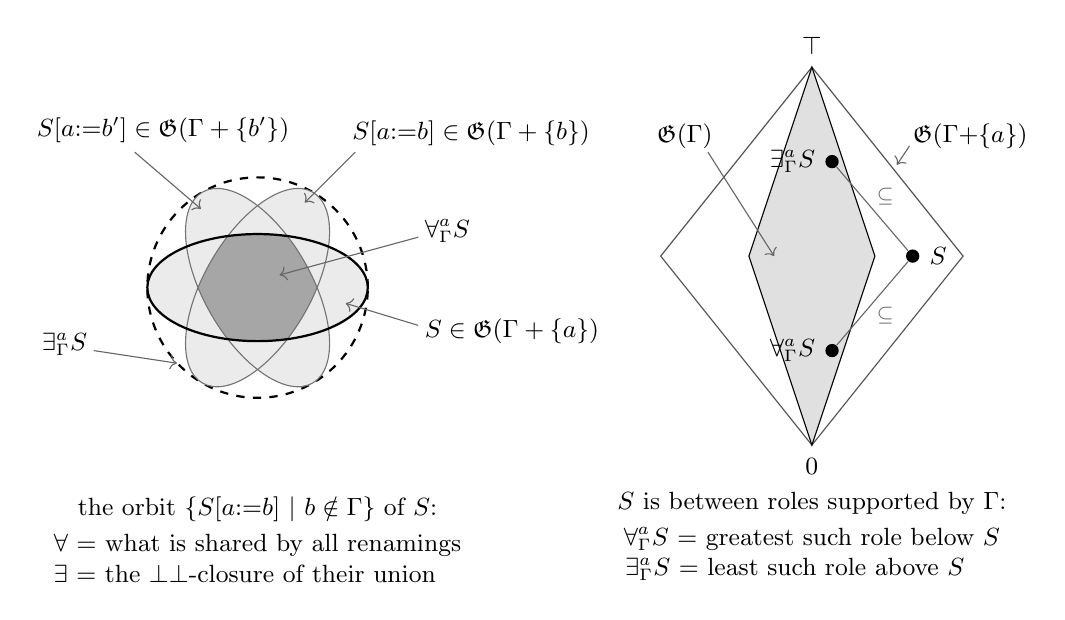
\begin{tikzpicture}[scale=0.8, every node/.style={font=\small}]

% ---------- left panel: the orbit picture ----------
\begin{scope}[yshift=-5mm]
  % exists: dashed bot-bot-closed envelope of the union
  \draw[dashed, black, thick] (0,0) circle (1.75);
  % union of the renamed copies, filled lightly
  \foreach \r in {0,60,120} \fill[black!8, rotate=\r] (0,0) ellipse (1.75 and 0.85);
  % forall: intersection of all copies, filled darkly
  \begin{scope}
    \clip (0,0) ellipse (1.75 and 0.85);
    \clip[rotate=60] (0,0) ellipse (1.75 and 0.85);
    \fill[black!35, rotate=120] (0,0) ellipse (1.75 and 0.85);
  \end{scope}
  % outlines; the 0-degree copy is S itself (thick)
  \foreach \r in {60,120} \draw[black!55, rotate=\r] (0,0) ellipse (1.75 and 0.85);
  \draw[thick] (0,0) ellipse (1.75 and 0.85);
  % labels for the copies
  \node[right] at (2.5,-0.7) {$S \in \G(\Gamma+\{a\})$};
  \draw[->, black!60] (2.55,-0.6) -- (1.4,-0.25);
  \node[above right] at (1.35,2.1) {$S[a{:=}b] \in \G(\Gamma+\{b\})$};
  \draw[->, black!60] (1.55,2.15) -- (0.75,1.35);
  \node at (-1.5,2.5) {$S[a{:=}b'] \in \G(\Gamma+\{b'\})$};
  \draw[->, black!60] (-1.95,2.15) -- (-0.9,1.25);
  % labels for the two operations
  \node[right, align=left] at (2.5,0.9) {$\forall^a_\Gamma S$};
  \draw[->, black!60] (2.55,0.8) -- (0.35,0.2);
  \node[left, align=right] at (-2.55,-0.9) {$\exists^a_\Gamma S$};
  \draw[->, black!60] (-2.6,-1.0) -- (-1.28,-1.2);
  % explanation
  \node[align=center] at (0,-4)
    {the orbit $\{S[a{:=}b]\ |\ b \notin \Gamma\}$ of $S$:\\[2pt]
     $\forall$ = what is shared by all renamings\\
     $\exists$ = the $\bot\bot$-closure of their union\ \ \ \ };
\end{scope}

% ---------- right panel: the sandwich in the lattice ----------
\begin{scope}[xshift=88mm]
  % ambient lattice of roles over Gamma + {a}
  \draw[black!70] (0,3) -- (2.4,0) -- (0,-3) -- (-2.4,0) -- cycle;
  \node[above] at (0,3.05) {$\top$};
  \node[below] at (0,-3.05) {$0$};
  \node[above right] at (1.45,1.55) {$\G(\Gamma{+}\{a\})$};
  \draw[->, black!60] (1.55,1.75) -- (1.35,1.45);
  % sublattice of a-independent roles
  \fill[black!12] (0,3) -- (1.0,0) -- (0,-3) -- (-1.0,0) -- cycle;
  \draw[black] (0,3) -- (1.0,0) -- (0,-3) -- (-1.0,0) -- cycle;
  \node[above left] at (-1.42,1.55) {$\G(\Gamma)$};
  \draw[->, black!60] (-1.65,1.65) -- (-.6,0);
  % S and its two best a-independent approximations
  \node[circle, fill=black, inner sep=1.7pt, label=right:{$S$}] (S) at (1.6,0) {};
  \node[circle, fill=black, inner sep=1.7pt, label=left:{$\forall^a_\Gamma S$}] (all) at (0.32,-1.5) {};
  \node[circle, fill=black, inner sep=1.7pt, label=left:{$\exists^a_\Gamma S$}] (ex) at (0.32,1.5) {};
  \draw[black!60] (all) -- (S) node[midway, below right=-2pt] {\scriptsize$\subseteq$};
  \draw[black!60] (S) -- (ex) node[midway, above right=-2pt] {\scriptsize$\subseteq$};
  % explanation
  \node[align=center] at (0,-4.45)
    {$S$ is between roles supported by $\Gamma$:\\[2pt]
     $\forall^a_\Gamma S$ = greatest such role below $S$\\
     $\exists^a_\Gamma S$ = least such role above $S\ \ \ \ $};
\end{scope}
\end{tikzpicture}
\caption{Visualizing $\forall^a_\Gamma,\exists^a_\Gamma\colon \G(\Gamma+\{a\})\to\G(\Gamma)$ on a role $S$ with free variables $\Gamma+\{a\}$. Left: substituting each fresh name $b\notin\Gamma$ for $a$ yields the orbit of renamed copies of $S$; $\forall^a_\Gamma S$ is their intersection, while $\exists^a_\Gamma S$ is the $\bot\bot$-closure of their union (the dashed envelope, which may properly round out the union). Both are invariant under all renamings of $a$, hence supported by $\Gamma$ alone. Right: order-theoretically, these are the two best approximations of $S$ by $a$-independent roles, i.e.\ the adjoints sandwiching the inclusion $\G(\Gamma)\hookrightarrow\G(\Gamma+\{a\})$.}
\label{fig:rolequantifiers}
\end{figure}


We extend propositional connectives of \cref{tab:connectives}, with two new ones. First, let $\bbrack{\phi(\Gamma;\Delta)}_{\Gamma+\Delta}$ have $\texttt{p}$ as a premisory role and $\texttt{c}$ as a conclusory role.

$$\bbrack{\forall \Delta\colon \phi(\Gamma;\Delta)}_{\Gamma}:=\langle \forall^\Delta_\Gamma(\texttt{p}),\ \exists^\Delta_\Gamma(\texttt{c}) \rangle \qquad \bbrack{\exists \Delta\colon \phi(\Gamma;\Delta)} := \bbrack{\neg \forall \Delta\colon \neg \phi(\Gamma;\Delta)}$$


\lemmawithproof{prop:conservativity}{
    Let $s:=\sum_{i \in \bar n} a^+_i + \sum_{j \in \bar m} b^-_j \in M(\Gamma)$, where $\Gamma=\Delta+\Theta$. The formula $F_\Theta = \forall \Theta\colon (a_1 \otimes ... \otimes a_n)\multimap (b_1 \parr ... \parr b_m)$ is a theorem (in context $\Delta$) of a nominal frame $\cX := (X, I)$ iff the $\Delta$ orbit of $a_1,...,a_n\vdash_\Delta b_1,...,b_m$ lies in $I$.
    Consequently, $\eta$ is conservative.
}{

   Theoremhood is tantamount to $\bbrack{F_\Theta}^-\subseteq I$. Unpacking the expression:

   \begin{align*}
    \bbrack{F_\Theta}^- &\subseteq I&& \text{Defn of }\vDash\\ 
    \bbrack{\forall \Theta\colon \neg(\bigotimes_i a_i)\parr ({\large{\underset{j}{\parr}}} b_j)}^- &\subseteq I&& \text{Defn of }\multimap\\ 
    \bbrack{\forall \Theta\colon ({\large{\underset{i}{\parr}}} \neg a_i)\parr ({\large{\underset{j}{\parr}}} b_j)}^- &\subseteq I&& \text{DeMorgan duals: }\otimes,\parr \\ 
    \exists^\Theta_\Delta\bigl(\bbrack{({\large{\underset{i}{\parr}}} \neg a_i)\parr ({\large{\underset{j}{\parr}}} b_j)}^-\bigr) &\subseteq I&& \text{Conclusory semantic role for }\forall\\ 
    \exists^\Theta_\Delta\bigl(\bigotimes_i a^{+\bot\bot}_i \otimes \bigotimes_j b^{-\bot\bot}_j\bigr) &\subseteq I&& \text{Conclusory semantic role for }\parr\\ 
    \bigvee_{\pi \in G_\Delta} \pi\bigl(\bigotimes_i a^{+\bot\bot}_i \otimes \bigotimes_j b^{-\bot\bot}_j\bigr) &\subseteq I&& \text{Defn of }\exists^\Theta_\Delta\\ 
    \forall \pi \in G_\Delta\colon \pi\bigl(\bigotimes_i a^{+\bot\bot}_i \otimes \bigotimes_j b^{-\bot\bot}_j\bigr) &\subseteq I&& \text{Universal property of joins}\\
   \bigl(\textstyle\bigcup_{\pi\in G_\Delta}\pi\{s\}\bigr)^{II} &\subseteq I
     && (-\otimes-)=(-{+}-)^{II},\ \textstyle\sum_i\{a_i^+\}{+}\sum_j\{b_j^-\}=\{s\};\\ &&&\ \pi\,\text{commutes with }(-)^{II}\\
  \bigl(\langle s\rangle_\Delta\bigr)^{II} &\subseteq I
     && \langle s\rangle_\Delta:=\bigcup_{\pi\in G_\Delta}\pi\{s\}=\{s\}_\Delta\ (\Delta\text{-orbit})\\
   \langle s\rangle_\Delta &\subseteq I
     && I=I^{\bot\bot}, (-)^{II}\text{ expansive, so }Y^{II}\subseteq I\iff Y\subseteq I\\
   a_1,\dots,a_n &\vdash_\Delta b_1,\dots,b_m
     && \langle s\rangle_\Delta\subseteq I\ \text{is goodness of the sequent }(\Delta\text{ fixed})   
    \end{align*}
    
    Conservativity of $\eta$ is a special case where we let $\Delta\mapsto \Gamma$ and $\Theta\mapsto \varnothing$.
}


\subsection{A desirable structural property}

A {\it hyperdoctrine} is a category-theoretic concept which allows one to talk very generally about the contexts in which one can interpret predicate logic.

\begin{proposition}
\label{prop:hyper}
The nominal set $\G_{\F_X}$ for the frame $(X,I)$ is a MALL hyperdoctrine {\it without} Beck-Chevalley, which is satisfied iff $I$ is substitution-equivariant (\cref{def:substeq}).
\end{proposition}

This is proven in \cref{sec:hyper}, and we define substitution-equivariance directly below.
We would like to talk about $\cat{Nom}$ subobjects which are closed under substitution, but nominal sets do not have a built-in notion of substitution. 
However, the subobjects of a $\cat{Nom}$ monoid do have such a notion.

\begin{definition}
\label{def:substeq}
A {\it substitution}-equivariant subobject of a monoid in $\cat{Nom}$, $A \rightarrowtail M$, is one which is closed under identifying names in the following sense. 
Suppose $\{a,b\}\subseteq \Gamma$ with $\tau$ being the permutation that swaps $a$ and $b$, and let $w_1 \in M(\Gamma\setminus\{a\})$ and $w_2 \in M(\Gamma\setminus\{b\})$ and $w_1+w_2 \in A(\Gamma)$. 
Substitution-equivariance means that $w_1 +\tau(w_2) \in A(\Gamma\setminus\{a\})$.
\end{definition}

For example, consider $\N[y1]$, i.e. $\Gamma$ is sent to multisets of elements of $\Gamma$ which we'll depict as lists. Let $A\rightarrowtail \N[y1]$ pick out all multisets that mention some $a \in \Gamma$ at least twice, and let $B$ have the opposite condition (so $\N[y1]\cong A+B$). $A$ is substitution equivariant, e.g. suppose we express $[a,a,b,c]\in A(\{a,b,c\})$ as $[a,b]+[a,c]$. We use the isomorphism swapping $b$ and $c$ and check if $[a,a,b,b] \in A(\{a,b\})$, which it is. Conversely, $B$ is not substitution equivariant: $[a,b,c] \in B(\{a,b,c\})$ and can be decomposed as $[a,b]+[c]$, but if we apply the isomorphism and add we get $[a,b,b]$ which is not in $B(\{a,b\})$. 

We could consider working in a category $\Nom$ but instead allows us to substitute variables rather than the analogous subcategory of $[\FF,\Set]$ (called ${\cat{Ren}}$ for `renaming' in \cite{lenke2026unified}), is that this would structurally bake in the assumption that $P(a,c),H(b,c)\vdash O(b,c)$ generically implies $P(a,c),H(a,c)\vdash O(a,c)$. 
This is too much, e.g. `$a$ perpetrated crime $c$', `$b$ was harmed in crime $c$', `$b$ is owed something for crime $c$'. Another example comes from Robert's Rules of Order: $Motion(a,m),Second(b,m)\vdash Considered(m)$ is a good inference ($a$'s motion must be seconded for the motion to be considered) yet we don't want to be structurally  forced into $Motion(a,m),Second(a,m)\vdash Considered(m)$ due to the substitution $[b\mapsto a]$. In general, any language with an inequality predicate must not be invariant (in {\it general}) with respect to substitutions of non-free variables.


Consider the following sequent rules: 


\vspace{0mm}
\begin{center}
\boxed{
\RightLabel{$\forall$L}
\AxiomC{$\cA, P\vdash_{\Gamma +\{x\}} \cB$}
\UnaryInfC{$\cA,\forall x.P \vdash_{\Gamma} \cB$}
\DisplayProof}
\hspace{8mm}
\boxed{
\doubleLine
\RightLabel{$\forall$R}
\AxiomC{$\cA \vdash_{\Gamma+\{x\}} P,\cB$}
\UnaryInfC{$\cA\vdash_{\Gamma}\forall x.P, \cB$}
\DisplayProof}
\end{center}
\vspace{0mm}

\lemmawithproof{lemma:quantrules}{
    Let $\cX:=(X,I)$ be a nominal frame that is substitution-equivariant. The above $\forall$L and $\forall$R rules are satisfied in the semantic frame $\hat \cX$.
}{
Let $\iota$ be the action of $\G_{\F_X}$ on $\Gamma\hookrightarrow \Gamma+\Delta$. 
Let $S \in \G_{\F_X}(\Gamma)$ (representing the arbitrary background semantic value $\bbrack{\cA\multimap \cB}$) and $T \in \G_{\F_X}(\Gamma+\Delta)$ represent the premisory semantic value of $P$. 
We will deploy Beck-Chevalley at the outset because our formulas in $\cA$ and $\cB$ might contain quantifiers, and to lift those to context $\Gamma+\Delta$ (via $\iota(S)$) Beck-Chevalley is precisely what is needed. We now first show the $\forall$L rule: 

\begin{align*}
&\iota(S) \otimes  T \subseteq \iota(I)  && \text{Semantic consequence relation}\\
&\implies \iota(S) \otimes  \iota(\forall^\Delta_\Gamma T) \subseteq \iota(I)   &&\text{Adjunction counit: }\forall^\Delta_\Gamma\cdot \iota \leq  \id_{\G_{\F_X}(\Gamma+\Delta)} \\
&\iff \iota(S \otimes \forall^\Delta_\Gamma T) \subseteq \iota(I)   &&\iota \text{ preserves quantale structure}\\
&\iff S \otimes \forall^\Delta_\Gamma T \subseteq I && \iota \text{ is an inclusion}\\
\end{align*}

Now let $T$ represent the conclusory semantic value of $P$.

\begin{align*}
&\iota(S) \otimes  T \subseteq \iota(I)  && \text{Semantic consequence relation}\\
&\iff  \exists^\Delta_\Gamma(\iota(S)\otimes T) \subseteq I && \exists^\Delta_\Gamma \dashv \iota \text{ adjunction}\\
&\iff S \otimes \exists^\Delta_\Gamma T \subseteq I  && \text{Frobenius reciprocity (\cref{lemma:frob})}\\
\end{align*}
}


\section{Finite computation}
\label{sec:fin}

As we mentioned in \cref{sec:rel}, it is nice to represent a nominal set via a signature which has finite data. Although a nominal set morphism is a function between infinite sets, we can use the fact that morphisms must be equivariant and give data per orbit (which means one piece of data per predicate symbol).\footnote{This also arises from the adjunction described in \cref{sec:species} between a category of signatures and $\Nom$}


Using adjunctions we can represent morphisms which would normally require infinite data with finite data. For example, $\Nom$ morphisms $\Sigma \to X$ out of a nominal set presented by a signature (\cref{def:sig}), $\Mon \Nom$ morphisms $\N[\Sigma]\to(X,\mu,e)$, and ${\rm Quant}\ \Nom$ morphisms $\cP(\N[\Sigma]) \to (X,\bigvee,\otimes)$, are all expressed by picking an element of $X$ for every generator in $\Sigma$.


We now define some more operations on subobjects of internal quantales. Subtraction $a-s$ of elements of $\N[X]$ is partial, defined when $a\geq s$.\footnote{Here we invoke the fact that this is the free quantale on a {\it free} monoid, since this guarantees that the monoid is cancellative such that the partial $-$ operation is well-defined.} We reserve $\setminus$ for ordinary set difference; the operation $\{a-s\ |\ a\in A,\ a\geq s\}$ on a subobject $A$ is written $\{s\}\multimap A$, which is what it is. There is also a truncated subtraction operation $A\monus s:=\{x\mapsto \max(0,\ a(x)-s(x))\ |\ a \in A\}$.


\begin{definition}
    \label{def:orbitfinite}
    An {\it orbit-finite} subobject of $\delta^\Delta M$ is one presented
    by a finite list $g_1,\dots,g_m$ of elements of $M$ as
    $A\ =\ \bigcup_{i=1}^{m}G_\Delta\bullet g_i$
    i.e.\ every element of $A$ is obtained from some $g_i$ by injectively
    renaming its names outside $\Delta$ to names outside $\Delta$. A
    $\Delta$-supported subset of $M$ admits such a presentation iff it has
    finitely many $G_\Delta$-orbits.
\end{definition}

Enlarging the context refines orbits: a $G_\Gamma$-orbit splits into finitely many $G_{\Gamma+\Delta}$-orbits, indexed by how the fresh names of a representative meet $\Delta$. This is used throughout to move presentations between contexts.

\begin{lemma}
    \label{lemma:orbitrefine}
    Let $A=\bigcup^m_{i=1} G_{\Gamma+\Delta}\bullet g_i$ be an orbit-finite subobject of $\delta^{\Gamma+\Delta} M$. 
    The `unfreeze' operation is $G_\Gamma\bullet A=\bigcup^m_{i=1} G_\Gamma\bullet g_i$, a subobject of $\delta^{\Gamma}M$ with the same generators $g_i$. This will in general only add elements, as $G_{\Gamma+\Delta }\leq G_\Gamma$. If we would like to re-express this larger subset as an  orbit-finite subobject of $\delta^{\Gamma+\Delta} M$, we have to add new generators.  
    For $g\in M$ and a partial injection
    $\alpha\colon\supp(g)\setminus\Gamma\prightarrowtail\Delta$, write
    $\alpha\,g$ for the joint substitution applying $\alpha$ and moving the names on which $\alpha$ is undefined to fresh names. 
    Then $G_\Gamma\bullet A$ is presented by an orbit-finite subobject of $\delta^{\Gamma+\Delta} M$ whose generators are $\{\alpha g_i\ |\ 1 \leq i \leq m,\ \alpha\colon {\supp(g)\setminus\Gamma\prightarrowtail\Delta}\}$. We can moreover identify which orbit a given $\pi g$ lives in, for some $\pi \in G_\Gamma$, as there is a unique $\alpha_\pi$ which agrees with $\pi$.
\end{lemma}
\begin{proof}
Since $G_{\Gamma+\Delta}\subseteq G_\Gamma$, we have
$G_\Gamma\bullet A=\bigcup_i G_\Gamma\bullet G_{\Gamma+\Delta}\bullet g_i
=\bigcup_i G_\Gamma\bullet g_i$, a finite union of $G_\Gamma$-orbits,
invariant under $G_\Gamma$ and hence $\Gamma$-supported.
 
Let $\pi \in G_\Gamma$. For $a\notin\Gamma$ we have
$\pi(a)\notin\Gamma$, so either $\pi(a)\in\Delta$ or
$\pi(a)\notin\Gamma+\Delta$: thus $\alpha_\pi$ records exactly which names
of $g$ the permutation $\pi$ sends into $\Delta$, and where. Fix $\pi$ and
put $\alpha:=\alpha_\pi$; realize $\alpha\,g$ as $\pi_\alpha g$, where
$\pi_\alpha\in G_\Gamma$ maps $\mathrm{dom}(\alpha)$ by $\alpha$ and the
remaining names of $\supp(g)\setminus\Gamma$ to fresh names outside
$\Gamma\cup\Delta\cup\supp(g)$. On $\mathrm{dom}(\alpha)$ the maps $\pi$
and $\pi_\alpha$ agree; on the remaining names of
$\supp(g)\setminus\Gamma$ both take values outside $\Gamma+\Delta$, so the
injection $\pi_\alpha a\mapsto\pi a$ lives on names outside
$\Gamma+\Delta$ and extends to some $\sigma\in G_{\Gamma+\Delta}$ with
$\sigma\pi_\alpha a=\pi a$ for all $a\in\supp(g)\setminus\Gamma$, hence
for all $a\in\supp(g)$ (all three maps fix $\Gamma$ pointwise); therefore
$\pi g=\sigma(\alpha\,g)\in G_{\Gamma+\Delta}\bullet(\alpha\,g)$. (The
same argument, applied to two choices of fresh names, shows the orbit
$G_{\Gamma+\Delta}\bullet(\alpha\,g)$ does not depend on the choice.)
 
For the generator list: each element of $G_\Gamma\bullet A$ is $\pi g_i$
for some $i$ and $\pi\in G_\Gamma$, hence lies in
$G_{\Gamma+\Delta}\bullet(\alpha_{\pi}\,g_i)$ by the classification;
conversely $\alpha\,g_i=\pi_\alpha g_i\in G_\Gamma\bullet g_i$ and
$G_{\Gamma+\Delta}\subseteq G_\Gamma$, so each listed orbit is contained
in $G_\Gamma\bullet A$. For each $i$ there are
a finite number of
partial injections.
\end{proof}


\begin{definition}
    Let $\cW(-)\colon \Sub Q \to \Sub Q$ be the {\it monotonic weakening}, sending $A\rightarrowtail Q$ to $\cW(A):= A \otimes \top$, where $Q$ itself is the top element $\top$ of its subobject lattice. When $Q=\cP M$, we implicitly interpret $\cW(m\in M)$ as $\cW(\{m\})$.
\end{definition}

$\cW$ is a closure operator. For example, $\cW(A\vdash_\Gamma B)$ represents sequents $Z_+, A\vdash_\Gamma B, Z_-$ for all $Z_+,Z_-$ multisets of ${N}(\Gamma)$ elements. 

\subsection{In progress: Constructible triples: adding reflexive weakening}
\label{sec:constructibletriple}


\begin{definition}
    \label{def:reflweak}
    The {\it reflexive submonoid} $R \rightarrowtail \N[X]^2$ consists of the elements with $s^+ = s^-$ (as multisets on $X$): the sequents with one and the same arbitrary multiset on both sides.
    Let $\cR(-)\colon \Sub Q \to \Sub Q$ be the {\it reflexive weakening}, sending $A \rightarrowtail Q$ to $\cR(A):=A\otimes R$. As with $\cW$, we implicitly interpret $\cR(m \in M)$ as $\cR(\{m\})$.
\end{definition}

For example, $\cR(A\vdash_\Gamma B)$ represents the sequents $Z,A\vdash_\Gamma B,Z$ for all multisets $Z$ of $N(\Gamma)$ elements.
Two further gadgets will be used repeatedly. First, any $s \in M$ is has a greatest lower and least upper bound in $R$. The least upper bound is {\it least reflexive dominator} of $s \in M$ is $\hat s := (s^+\vee s^-)^+ + (s^+\vee s^-)^- \in R$, where $\vee$ is the pointwise maximum of multisets on $X$. The greatest lower bound is denoted $s_r:=\sum_y \min(s(y^+),s(y^-))\,(y^++y^-)$. Every $s$ decomposes canonically as $s = s_c + s_r$ with the {\it core} being $s_c:=s-s_r$. The {\it imbalance} of $s$ is the $\Z$-valued multiset $\imb(s):=s^+ - s^-$ on $X$; note that $|\imb(s)|:=\sum_y |\imb(s)(y)|$ is equal to $|s_c|$. 

\begin{lemma}
    \label{lemma:reflprops}
    Some properties of $\cR$:
    \begin{itemize}
        \item ({\bf a}) $\cR$ is a closure operator on $\Sub Q$ preserving unions, and it commutes with the permutation action: $\pi\,\cR(A)=\cR(\pi A)$.
        \item  ({\bf b}) $\cR \leq \cW$, and $\cW\cdot\cR = \cR\cdot\cW = \cW$.
        \item ({\bf c}) For $\rho \in R$: $\rho \geq s \iff \rho \geq \hat s$, and in that case $\rho - \hat s \in R$.
        \item  ({\bf d}) $\imb$ is additive, $\imb(\pi s)=\pi\,\imb(s)$, and $\imb(s)=0 \iff s \in R$. Consequently $t \in \cR(m) \iff m \leq t$ and $\imb(t)=\imb(m)$ (which we denote $m\leq_\cR t$).
        \item ({\bf e}) For $l,m\in M$ and $\rho\in R$, $m+\rho\geq l \iff \rho\geq\widehat{l\monus m}$, and in that case $\rho-\widehat{l\monus m}\in R$. So $\widehat{l\monus m}$ is the least reflexive element which, added to $m$, reaches above $l$; taking $m=0$ recovers ({\bf c}).
    \end{itemize}
\end{lemma}
\begin{proof}
({\bf a}) $0 \in R$ gives $A \subseteq \cR(A)$; $R$ is a submonoid containing $0$, so $R\otimes R=R$ and $\cR$ is idempotent; $\otimes$ distributes over unions. The action renames atoms pointwise and preserves signs, so $\pi(a+\rho)=\pi a+\pi\rho$ with $\pi\rho\in R$.

({\bf b}) $R\subseteq M=\top$ gives $\cR\leq\cW$; since $0\in R$, $R\otimes M=M$, so $\cW(\cR(A))=A\otimes R\otimes M=A\otimes M=\cW(A)$, and likewise in the other order.

({\bf c}) If $\rho=z^++z^-\geq s$ then $z\geq s^+$ and $z\geq s^-$, so $z\geq s^+\vee s^-$, i.e.\ $\rho\geq\hat s$; conversely $\hat s\geq s$. Then $\rho-\hat s=(z-(s^+\vee s^-))^++(z-(s^+\vee s^-))^-\in R$.

({\bf d}) Additivity and equivariance are immediate, and $\imb(s)=0$ says exactly $s^+=s^-$. If $t=m+\rho$ with $\rho\in R$ then $m\leq t$ and $\imb(t)=\imb(m)$; conversely if $m\leq t$ and $\imb(t)=\imb(m)$ then $\imb(t-m)=0$, i.e.\ $t-m\in R$.

({\bf e}) At each signed claimable $x$, $m(x)+\rho(x)\geq l(x)$ says $\rho(x)\geq l(x)-m(x)$, and as $\rho(x)\geq0$ this holds iff $\rho(x)\geq\max(0,l(x)-m(x))=(l\monus m)(x)$. So $m+\rho\geq l\iff\rho\geq l\monus m$, and ({\bf c}) applied to $s:=l\monus m$ turns the right-hand side into $\rho\geq\widehat{l\monus m}$ with $\rho-\widehat{l\monus m}\in R$. For $m=0$ we have $l\monus 0=l$, giving ({\bf c}) back.
\end{proof}


\begin{definition}
    \label{def:constructibletriple}
    A {\it constructible triple} presenting an element of $\cP(M)$ (equivalently a subobject of $\delta^\Delta(M)$) is a triple $\langle\kappa,\mu,\lambda\rangle$ of orbit-finite subobjects, interpreted as the subobject stratified as
    $$\bigl(\kappa\setminus(\cR(\mu)\cup\cW(\lambda))\bigr)\ \sqcup\ \bigl(\cR(\mu)\setminus\cW(\lambda)\bigr)\ \sqcup\ \cW(\lambda).$$
    As a set, this is $\kappa\cup\cR(\mu)\cup\cW(\lambda)$, so every computation below may be carried out with plain unions; the point of the stratified reading is that its three parts are disjoint. 
\end{definition}

\begin{lemma}[Deciding membership]
    \label{lemma:matching}
    Let $\kappa,\lambda,\mu$ be orbit-finite subobjects of $\delta^\Delta M$ and $t\in M$ a concrete element. 
    Then the memberships $t\in\kappa$, $t\in\cW(\lambda)$ and $t\in\cR(\mu)$ are decidable.
\end{lemma}
\begin{proof}
    Write a generator list for an orbit-finite $A\rightarrowtail\delta^\Delta M$ as $A=\bigcup_iG_\Delta\bullet g_i$ (\cref{def:orbitfinite}). 
    A permutation $\pi\in G_\Delta$ with $\pi g_i=t$ is determined on $\supp(g_i)$ and must carry $\supp(g_i)\setminus\Delta$ injectively into $\supp(t)\setminus\Delta$, so there are finitely many candidates to test and $t\in\kappa$ is decidable. 
    For $\cW$: $t\in\cW(\lambda)$ iff $l\leq t$ for some $l\in\lambda$, and $l\leq t$ forces $\supp(l)\subseteq\supp(t)$; 
    the elements of $\lambda$ so supported are, by the same count, finitely many and effectively listable, so the condition is decidable. 
    For $\cR$: by \cref{lemma:reflprops}~{\bf d}, $t\in\cR(\mu)$ iff some $m\in\mu$ has $m\leq t$ and $\imb(m)=\imb(t)$, which is the previous search with one further equality test.
\end{proof}


\begin{lemma}
    \label{lemma:tripleintersectbin}
    By distributing the intersection over the unions, there are nine terms to the intersection of two computable triples as follows: 
    \begin{center}
    \begin{tabular}{||c||c|c|c||}
        \hline
        $\cap$ & $\kappa_2$ & $\cR(\mu_2)$ & $\cW(\lambda_2)$\\
        \hline\hline
        $\kappa_1$ & $\kappa_1\cap \kappa_2$ & $\kappa_1\cap \cR(\mu_2)$  & $\kappa_1\cap \cW(\lambda_2)$ \\
        \hline
        $\cR(\mu_1)$ & $\kappa_2\cap \cR(\mu_1)$ & $\cR(m_1\vee m_2\ |\ (m_1,m_2)\in \mu_1 \times_{\Z[X]} \mu_2)$ & $\cR(m_1 + \widehat{l_2\monus m_1}\ |\ (m_1,l_2)\in \mu_1 \times \lambda_2)$ \\
        \hline
        $\cW(\lambda_1)$ & $\kappa_2\cap \cW(\lambda_1)$ & $\cR(m_2 + \widehat{l_1\monus m_2}\ |\ (l_1,m_2)\in \lambda_1 \times \mu_2)$ & $\cW(l_1\vee l_2\ |\ (l_1,l_2)\in \lambda_1 \times \lambda_2)$ \\
        \hline
    \end{tabular}
    \end{center}

    Note that $\vee$ is join in the $\leq$ order (so pointwise maximum for multiset counts). We denote the pullback in set $-\times_{\Z[X]} -$ to implicitly use the $\imb(-)\colon M \to \Z[X]$ function, so this gives all pairs which agree on their imbalance. And recall that $\widehat{(-)}$ is the {\it least reflexive dominator} operation.
    
\end{lemma}
\begin{proof}

    The five cells in the $\kappa$ rows and columns are filterings of elements of $\kappa_1$ and $\kappa_2$, computable by \cref{lemma:matching}. The diagonal cells are also evidently the intersection of the implicit infinite sets. We now explain the formula for computing the intersection of $\cW(l)=\{lA^+B^-\ |\ A,B\in \N[X]\}$ and $\cR(m)=\{mC^+C^-\ |\ C \in \N[X]\}$. First, if $l\leq m$, then $\cR(m)\subseteq \cW(l)$ and their intersection is $\cR(m)$: this corresponds to the fact that the truncated subtraction is empty. If $\cR(m)$ gets smaller via intersection, it is because it has been shifted by some $C^+C^-$ factor. The smallest factor which can be added to $m$ to reach something above $l$ is $\widehat{l\monus m}$ (\cref{lemma:reflprops}~{\bf e}).
\end{proof}


\begin{lemma}
    \label{lemma:reflresidual}
   For a constructible triple $\langle \kappa, \mu, \lambda \rangle = C \rightarrowtail \delta^\Delta M$ and any $s\in M$ with $\supp(s)\subseteq\Delta$, the subobject $\{s\}\multimap C \rightarrowtail \delta^\Delta M$ is also a constructible triple $\langle \kappa', \mu', \lambda' \rangle$ with $\kappa' = \{s\}\multimap \kappa$, $\mu' = \{m+\widehat{s\monus m}-s\ |\ m \in \mu\}$, and $\lambda' =\lambda\monus s$.
\end{lemma}
\begin{proof}

We start by expressing $\{s\}\multimap C$ as $(\{s\}\multimap \kappa) \cup (\{s\}\multimap \cR(\mu)) \cup (\{s\}\multimap \cW(\lambda))$.
The simplified form of $\mu'$ comes from \cref{lemma:reflprops}({\bf e}). $s+t\geq l$ iff $t(x)\geq l(x)-s(x)$ at every signed claimable $x$, i.e.\ iff $t\geq l\monus s$, so $\{s\}\multimap\cW(\lambda)=\cW(\lambda\monus s)$.
It remains to see that $\kappa'$, $\mu'$ and $\lambda'$ are orbit-finite (\cref{def:orbitfinite}). Since $\supp(s)\subseteq\Delta$, every $\pi\in G_\Delta$ fixes $s$, so $\pi(\{s\}\multimap A)=\{\pi s\}\multimap\pi A=\{s\}\multimap\pi A$; and $\{s\}\multimap(-)$ preserves unions, being a preimage. Hence $\{s\}\multimap(G_\Delta\bullet A)=G_\Delta\bullet(\{s\}\multimap A)$. Applying this to the generators of $\kappa$, $\cW(\lambda)$ and $\cR(\mu)$ --- using $\pi\cW(A)=\cW(\pi A)$ and $\pi\cR(A)=\cR(\pi A)$ (\cref{lemma:reflprops}~{\bf a}) to write those last two over generators --- the computations above turn each generator of $C$ into at most one generator of $\{s\}\multimap C$.
\end{proof}


The hypothesis $\supp(s)\subseteq\Delta$ costs no generality: $C$ may first be re-presented at the enlarged context $\Delta+(\supp(s)\setminus\Delta)$ (\cref{lemma:orbitrefine}), which renames generators and so changes neither their sizes nor their imbalances.

The residuals of $\cW$- and $\cR$-orbits reduce by currying to two ``unit'' computations, generalizing $0=\top\multimap\bot$: for any constructible $C$,
$\cW(s)\multimap C=\{s\}\multimap(\top\multimap C)$ (since $\cW(s)=\{s\}\otimes\top$) and $\qquad \cR(s)\multimap C=\{s\}\multimap(R\multimap C)$ (since $\cR(s)=\{s\}\otimes R$). 


\noindent\rule{\textwidth}{1pt}

\subsection{Unchecked content}


Decidability of the conditions ``$\cW(k)\subseteq C$'' and ``$\cR(k)\subseteq C$'' (of which the first defines $\kappa_0$ below) reduces, via \cref{lemma:reflresidual}, to the following covering test, since $\cW(z)\subseteq C\iff M=\{z\}\multimap C$ and $\cR(z)\subseteq C\iff R\subseteq\{z\}\multimap C$.

\begin{lemma}
    \label{lemma:covertest}
    Let $E=\kappa'\cup\cW(\lambda')\cup\cR(\mu')$ be a constructible triple at a context $\Gamma$, with maximal sizes $s_{\kappa'},s_{\lambda'},s_{\mu'}$, and let $\beta:=\max_{w\in\mu'}|\imb(w)|$ (zero if empty) and $B_2:=\beta+2s_{\kappa'}+2$. Then:
    \begin{enumerate}
        \item[({\bf i})] $M=E$ iff no $t$ with $|t|\leq B_2$ avoids $E$;
        \item[({\bf ii})] $R\subseteq E$ iff no {\it reflexive} $t$ with $|t|\leq B_2$ avoids $E$.
    \end{enumerate}
    Since elements of bounded size have bounded support, both conditions are decided by testing the finitely many candidate orbits, each test being that of \cref{lemma:matching}.
\end{lemma}
\begin{proof}
    Only the forward directions need proof: given any $t\notin E$, we produce $t'\notin E$ with $|t'|\leq B_2$. Note that avoidance of $\cW(\lambda')$ is inherited downward (its complement is down-closed), as is avoidance of each ``domination half'' of $\cR(w)$: if no renamed copy of $w$ lies below $t$, then none lies below any $t'\leq t$.

    {\it Case} $|\imb(t)|>\beta$: take $t'\leq t_c$ consisting of $\max(\beta,s_{\kappa'})+1$ core elements if $|\imb(t)|>\max(\beta,s_{\kappa'})$; otherwise take all of $t_c$ and pad with balanced pairs from $t_r$ until $|t'|>s_{\kappa'}$, which is possible unless $t$ has too little material, i.e.\ unless $|t|\leq s_{\kappa'}$, in which case $t$ itself serves as $t'$. In the two padding constructions $t'\leq t$, so $t'\notin\cW(\lambda')$; $|t'|>s_{\kappa'}$, so $t'\notin\kappa'$; and $|\imb(t')|>\beta$ (in the first construction because core elements contribute their full size to the imbalance; in the second because $\imb(t')=\imb(t)$), so $t'\notin\cR(w)$ for every $w$, by \cref{lemma:reflprops}~{\bf d}.

    {\it Case} $|\imb(t)|\leq\beta$: take $t':=t_c$ padded with balanced pairs from $t_r$ until $|t'|>s_{\kappa'}$ (if $t$ has too little material, $|t|\leq\beta+s_{\kappa'}+2$ and $t$ itself serves). Then $t'\leq t$ and $\imb(t')=\imb(t)$. As before $t'\notin\kappa'\cup\cW(\lambda')$. For each renamed copy $w$ of an element of $\mu'$: if $\imb(w)\neq\imb(t)$ then $t'\notin\cR(w)$ by the imbalance test; if $\imb(w)=\imb(t)$, then $t\notin\cR(w)$ forces $w\not\leq t$, hence $w\not\leq t'$, and again $t'\notin\cR(w)$.

    In both cases $|t'|\leq\beta+2s_{\kappa'}+2$. For ({\bf ii}), an avoiding $t\in R$ has $\imb(t)=0$, so only the second case arises and its construction stays inside $R$ (both $t_c=0$ and balanced pairs are reflexive).
\end{proof}


\subsubsection*{The $\forall$-intersection}

The intersection $\bigcap_{\pi\in G_\Gamma}\pi C$ at the heart of $\forall^\Delta_\Gamma$ has an elementwise reading: $t\in\bigcap_\pi\pi C$ iff $G_\Gamma\bullet t\subseteq C$. Its elements can be arbitrarily large, so the content of the theorem below is a {\it small-witness} bound: the $\cW$ and $\cR$ parts are generated by witnesses of bounded size. Since $\cR(\mu_C)$ is not upward closed, ``dominates a small witness'' is the wrong shape for the $\cR$ part; the right shape is ``differs from a small witness by a reflexive element''. The proof is a $q$-round game: a single fresh witness handles every renaming that keeps its names out of $\Delta$, and a renaming that instead pins one of them into $\Delta$ has spent one of the $q$ available names and is handled by the same argument one context larger.

\begin{lemma}
    \label{lemma:tripleintersect}
    Let $M:=\N[X]$ for an orbit-finite signed nominal set $X$, $r$ the maximal support size of elements of $X$. Fix a context $\Gamma$ and a finite set $\Delta$ of names disjoint from $\Gamma$, and let $C=\kappa_C\cup\cW(\lambda_C)\cup\cR(\mu_C)$ be a constructible triple subobject of $\delta^{\Gamma+\Delta}M$ with maximal sizes $s_\kappa,s_\lambda,s_\mu$. Let $q:=|\Delta|$, $s:=\max(s_\lambda,s_\mu)$, $N_\lambda:=s_\lambda(rs_\lambda q+1)^q$, $N_\cR:=s_\mu+2s(rsq+1)^q$, and fix a set $P$ of $r\max(s_\kappa,N_\lambda,N_\cR)$ names disjoint from $\Gamma$. Then
    $$\bigcap_{\pi\in G_\Gamma}\pi C\ =\ (G_\Gamma\bullet K)\ \cup\ \cW(G_\Gamma\bullet L)\ \cup\ \cR(G_\Gamma\bullet L_\cR)$$
    is a constructible triple subobject of $\delta^\Gamma M$, where
    \begin{align*}
    K&:=\{t\ |\ \supp(t)\subseteq\Gamma\cup P,\ |t|\leq s_\kappa,\ G_\Gamma\bullet t\subseteq C\},\\
    L&:=\{t\ |\ \supp(t)\subseteq\Gamma\cup P,\ |t|\leq N_\lambda,\ G_\Gamma\bullet t\subseteq\cW(\lambda_C)\},\\
    L_\cR&:=\{t\ |\ \supp(t)\subseteq\Gamma\cup P,\ |t|\leq N_\cR,\ G_\Gamma\bullet t\subseteq\cW(\lambda_C)\cup\cR(\mu_C)\}.
    \end{align*}
    These sets are computable: by \cref{lemma:orbitrefine}, an orbit condition $G_\Gamma\bullet t\subseteq S$ for $(\Gamma+\Delta)$-supported $S$ holds iff $\alpha\,t\in S$ for each of the finitely many partial injections $\alpha\colon\supp(t)\setminus\Gamma\prightarrowtail\Delta$, and each such membership is decided by \cref{lemma:matching}.
\end{lemma}
\begin{proof}
    Throughout, let $D_\lambda,D_\mu$ be orbit-finite subobjects of $\delta^{\Gamma+\Delta}M$ with maximal size $s_D$, and say $d\in D_\lambda\cup D_\mu$ {\em covers} $t$ {\em along} $\pi\in G_\Gamma$ if $d\leq\pi t$, and moreover $\imb(d)=\imb(\pi t)$ in case $d\in D_\mu$.

    {\it Small-witness claim: if $t$ is covered along every $\pi\in G_\Gamma$, then there is $w\leq t$ with $|w|\leq s_D(rs_Dq+1)^q$, covered along every $\pi\in G_\Gamma$ (side-conditions still relative to $\pi t$).} We induct on $q$, over all instances of the claim ($\Gamma$, $\Delta$ and $t$ vary along the way; $D_\lambda,D_\mu$ are fixed).

    If $q=0$ then $D_\lambda$ and $D_\mu$ are $G_\Gamma$-invariant. Take a cover $d_0\leq t$ along the identity and put $w:=d_0$. For any $\pi$, $\pi d_0\in D_\lambda\cup D_\mu$ lies in the same piece as $d_0$ and $\pi d_0\leq\pi w$; if $d_0\in D_\mu$ then $\imb(d_0)=\imb(t)$, so $\imb(\pi d_0)=\pi\,\imb(t)=\imb(\pi t)$ by equivariance of $\imb$ (\cref{lemma:reflprops}~{\bf d}).

    Let $q\geq1$. Choose $\pi_0\in G_\Gamma$ moving $\supp(t)\setminus\Gamma$ outside $\Gamma+\Delta$, take a cover $d_0\leq\pi_0t$ along $\pi_0$, and put $w_0:=\pi_0^{-1}d_0\leq t$, of size at most $s_D$, with at most $rs_D$ names outside $\Gamma$; if $d_0\in D_\mu$ then $\imb(w_0)=\pi_0^{-1}\imb(d_0)=\pi_0^{-1}\imb(\pi_0t)=\imb(t)$. For every $\pi\in G_\Gamma$ that moves $\supp(w_0)\setminus\Gamma$ outside $\Gamma+\Delta$: by \cref{lemma:orbitrefine}, $\pi w_0$ and $\pi_0w_0=d_0$ lie in the same fine $G_{\Gamma+\Delta}$-orbit, and $D_\lambda,D_\mu$ are each $G_{\Gamma+\Delta}$-invariant, so $\pi w_0\in D_\lambda\cup D_\mu$ lies in the same piece as $d_0$; and if that piece is $D_\mu$ then $\imb(\pi w_0)=\pi\,\imb(w_0)=\pi\,\imb(t)=\imb(\pi t)$. Every other $\pi$ pins some name $a\in\supp(w_0)\setminus\Gamma$ to some $z\in\Delta$, and the $\pi$ committing a given pin form a coset: for any fixed $\rho_{az}\in G_\Gamma$ with $\rho_{az}(a)=z$, $\{\pi\in G_\Gamma\ |\ \pi(a)=z\}=G_{\Gamma+z}\,\rho_{az}$, since $\pi(a)=z$ iff $\pi\rho_{az}^{-1}$ fixes $z$. For each of the at most $rs_Dq$ pairs $(a,z)$: the element $\rho_{az}t$ is covered along every $\sigma\in G_{\Gamma+z}$ (side-condition relative to $\imb(\sigma\rho_{az}t)$), which is the claim's hypothesis at context $\Gamma+z$ with name set $\Delta\setminus z$; by induction there is $w'_{az}\leq\rho_{az}t$ with $|w'_{az}|\leq s_D(rs_D(q{-}1)+1)^{q-1}$, covered along every $\sigma$. Put $w_{az}:=\rho_{az}^{-1}w'_{az}\leq t$ and $w:=w_0\vee\bigvee_{a,z}w_{az}$ (pointwise maximum), so $w\leq t$ and
    $$|w|\ \leq\ s_D+rs_Dq\cdot s_D(rs_D(q{-}1)+1)^{q-1}\ \leq\ s_D(rs_Dq+1)^{q}.$$
    Each $\pi\in G_\Gamma$ either satisfies $\pi w_0\leq\pi w$ with $\pi w_0\in D_\lambda\cup D_\mu$ as above, or, writing $\pi=\sigma\rho_{az}$, some $d\leq\sigma w'_{az}=\pi w_{az}\leq\pi w$ with side-condition relative to $\imb(\sigma\rho_{az}t)=\imb(\pi t)$; the side-conditions are stated relative to $\pi t$ throughout, so they are unaffected by taking the pointwise maximum. This proves the claim.

    {\it Recombination.} Put $U:=\{t\ |\ G_\Gamma\bullet t\subseteq\cW(\lambda_C)\cup\cR(\mu_C)\}$ and $U_\cW:=\{t\ |\ G_\Gamma\bullet t\subseteq\cW(\lambda_C)\}$. By \cref{lemma:reflprops}~{\bf d}, $t\in U$ iff $t$ is covered along every $\pi$ for $D_\lambda:=\lambda_C$, $D_\mu:=\mu_C$, and $t\in U_\cW$ iff so for $D_\lambda:=\lambda_C$, $D_\mu:=\varnothing$. Also $U$ is closed under adding reflexive elements, since $\pi(t+\rho)=\pi t+\pi\rho$ and both $\cW(\lambda_C)$ and $\cR(\mu_C)$ absorb them. We show: every $t\in U$ either dominates some $w\in U_\cW$ with $|w|\leq N_\lambda$, or is $t_0+\rho$ with $\rho\in R$, $t_0\in U$, $|t_0|\leq N_\cR$. If $t\in U_\cW$, the claim ($D_\mu=\varnothing$, $s_D=s_\lambda$) gives $w\leq t$ with $|w|\leq N_\lambda$ and $G_\Gamma\bullet w\subseteq\cW(\lambda_C)$. Otherwise $\pi_0t\in\cR(\mu_C)$ for some $\pi_0$, with witness $m_0\leq_\cR\pi_0t$ (\cref{lemma:reflprops}~{\bf d}); hence $|\imb(t)|=|\imb(m_0)|\leq s_\mu$, i.e.\ the canonical decomposition $t=t_c+t_r$ has $|t_c|\leq s_\mu$. The claim ($s_D=s$) yields $w\leq t$ with $|w|\leq N:=s(rsq+1)^q$, covered along every $\pi$. Put $u:=w\monus t_c$ and $t_0:=t_c+\hat u$, the least element of $\cR(t_c)$ dominating $w$ (\cref{lemma:reflprops}~{\bf e} with $m:=t_c$, $l:=w$); the same part applied to $t=t_c+t_r\geq w$ gives $\hat u\leq t_r$ with $t_r-\hat u\in R$. Therefore $w\leq t_0\leq t$ with $t-t_0\in R$, $\imb(t_0)=\imb(t_c)=\imb(t)$, and $|t_0|\leq s_\mu+2N=N_\cR$. Finally $t_0\in U$: given $\pi$, take the cover $d\leq\pi w\leq\pi t_0$; if $d\in\lambda_C$ then $\pi t_0\in\cW(\lambda_C)$, and if $d\in\mu_C$ then $\imb(d)=\imb(\pi t)=\imb(\pi t_0)$ with $d\leq\pi t_0$, so $\pi t_0\in\cR(\mu_C)$ by \cref{lemma:reflprops}~{\bf d}.

    {\it Assembly.} $\supseteq$: elements of $G_\Gamma\bullet K$ lie in $\bigcap_\pi\pi C$ by their defining condition; if $v\geq t'$ with $t'\in G_\Gamma\bullet L$ then $\pi v\geq\pi t'\in\cW(\lambda_C)$ for every $\pi$; and if $v=t_0+\rho$ with $t_0\in G_\Gamma\bullet L_\cR$ and $\rho\in R$ then $v\in U$ by $\cR$-closedness. $\subseteq$: let $G_\Gamma\bullet t\subseteq C$. If $|t|\leq s_\kappa$ then $t$ is $G_\Gamma$-equivalent to an element supported in $\Gamma\cup P$ and lies in $G_\Gamma\bullet K$. If $|t|>s_\kappa$ then no $\pi t$ lies in $\kappa_C$ (permutations preserve size), so $t\in U$, and the recombination step places $t$ in $\cW(G_\Gamma\bullet L)$ or in $\cR(G_\Gamma\bullet L_\cR)$, the bounded witness being $G_\Gamma$-equivalent to one supported in $\Gamma\cup P$. Finally $K$, $L$ and $L_\cR$ are finite, as only finitely many elements of the orbit-finite $X$ are supported in the finite set $\Gamma\cup P$.
\end{proof}

\begin{lemma}[Bounded obligations]
    \label{lemma:boundedobligation}
    Let $C=\kappa\cup\cW(\lambda)\cup\cR(\mu)$ be a constructible triple and $B:=2s_\mu+2s_\kappa+2$. For every $z\in\cR(\mu)$,
    $$z\in\top\multimap C\ \iff\ z+u\in C\ \text{ for all }u\text{ with }|u|\leq B.$$
    That is, membership in $\top\multimap C$ is a conjunction of bounded-window conditions, with a bound uniform in $z$.
\end{lemma}
\begin{proof}
    $z\in\top\multimap C$ says exactly $M=\{z\}\multimap C$. By \cref{lemma:reflresidual} (enlarging the context to contain $\supp(z)$, as noted there), $\{z\}\multimap C$ is a constructible triple whose data sizes are bounded uniformly in $z$: its $\kappa$-part $\{z\}\multimap\kappa$ has sizes $\leq s_\kappa$, and each of its $\cR$-generators $w=m+\widehat{z\monus m}-z$ has, since $\imb$ is additive and vanishes on reflexive elements (\cref{lemma:reflprops}~{\bf d}),
    $$\imb(w)=\imb(m)+\imb\bigl(\widehat{z\monus m}\bigr)-\imb(z)=\imb(m)-\imb(z),$$
    so $|\imb(w)|\leq 2s_\mu$, using $|\imb(z)|\leq s_\mu$ from $z\in\cR(\mu)$ (\cref{lemma:reflprops}~{\bf d}). Hence the constant $B_2$ of \cref{lemma:covertest}({\bf i}) applied to $\{z\}\multimap C$ is at most $2s_\mu+2s_\kappa+2$, and the covering fails iff it fails on some $u$ of size $\leq B$.
\end{proof}

The $\cW$-absorption is now a closed-form computation: the bounded window turns the universal quantifier over $u$ into a finite intersection of single-element residuals, each of which \cref{lemma:reflresidual} already computes.

\begin{lemma}
    \label{lemma:zerocompW}
    Let $C=\kappa\cup\cW(\lambda)\cup\cR(\mu)$ be a constructible triple at a context $\Gamma$, put $\kappa_0:=\{k\in\kappa\ |\ \cW(k)\subseteq C\}$ and $B:=2s_\mu+2s_\kappa+2$, and let $u_1,\dots,u_n$ represent the finitely many $G_\Gamma$-orbits of elements of size at most $B$. Then
    $$\top\multimap C\ =\ \cW(\lambda)\ \cup\ \kappa_0\ \cup\ \bigl(T\cap\cR(\mu)\bigr),\qquad\text{where}\quad T\ :=\ \bigcap_{i=1}^n\ \bigcap_{\pi\in G_\Gamma}\pi\bigl(\{u_i\}\multimap C\bigr).$$
    This is a constructible triple, computable from the data: each $\{u_i\}\multimap C$ by \cref{lemma:reflresidual}, each $\bigcap_\pi$ by \cref{lemma:tripleintersect}, and the finite intersections --- including the one with $\cR(\mu)=\langle\varnothing,\mu,\varnothing\rangle$ --- by \cref{lemma:tripleintersectbin}, while $\kappa_0$ is a union of orbits of $\kappa$ decided by \cref{lemma:covertest}({\bf i}).
\end{lemma}
\begin{proof}
    Write $A_\cW:=\top\multimap C=\{t\ |\ \cW(t)\subseteq C\}$. It is upward closed ($\cW(t+u)\subseteq\cW(t)$), satisfies $\cW(\lambda)\subseteq A_\cW\subseteq C$, and $A_\cW\cap\kappa=\kappa_0$ by definition.

    First, $T=\{t\ |\ t+u\in C\text{ for all }u\text{ with }|u|\leq B\}$. Indeed $\{u\}\multimap C=\{t\ |\ t+u\in C\}$, and $\{\pi u\}\multimap C=\pi(\{u\}\multimap C)$, since $t\in\pi(\{u\}\multimap C)$ iff $u+\pi^{-1}t\in C$ iff $\pi u+t\in\pi C=C$, the component of $C$ at $\Gamma$ being $\Gamma$-supported. So as $i$ and $\pi$ range as displayed, $\pi u_i$ ranges over exactly the elements of size at most $B$, of which there are finitely many orbits since $X$ is orbit-finite and $\Gamma$ finite.

    {\it Data.} Fix $i$ and put $\Delta_i:=\supp(u_i)\setminus\Gamma$, a set of at most $rB$ names disjoint from $\Gamma$. By \cref{lemma:reflresidual} (enlarging the context to $\Gamma+\Delta_i$, as noted there), $\{u_i\}\multimap C$ is a constructible triple subobject of $\delta^{\Gamma+\Delta_i}M$, so \cref{lemma:tripleintersect} applies to it with $\Delta:=\Delta_i$, producing a constructible triple over $\Gamma$.

    $\supseteq$: the first two summands lie in $A_\cW$ by the opening paragraph. If $t\in T\cap\cR(\mu)$, then $t+u\in C$ for every $u$ with $|u|\leq B$, so $t\in A_\cW$ by \cref{lemma:boundedobligation}.

    $\subseteq$: let $t\in A_\cW$ and ask which part of $C\supseteq A_\cW$ contains it. If $t\in\cW(\lambda)$, done. If $t\in\kappa$ then $t\in A_\cW\cap\kappa=\kappa_0$. Otherwise $t\in\cR(\mu)$, and $t+u\in C$ holds for every $u$ at all, so in particular $t\in T$.

    A union of constructible triples is a constructible triple componentwise, so the right-hand side is one; the cited lemmas make each summand computable, none of them depending on the present one.
\end{proof}

\subsubsection*{Normal form}

{\it this has been hand-checked}

A normal form for constructible subobjects is to put as much as possible in $\lambda$, then with anything remaining try to put as much as possible in $\mu$, and lastly put any remaining elements explicitly in $\kappa$.\footnote{Filtering alone --- discarding those generators of $\kappa$ which lie in the other two parts, and those of $\mu$ which lie in $\cW(\lambda)$ --- already makes the three strata of \cref{def:constructibletriple} nonredundant, but leaves distinct presentations of the same subobject: with just one nullary predicate $\psi$ in our base nominal set, we have equivalent presentations $\cW(\psi^+)=\{\psi^+\}\cup \cW(\{2\psi^+,\psi^+\psi^-\})$.}

\begin{lemma}
    \label{lemma:normalform}
    Let $S$ be a subobject of $\delta^\Delta M$ presented by some constructible triple, and set
    $$\kappa_{\rm nf}:=S\setminus (R\multimap S),\qquad \mu_{\rm nf}:={\rm Min}_{\leq_\cR}\,(R\multimap S) \setminus (\top \multimap S),\qquad \lambda_{\rm nf}:={\rm Min}_\leq\,(\top \multimap S).$$
    Then $\langle\kappa_{\rm nf},\mu_{\rm nf},\lambda_{\rm nf}\rangle$ is a constructible triple presenting $S$, computable from any presentation of $S$, and its three components are determined by $S$ alone, so any two presentations of $S$ have the same normal form. 
\end{lemma}

\begin{proof}
    Let $\langle \kappa, \mu, \lambda\rangle$ present a subobject  $S\rightarrowtail \delta^\Delta M$. 
    First we show that $\langle\kappa_{\rm nf},\mu_{\rm nf},\lambda_{\rm nf}\rangle$ also presents $S$. $\top\multimap S$ is upward closed and $\leq$ is well-founded, so every element of it dominates a $\leq$-minimal one, giving $\top\multimap S=\cW(\lambda_{\rm nf})$. Likewise, any possible elements in $R\multimap S$ are either in $\cW(\lambda_{\rm nf})$ or dominate a $\leq_\cR$-minimal one, hence $\cR(\mu_{\rm nf}) \cup (\top \multimap S) = R\multimap S$. Then because of how $\kappa_{\rm nf}$ is defined, we have $S= \kappa_{\rm nf}\cup R\multimap S = \kappa_{\rm nf} \cup \cR(\mu_{\rm nf})\cup \cW(\lambda_{\rm nf})$.

    We lastly need to show these components are orbit-finite. Each is a subobject, hence a union of $G_\Delta$-orbits, so it suffices to show each lies inside subobjects already known to have finitely many orbits.
    For $\kappa_{\rm nf}$:  both $\cR(\mu)\cup \cW(\lambda)\subseteq R\multimap S$, so $\kappa_{\rm nf} = S\setminus (R\multimap S) \subseteq \kappa$.
    For $\mu_{\rm nf}$: let $u\in\mu_{\rm nf}$, and ask which of the three parts of $S$ contains it.
    It is not in $\cW(\lambda)$, which lies in $\top\multimap S$ by Step 1 while $\mu_{\rm nf}$ omits $\top\multimap S$.
    If it is in $\cR(\mu)$, say $m\leq_\cR u$ with $m\in\mu$, then $\cR(m)\subseteq\cR(\mu)\subseteq S$ says exactly that $m\in R\multimap S$, so the $\leq_\cR$-minimality of $u$ in $R\multimap S$ forces $u=m$. 
    Only $\kappa$ remains, so $\mu_{\rm nf}\subseteq\mu\cup\kappa$.
    For $\lambda_{\rm nf}$:  $\top\multimap S$ is itself presented by a constructible triple $\langle\kappa',\mu',\lambda'\rangle$, by \cref{lemma:zerocompW}. The $\leq$-minimal elements of an up-set presented by a triple lie among that triple's generators, so $\lambda_{\rm nf}\subseteq\kappa'\cup\mu'\cup\lambda'$, which is orbit-finite.

    Computability: each component is a union of orbits of its candidate list just exhibited ($\kappa$; $\mu\cup\kappa$; $\kappa'\cup\mu'\cup\lambda'$), and a representative $g$ is kept or discarded according to the tests $g\in\top\multimap S$, i.e.\ $M=\{g\}\multimap S$, and $g\in R\multimap S$, i.e.\ $R\subseteq\{g\}\multimap S$, both decided by \cref{lemma:reflresidual} and \cref{lemma:covertest}; the minimality clauses are finite checks, as $v\leq g$ ranges over the submultisets of $g$.
\end{proof}


{\it No longer hand checked}


\begin{lemma}[Absorptions of a normal form]
    \label{cor:nfabsorption}
    Let $C$ be presented by its normal form $\langle\kappa_C,\mu_C,\lambda_C\rangle$. Then the two absorption sets of $C$ require no computation:
    $$\top\multimap C\ =\ \cW(\lambda_C),\qquad R\multimap C\ =\ \cW(\lambda_C)\ \cup\ \cR(\mu_C).$$
\end{lemma}
\begin{proof}
    Both equalities are established in the course of proving \cref{lemma:normalform}. For the first, $\top\multimap C$ is upward closed and $\leq$ is well-founded, so every element of it dominates a $\leq$-minimal one, whence $\top\multimap C={\rm Min}_\leq(\top\multimap C)$ generates it: $\top\multimap C=\cW(\lambda_C)$. For the second, every element of $R\multimap C$ either lies in $\top\multimap C$ or dominates a $\leq_\cR$-minimal element of $R\multimap C$ lying outside $\top\multimap C$, so $R\multimap C=(\top\multimap C)\cup\cR(\mu_C)$.
\end{proof}

\begin{lemma}
    \label{lemma:tripleresidual}
    Let $\cQ:=\cP M$ be the free quantale on $M:=\N[X]$ for an orbit-finite signed nominal set $X$. Let $C\rightarrowtail M$ be a subobject of $M$ itself --- that is, $\varnothing$-supported, $\pi C=C$ for every permutation $\pi$, as the distinguished point of a pointed quantale is --- presented by its normal form $\langle\kappa_C,\mu_C,\lambda_C\rangle$ (\cref{lemma:normalform}). Let $\Gamma$ be any context and $A\rightarrowtail\delta^\Gamma M$ be presented by a constructible triple. Then $A\multimap C\rightarrowtail\delta^\Gamma M$ is presented by a constructible triple, computable from the presentations; the context of the result is thus determined by $A$ alone. Explicitly, writing $A=\bigcup_iG_\Gamma\bullet s_i\ \cup\ \bigcup_j\cW(G_\Gamma\bullet l_j)\ \cup\ \bigcup_k\cR(G_\Gamma\bullet m_k)$ for generators $s_i,l_j,m_k\in M$,
    $$A\multimap C\ =\ \bigcap_i\bigcap_{\pi\in G_\Gamma}\pi\bigl(\{s_i\}\multimap C\bigr)\ \cap\ \bigcap_j\bigcap_{\pi\in G_\Gamma}\pi\bigl(\{l_j\}\multimap\cW(\lambda_C)\bigr)\ \cap\ \bigcap_k\bigcap_{\pi\in G_\Gamma}\pi\bigl(\{m_k\}\multimap(\cW(\lambda_C)\cup\cR(\mu_C))\bigr),$$
    where each inner residual is the constructible triple of \cref{lemma:reflresidual}, taken at the context $\Gamma+\Delta_g$ enlarged by the fresh names $\Delta_g:=\supp(g)\setminus\Gamma$ of the generator $g\in\{s_i,l_j,m_k\}$ concerned; the surrounding $\bigcap_{\pi\in G_\Gamma}$ is then \cref{lemma:tripleintersect} with that $\Delta_g$, returning a triple over $\Gamma$; and the outer finite intersection is \cref{lemma:tripleintersectbin}. The two absorptions of $C$ that the $\cW$- and $\cR$-orbits of $A$ curry into are supplied by \cref{cor:nfabsorption} rather than computed, so \cref{lemma:zerocompW} is not invoked here.
\end{lemma}
\begin{proof}
    Residuals in $\cP M$ are elementwise, $A\multimap C=\{t\ |\ \forall a\in A\colon a+t\in C\}$, so $(\bigcup_iA_i)\multimap C=\bigcap_i(A_i\multimap C)$; applying this to the orbit decompositions $G_\Gamma\bullet s=\bigcup_\pi\{\pi s\}$, $\cW(G_\Gamma\bullet s)=\bigcup_\pi\cW(\pi s)$ and $\cR(G_\Gamma\bullet s)=\bigcup_\pi\cR(\pi s)$ gives the displayed decomposition, once we verify the following.

    {\it Currying}: $\cW(s)\multimap C=(\{s\}\otimes\top)\multimap C=\{s\}\multimap(\top\multimap C)$ and $\cR(s)\multimap C=(\{s\}\otimes R)\multimap C=\{s\}\multimap(R\multimap C)$, in the commutative quantale $\cP M$. As $C$ is in normal form, \cref{cor:nfabsorption} replaces $\top\multimap C$ by $\cW(\lambda_C)$ and $R\multimap C$ by $\cW(\lambda_C)\cup\cR(\mu_C)$, giving the two curried factors as displayed.

    {\it Equivariance}: $\{\pi s\}\multimap C=\pi(\{s\}\multimap C)$, since $u\in\pi(\{s\}\multimap C)$ iff $s+\pi^{-1}u\in C$ iff $\pi s+u\in\pi C=C$. As $C$ is $\varnothing$-supported this holds for {\em every} permutation $\pi$, not merely those fixing $\Gamma$: the residual of a generator depends only on its orbit, so the data below may be computed once for a representative and reused at every context. The same applies to the curried forms, since $\pi\top=\top$ and $\pi R=R$ make $\top\multimap C$ and $R\multimap C$ likewise $\varnothing$-supported.

    {\it Data}: the two curried factors $\cW(\lambda_C)$ and $\cW(\lambda_C)\cup\cR(\mu_C)$ are constructible triples outright, being parts of the given presentation of $C$; as $C$ is $\varnothing$-supported, all three residuands are supported at every context, in particular at each $\Gamma+\Delta_g$. Fixing $g$ and putting $\Delta_g:=\supp(g)\setminus\Gamma$, \cref{lemma:reflresidual} (enlarging the context to $\Gamma+\Delta_g$, as noted there) makes $\{g\}\multimap(-)$ a constructible triple over $\Gamma+\Delta_g$. Each $\bigcap_{\pi\in G_\Gamma}\pi(-)$ is then an instance of \cref{lemma:tripleintersect} with $\Delta:=\Delta_g$, producing a constructible triple over $\Gamma$; and the remaining finite intersection is a constructible triple by \cref{lemma:tripleintersectbin}. Being a finite intersection of $\Gamma$-supported subobjects, $A\multimap C$ is one too.
\end{proof}

Two consequences are worth recording, since they govern how the computation is actually run. First, the normal form of $C$ is computed once for the frame, not once per residual: iterating the construction --- as in $A^{\bot\bot}=(A\multimap\bot)\multimap\bot$ --- places the computed object on the {\em left}, where any presentation of a constructible triple suffices, while the right-hand argument remains the same fixed $\bot$ throughout. Second, a generator $g$ of $A$ with $\supp(g)\subseteq\Gamma$ has $\Delta_g=\varnothing$ and singleton orbit $G_\Gamma\bullet g=\{g\}$, so its factor is \cref{lemma:reflresidual} alone; only generators carrying names outside $\Gamma$ invoke \cref{lemma:tripleintersect}, and the cost of doing so grows with $|\supp(g)\setminus\Gamma|$, not with anything about $C$.


\pagebreak 


Worked examples of these computations --- a family of frames on a common signature, their residuals, and the table of $(-)^\bot$ computations --- are collected in \cref{sec:ex}.



\pagebreak



\section{Conclusion}

\subsection{Future work}

Below are logical rules one would expect for the universal quantifier, where $\cA,\cB$ are multisets of formulas:

\vspace{2mm}
\begin{minipage}{0.10\linewidth}
    {\it Not} this:
\end{minipage}
\begin{minipage}{0.35\linewidth}
\begin{center}\boxed{
\RightLabel{\raisebox{1ex}{\underline{\smash{\raisebox{-1ex}{\textcolor{red}{$\forall$L}}}}}}
\insertBetweenHyps{\hskip -2pt}
\AxiomC{$\cA,P[x{:=}t]\vdash \cB$}
\UnaryInfC{$\cA,\forall x.P \vdash \cB$}
\DisplayProof}
\end{center}
\end{minipage}
\vspace{2mm}
\begin{minipage}{0.44\linewidth}
\begin{center}\boxed{
\doubleLine
\RightLabel{\raisebox{1ex}{\underline{\smash{\raisebox{-1ex}{\textcolor{red}{$\forall$R}}}}}}
\insertBetweenHyps{\hskip -2pt}
\AxiomC{$\cA \vdash P[x{:=}y],\cB$ with $y\notin {\rm FV}(\cA\cup \cB)$ }
\UnaryInfC{$\cA\vdash\forall x.P, \cB$}
\DisplayProof}
\end{center}
\end{minipage}

However, these rules are {\it not} expressible in my setting as of yet, as the arbitrary substitution $P[x{:=}t]$ need not be defined. 
For us, note that $\cA \vdash_{\Gamma} \cB$ is {\it well-formed} only when the variables used in $\cA$ and $\cB$ are contained in $\Gamma$.
Because our turnstiles have these explicit context variables, we obtain for free a means of talking about fresh variables: if $\cA$ appears in any context $\Gamma$, then the variable $x$ must be fresh in $\cA$ within a turnstile of context $\Gamma + \{x\}$.


\bibliographystyle{splncs04}
\bibliography{bibliography}

\appendix


\section{Background: topos theory}
\label{sec:top}
Here we review some basic topos theory, assuming a background in basic category theory (especially limits, colimits, and adjunctions). 
Informally, toposes are categories whose objects can be thought of as sets. We shall make this precise now.

\subsection{Power objects and elementary toposes}


\begin{minipage}{0.7\linewidth}
\begin{definition}
    Let $\cE$ be a category with finite limits. A {\it power object} for an object $X \in \cE$ is an object $\cP X$ and monomorphism $\epsilon_X \rightarrowtail X \times \cP X$ satisfying the property that, for all $R \rightarrowtail X\times B$, there exists a unique $\chi_R\colon B\to \cP X$,\footnotemark~with the property that the following is a pullback square:
\end{definition}

\end{minipage}
\begin{minipage}{0.25\linewidth}


    \[\begin{tikzcd}
	R & {\epsilon_X} \\
	{X\times B} & {X\times \mathcal{P} X}
	\arrow[from=1-1, to=1-2]
	\arrow[tail, from=1-1, to=2-1]
	\arrow["\lrcorner"{anchor=center, pos=0.125}, draw=none, from=1-1, to=2-2]
	\arrow[tail, from=1-2, to=2-2]
	\arrow["{1_X\times \chi_R}"', from=2-1, to=2-2]
\end{tikzcd}\]

\end{minipage}

\footnotetext{This is a slight abuse of notation which identifies the data of the monomorphism $R \rightarrowtail X\times B$ with its domain.}

\vspace{2mm}


Intuitively, $\epsilon_X$ behaves like a relation which says whether or not an element $x \in X$ is in a given `subset' of $X$. Any internal relation $R\rightarrowtail X \times B$ allows us to think of elements of $B$ as subsets of $X$, and $\chi_R$ makes this explicit. 

\begin{definition}
    An (elementary) {\it topos} is a category with finite limits and power objects.
\end{definition}


We can derive generalized notions of `elements', `singletons', `pairs', `unions', and `intersections'.

\begin{definition}
    \label{def:gpoint}
    A {\it global point} of an object $X \in \cE$ is a morphism $1\to X$.
\end{definition}

\begin{definition}
    \label{def:sing}
    Let $\{-\} := \chi_{\Delta_X}\colon X \to \cP X$, using the diagonal map $\Delta_X\colon X\rightarrowtail X\times X$.  
    
\end{definition}

\begin{definition}
    Let $\{-,-\}:=\chi_D\colon B\times B\to\cP B$, where
    $D\rightarrowtail B\times (B\times B)$ is the {\it unordered pair relation}: $\langle b,(b_1,b_2)\rangle\mapsto b=b_1$ or $b=b_2$.
\end{definition}

\begin{definition}
    
\label{def:union}
Let $\bigcup \colon \cP \cP X \to \cP X := \chi_{\xi}$ where $\xi\rightarrowtail X \times \cP \cP X$ is given by the formula $\langle x, \vec{xs}\rangle\mapsto \exists xs\colon (x \in xs \wedge xs \in \vec{xs})$.\footnote{This map $\xi$ can also be expressed as the image of the first projection of the pullback of $\epsilon_X \times \cP\cP X$ (a map $X \times \cP\cP X \to X \times \cP X \times \cP \cP X$) and $X \times \epsilon_{\cP X}$ (a map $X \times \cP X \to \cP \cP X$). However, we will prioritize the simpler, intuitive notation which can be precisely interpreted in any topos.}
\end{definition}

\begin{definition}
    \label{def:intersection}
    The subobject $E \rightarrowtail B \times \cP B \times \cP B$ given by $\langle b, S, T\rangle \mapsto b \in S$ and $b \in T$, represents an intersection morphism $\cap_B:=\chi_E \colon \cP B \times \cP B \to \cP B$. 
\end{definition}

\begin{definition}
    \label{def:subset}
    Let $\subseteq_B\rightarrowtail\cP B\times\cP B$ be the
    equalizer of $\cap_B$ and $\pi_1$ (i.e. pairs of subsets for which the intersection equals the first coordinate).
\end{definition}

The subobject classifier of a topos is recovered as $\Omega:=\cP 1$, with $\epsilon_1 = 1 \rightarrowtail \Omega$. The internal `conjunction' morphism $\wedge\colon \Omega\times \Omega\to\Omega$ is obtained by applying the power object universal property to the subobject $\epsilon_1\times \epsilon_1 \rightarrowtail \Omega\times \Omega$. There is a canonical map from $\cP A \times \cP B$ to $\cP(A\times B)$:

\begin{definition}
    \label{def:strength}
    Let $\times_{A,B}:=\chi_{E'}\colon\cP A\times\cP B\to\cP(A\times B)$, where $E'\rightarrowtail (A\times B)\times(\cP A\times\cP B)$ is given by $\langle\langle a,b\rangle,\langle S,T\rangle\rangle\mapsto a\in S$ and $b\in T$. 
\end{definition}

\subsection{Internal posets in a topos}

\begin{definition}
\label{def:intposet}
An {\it internal poset} in $\cE$ is an object $P$ with a subobject $\leq_P\rightarrowtail P\times P$ which is {\it reflexive}  ($\Delta_P$ factors through $\leq_P$), {\it transitive} (the composite relation $\leq_P \times_P \leq_P$ factors through $\leq_P$), and {\it antisymmetric} ($\leq_P\times_P \geq_P$ factors through $\Delta_P$, where
    $\geq_P:=\langle\pi_2,\pi_1\rangle^{-1}(\leq_P)$).
The category $\cat{Pos}_\cE$ has these as objects, and morphisms ({\it monotone maps}) $f\colon(X,\leq_X)\to(Y,\leq_{Y})$
are $f\colon X\to Y$ in $\cE$ such that $\leq_X \cdot (f\times f)$ factors through $\leq_{Y}$. 
\end{definition}

Any two elements of $\Pos_\cE((X,\leq_X),(Y,\leq_Y))$ can be compared. 

\begin{definition}
    Define $f \sqsubseteq g$ to mean that $(f,g)\colon X\to Y\times Y$ factors through $\leq_Y$, which, in particular, means for any $x \in X$ we have $f(x)\leq_Y g(x)$.
\end{definition}

\begin{definition}
    \label{def:supadj}
    Two morphisms $f \in \Pos_\cE(X,Y)$ and $g\in \Pos_\cE(Y,X)$ are {\it internally adjoint} iff $\id_X \sqsubseteq  f \cdot g$ (the unit) and $ g \cdot f \sqsubseteq \id_Y$ (the counit). Equivalently, this satisfies $x \cdot f \sqsubseteq y  \iff x\sqsubseteq y\cdot g$ for any generalized elements $x \in \cE(V,X)$ and $y \in \cE(V, Y)$. We say $f$ is the\footnote{By antisymmetry of $\sqsubseteq$, adjoints in $\Pos_\cE$ are unique if they exist.} {\it internal left adjoint} of $g$ and $g$ is the {\it internal right adjoint} of $f$.\footnote{To avoid confusion with adjunctions between functors in $\cat{Cat}$, we try to use the qualifier `internal' in text. The $\dashv$ symbol is amphibious; however, note our convention to use capital letters for morphisms in $\cat{Cat}$ and lower case letters for morphisms in $\cE$.}
\end{definition}

Being adjoint is a weaker condition than being an inverse, but sometimes that is the case.

\lemmawithproof{lemma:adjinv}{
    Let $f\colon A\to B$ be a monotone map in $\Pos_\cE$ with an internal right adjoint $f^!\colon B\to A$. If there exists any  $g\colon B\to A$ such that $ g\cdot f = \id_B$, then $f^!\cdot f=\id_B$.
    }{

\begin{align*} g \cdot f &\sqsubseteq \id_B &&  g \cdot f = \id_B\\         
    g  &\sqsubseteq f^! && f\dashv f^!\\ 
    \id_B  &\sqsubseteq f^!\cdot f && \text{Postcompose by monotone }f\\ 
\end{align*}

In conjunction with the counit cell $f^!\cdot f\sqsubseteq \id_B$ and antisymmetry of the $\sqsubseteq$ order on $\cE(A,B)$, we have $f^!\cdot f = \id_B$.
}

That is, $f^!$ is the {\it best} approximation to an inverse: if there is any, then $f^!$ must be one, too.


\subsection{Internal sup-lattices in a topos}

\begin{definition}
    \label{def:suplattice}
    An {\it internal suplattice} in a topos $\cE$ is an object $X \in \cE$ equipped with a join operation $\bigvee\colon \cP X \to X$ satisfying unitality ($\{-\}\cdot \bigvee = 1_X$) and associativity ($\bigcup \cdot \bigvee = \cP(\bigvee)\cdot \bigvee$ as maps $\cP\cP X\to X$). 
\end{definition}

Any internal suplattice has an induced internal poset.

\begin{definition}
    \label{def:order}
     For $(B,\bigvee_B)\in\Sup\cE$, let
    $\le_B\rightarrowtail B\times B$ be the equalizer of $\{-,-\}\cdot\bigvee_B$ and $\pi_2$, which picks out the subset of pairs for which $\bigvee\{b_1,b_2\} = b_2$.
\end{definition}

This order allows us to define lower bounds and lower sets.
\begin{definition}
    \label{def:lowerbound}
    ${\rm lb}_B:=\chi_{\subseteq_B}\colon \cP B \to \cP B$ which sends a subset to its lower bounds. $\subseteq_B\rightarrowtail B \times \cP B$ is characterized by  $\langle s,S\rangle \mapsto \{b\ |\ \forall s \in S\colon b \leq s \}$.
\end{definition}

\begin{definition}
    \label{def:lowerset}
    There exist lower and upper set morphisms $A\to\cP A$, given by ${\downarrow_A}:=\chi_{\le_A}$ and ${\uparrow_A}:=\chi_{\ge_A}$. 
\end{definition}

\begin{lemma}
    \label{lemma:adjveedown}
    For any internal sup-lattice $(X,\bigvee\colon \cP X \to X)$ there is an internal adjunction $\bigvee \dashv\ \downarrow_X$.
\end{lemma}

There is also a meet operation.

\begin{definition}
    Let $\bigwedge_B:={\rm lb}_B\cdot\bigvee_B\ \colon\ \cP B\to B$, i.e. the join of all the lower bounds of a subset.
\end{definition}

Now, drawing from \cite[Sec I]{joyal1984extension}, let $\Sup \cE$ be the {\it category of internal suplattices}, whose morphisms from ${(X,\bigvee_X)}$ to ${(Y,\bigvee_Y)}$ are morphisms $f\colon X\to Y$ such that $\bigvee_X\cdot f=\cP f \cdot \bigvee_Y$.\footnote{$\cP f\colon \cP X\to \cP Y$ is derived as $\chi_{I}$ for some $I \rightarrowtail Y\times \cP X$. This monomorphism results from the image factorization of the (not necessarily monic) map $\epsilon_X\cdot (f\times 1_{\cP X})$.}

\begin{definition}
    Let $\cP(-)\colon\cE\to\Sup\cE$ send $X$ to $(\cP X,\bigcup)$ and $f$ to $\cP f$.
\end{definition}


$\cP(-)\colon\cE\to\Sup\cE$ is called the {\it covariant} power set functor, but there is also a contravariant one.

\begin{definition}
    Let $(-)^{-1}\colon \cE^{\op}\to\Sup\cE$ send $X$ to $(\cP X,\bigcup)$ and $f$ to $\chi_{R_f}$ where $R_f\rightarrowtail X\times \cP Y$ is the pullback projection of the pullback of $f\times \id_{\cP Y}$ and $\epsilon_Y$. Inverse images preserve unions, so this is a $\Sup$ morphism.
\end{definition}

\begin{lemma}
    \label{lemma:imadj}
    For any $f \in \cE(X,Y)$ there is an internal adjunction $\cP(f)\dashv f^{-1}$ 
\end{lemma}

\begin{lemma}
    \label{lemma:freepower}
    $\cP(-)\colon\cE\to\Sup\cE$ is left adjoint to the forgetful functor, with $\Sup\cE(\cP X,B)\cong\cE(X,B)$ given by $g\mapsto\{-\}\cdot g$. 

\end{lemma}


\begin{lemma}
    \label{lemma:supadj}
    Any morphism $f\colon (X,\bigvee_X)\to (Y,\bigvee_Y)$ in $\Sup \cE$ itself has a right adjoint $f^!\colon (Y,\bigvee_Y)^{\op}\to (X,\bigvee_X)^{\op}$ given by $f^!:=\downarrow_Y\cdot f^{-1}\cdot \bigvee_X$. 
\end{lemma}


\begin{definition}
    Given internal suplattices $(A,\bigvee_A),(B,\bigvee_B),(C,\bigvee_C)$, a {\it bi-morphism} $A\times B \to C$ is a morphism which jointly preserves joins, i.e. preserving $A$ joins $(\bigvee_A \times 1_B) \cdot f  = (\id_{\cP A}\times \{-\})\cdot\times_{A,B}\cdot \cP f \cdot \bigvee_C$ as morphisms $\cP A \times B \to C$ and preserving $B$ joins.
\end{definition}

For example, $\times_{A,B}\colon \cP A\times \cP B \to \cP (A\times B)$ is a bimorphism.


\begin{definition}
    \label{def:tensor}
    Let ${\rm cl}_A:=\chi_K\colon\cP(A\times B)\to\cP(A\times B)$, where
    $K\rightarrowtail(A\times B)\times\cP(A\times B)$ is the subobject $\langle a,b,R\rangle\mapsto a\le_A\bigvee_A\{a'\mid\langle a',b\rangle\in R\}$,
    and let ${\rm cl}_B$ be the analogous morphism. Then let $ i\colon A\otimes_{\rm bm}B\rightarrowtail\cP(A\times B)$ be the joint equalizer of
    ${\rm cl}_A$, ${\rm cl}_B$ and $1_{\cP(A\times B)}$.\footnote{We subscript `bm' for bimorphism.} To show that $A\otimes_{\rm bm}B$ is an internal suplattice, we need a join morphism.
    Define the closure operator $\overline{(-)}:=\chi_G\cdot\bigwedge_{\cP(A\times B)}$ (corestricted along $ i$ so as to have codomain $A \otimes_{\rm bm} B$ rather than $\cP(A \times B)$), where
    $G\rightarrowtail\cP(A\times B)\times\cP(A\times B)$ is $\langle R',R\rangle \mapsto R'\in A\otimes_{\rm bm}B$ and $R\subseteq_{A\times B}R'$. We now can define $\bigvee_{A\otimes_{\rm bm}B}:=\cP i\cdot\bigcup\cdot\overline{(-)}$. 
   
\end{definition}

There is a universal bimorphism $\eta_{A,B}:=\{-\}_{A\times B}\cdot\overline{(-)}\colon A\times B\to A\otimes_{\rm bm}B$ (every bimorphism out of $A \times B$ factors through $A\otimes_{\rm bm}B$). The {\it free internal sup-lattice} functor
$\cP(-)\colon(\cE,\times,1)\to(\Sup\cE,\otimes_{\rm bm},\Omega)$ is strong symmetric monoidal, with structure maps $\cP1=\Omega$. There is an isomorphism $\cP A\otimes_{\rm bm}\cP B\cong\cP(A\times B)$ induced by the bi-morphism $\times_{A,B}$ \cite[Prop 2.iii]{joyal1984extension}.

\subsection{Internal quantales in a topos}

Let $\cat{Quant}_\cE$ be the category of commutative quantales internal to $\cE$. And let $\cM:=(M,\mu\colon M\times M\to M, e\colon 1\to M)$ in $\cE$ be some internal (commutative) monoid.\footnote{All monoids and quantales mentioned will be commutative and unital, so we sometimes neglect to write this explicitly.}

\begin{definition}
    \label{def:mink}
 The multiplication operation of $\cM$ induces a new `Minkowski' product morphism, defined as $\otimes_{\rm Mink}\colon \cP M\times \cP M  \to \cP M$, given by the composite of $\times_{M,M}\colon \cP M\times \cP M \rightarrow \cP (M\times M) $ (\cref{def:strength}) and  $\cP \mu\colon \cP (M\times M)\rightarrow \cP M$.
    
\end{definition}

 This distributes over joins in each variable. $(\cP M, \otimes_{\rm Mink})$ is the {\it free quantale} on $\cM$. By overloading notation, we can view $\cP(-)$ both as a functor $\cE\to\Sup\cE$ and as a functor $\cat{CMon}_\cE\to \cat{Quant}_\cE$.

\begin{definition}
    \label{def:pq}
    Let $\cat{PQ}_\cE$ be the category of {\it pointed} commutative quantales internal to $\cE$, i.e. quantales equipped with a global point $1\to Q$. We define morphisms to be those which weakly preserve the point, i.e. $(X,I)\to(Y,J)$ are $\cat{Quant}_\cE$ morphisms $f\colon X\to Y$ such that $I\cdot f \leq_Y J$. There is an obvious forgetful functor, $U^\bot\colon \cat{PQ}_\cE \to \cat{Quant}_\cE$. 


\end{definition}


\begin{definition}
    \label{def:resid}
Given any {\it pointed} (commutative) quantale $\cQ := (Q,\otimes,e,\bigvee,I\colon 1\to Q)$ internal to $\cE$, there is a $\Sup_\cE$ residuation morphism $r_\cQ\colon \cQ \to \cQ^{\op}$ given by $\chi_R \cdot \bigvee$ where $R\rightarrowtail Q \times Q$ is given by $\langle q_1,q_2\rangle\mapsto q_1\otimes q_2\leq_\cQ I$. 
\end{definition}

We will sometimes abbreviate $f\cdot r_\cQ$ for some $f\in \cE(V,Q)$ as $f^\bot$. 

\begin{lemma}
    \label{lemma:residadj}
    The residuation is an internal right adjoint: $a\otimes c \sqsubseteq I \iff c
    \sqsubseteq a \cdot r_Q$.
\end{lemma}


\lemmawithproof{lemma:conj}{
For any $f\in \cat{Quant_\cE}(Q_X, Q_Y)$ and $(Q_Y,I_Y)\in\cat{PQ_\cE}$, there is an induced $(Q_X,I_X)\in\cat{PQ_\cE}$ with $I_X:=I_Y\cdot f^!$. 
Then $r_{I_X} = f \cdot r_{I_Y} \cdot f^!$.
}{
    Let $a,c \in \cE(V,Q_X)$ for some $V\in \cE$.  

\begin{align*}
   c &\sqsubseteq_X a\cdot r_{I_X}
     &&\iff\quad a\otimes c \sqsubseteq_X I_X &&\text{Residuation property}\\
     &&&\iff\quad a\otimes c \sqsubseteq_X I_Y\cdot f^! &&\text{defn.\ of }I_X\\
     &&&\iff\quad (a\otimes c)\cdot f \sqsubseteq_Y I_Y &&f\dashv f^!\\
     &&&\iff\quad (a\cdot f)\otimes(c\cdot f) \sqsubseteq_Y I_Y &&f\text{ preserves }\otimes\\
     &&&\iff\quad c\cdot f \sqsubseteq_Y (a\cdot f)\cdot r_{I_Y} &&\text{Residuation property}\\
     &&&\iff\quad c \sqsubseteq_X (a\cdot f)\cdot r_{I_Y}\cdot f^! &&f\dashv f^!
\end{align*}

Now take $V:=Q_X$ and $a:=\id_{Q_X}$. 
Instantiating $c:=r_{I_X}$ makes the first line hold by reflexivity, so $r_{I_X}\sqsubseteq_X f\cdot r_{I_Y}\cdot f^!$. 
And instantiating $c:=f\cdot r_{I_Y}\cdot f^!$ makes the last line hold, giving the converse inequality. 
Therefore, by antisymmetry in the $\sqsubseteq_X$ order on $\cE(Q_X,Q_X)$, the two morphisms are equal.
    
}


\begin{definition}
    \label{def:pointclosure}
    For any $\cQ:=(Q,\bot)\in\cat{PQ}_\cE$, the point closure $j\colon \cQ\to \cQ$ is a $\cE$ morphism given by $r_\cQ\cdot r_\cQ$. It is monotone, inflationary, and idempotent.\footnote{This is a quantic nucleus in the language of \cite{rosenthal1990note}.}
\end{definition}


\lemmawithproof{lemma:nucleus}{
In any pointed commutative quantale, $j$ passes through the multiplicative and additive structure up to closure:
({\bf 1}) $j$ is a quantic nucleus, i.e.\ $j(a)\otimes j(b)\sqsubseteq j(a\otimes b)$, and consequently
$j\big(j(a)\otimes j(b)\big)=j(a\otimes b)$;
({\bf 2}) $j(\bigvee j(S))=j(\bigvee S)$ for any $S\in\cE(V,\cP Q)$, writing $j(S):=S\cdot\cP j$ --- equivalently, as morphisms $\cP Q\to Q$, $\cP j\cdot\bigvee\cdot j=\bigvee\cdot j$.
}{
({\bf 1}) Residuating $a\otimes b\otimes(a\otimes b)^{\bot}\sqsubseteq\bot$ gives
$(a\otimes b)^{\bot}\otimes b\sqsubseteq a^{\bot}$, whence
$a^{\bot\bot}\otimes(a\otimes b)^{\bot}\otimes b
\sqsubseteq a^{\bot\bot}\otimes a^{\bot}\sqsubseteq\bot$
and so $a^{\bot\bot}\otimes b\sqsubseteq(a\otimes b)^{\bot\bot}$. Applying
this twice (using commutativity, then monotonicity and idempotence of $j$)
yields $j(a)\otimes j(b)\sqsubseteq j(a\otimes b)$. The displayed equality
follows since also $a\otimes b\sqsubseteq j(a)\otimes j(b)$ ($j$ is
inflationary, $\otimes$ monotone).

({\bf 2}) This part uses only that $j$ is monotone, inflationary, and idempotent (\cref{def:pointclosure}). Recall that $\downarrow\! y$ is the subobject of elements $\sqsubseteq y$ (\cref{def:lowerset}), so an inclusion $T\subseteq\ \downarrow\! y$ says precisely that $t\sqsubseteq y$ for every $t\in T$; in particular the unit of $\bigvee\dashv\downarrow$ (\cref{lemma:adjveedown}), $T\subseteq\ \downarrow\!\bigvee T$, says that every element of $T$ is below its join. First:
\begin{align*}
j(s) &\sqsubseteq \textstyle\bigvee j(S) \quad\text{for every } s \in S && \text{unit at } j(S)\text{, whose elements are the } j(s)\\
s &\sqsubseteq \textstyle\bigvee j(S) \quad\text{for every } s \in S && s \sqsubseteq j(s)\text{: } j \text{ inflationary}\\
S &\subseteq\ \downarrow\!\textstyle\bigvee j(S) && \text{previous line, by the reading of } \downarrow\\
\textstyle\bigvee S &\sqsubseteq \textstyle\bigvee j(S) && \text{transpose along } \bigvee\dashv\downarrow
\end{align*}
Second:
\begin{align*}
s &\sqsubseteq \textstyle\bigvee S \quad\text{for every } s \in S && \text{unit at } S\\
j(s) &\sqsubseteq j(\textstyle\bigvee S) \quad\text{for every } s \in S && j \text{ monotone}\\
j(S) &\subseteq\ \downarrow\! j(\textstyle\bigvee S) && \text{previous line, by the reading of } \downarrow\\
\textstyle\bigvee j(S) &\sqsubseteq j(\textstyle\bigvee S) && \text{transpose along } \bigvee\dashv\downarrow
\end{align*}
Applying the monotone $j$ to the conclusions of the two derivations gives $j(\bigvee S)\sqsubseteq j(\bigvee j(S))\sqsubseteq j(j(\bigvee S))=j(\bigvee S)$ ($j$ idempotent), and antisymmetry concludes. The morphism form follows by instantiating at $S:=\id_{\cP Q}$.
}


\begin{definition}
    We define $\cat{PQ^{cont}}_\cE\rightarrowtail \cat{PQ}_\cE$ as the wide-subcategory which includes morphisms $f\colon X\to Y$ compatible with $j$ (\cref{def:pointclosure}), i.e. $j_X\cdot f \leq f\cdot j_Y$. 
    We call this condition {\it continuity}.
\end{definition}

\subsection{Internal Girard quantales}
\begin{definition}
    The category of internal Girard quantales, $\cat{GQ}_\cE$, is the full subcategory of $\cat{PQ}_\cE$ where $j_Q=\id_Q$.
\end{definition}

For any pointed quantale, $Q$, the image-factorization of $j = Q \overset{\rho}\twoheadrightarrow \G_\cQ \overset{\iota}\rightarrowtail Q$ yields two new morphisms and a new object.

\lemmawithproof{lemma:iotarho}{
    Let $(Q,\bot)\in \cat{PQ}_\cE$. Then $\iota_Q\cdot \rho_Q=\id_{\G_Q}$.
}{
We use the idempotence of $j$ to get $\rho\cdot (\iota\cdot \rho)\cdot \iota = \rho\cdot \iota$, then use $\rho$ being epi and $\iota$ being mono to cancel on both sides. 
}

\lemmawithproof{lemma:gqquant}{
    For any $(Q,\otimes, e, \vee, I) \in \cat{PQ_\cE}$, we have a pointed, commutative quantale structure on $\G_\cQ=(G,\boxtimes,e',\bigvee', I)$, where $\boxtimes\colon G\times G\to G$ is $\iota^2\cdot \otimes \cdot \rho$ and $e':=e\cdot \rho$ and $\bigvee':=\cP(\iota)\cdot \bigvee_Q \cdot \rho$. Moreover, this is an internal Girard quantale whose residuation with $I$ we denote with $\neg(-)=\iota\cdot r_\cQ \cdot\rho$.
}{
    Because $\iota$ is monic, we will frequently be comparing things for equality after postcomposing with $\iota$.
    We also observe, by whiskering $\iota\cdot \rho=\id_{\G}$ with $\rho$ on the left and $\iota$ on the right, that $\iota\cdot j=\iota$ and $j\cdot \rho = \rho$. Putting these together, we can represent generalized elements of $\G$ as $\tilde{x}:= x \cdot \iota \cdot j$ where $x \in \cE(V,\G)$.

    First we check the monoid laws: $\tilde{x}\boxtimes j(e) =  $
}

% TODO rewrite this proof slowly
\lemmawithproof{lemma:gqquant}{
Let $\cQ:=(Q,\otimes,e,\bigvee_Q,I)\in\cat{PQ}_\cE$. We have a pointed, commutative quantale structure on $\G_\cQ=(G,\boxtimes,e',\bigvee', I')$, where $\boxtimes\colon G\times G\to G$ is $\iota^2\cdot \otimes \cdot \rho$, $e':=e\cdot \rho$, $\bigvee':=\cP(\iota)\cdot \bigvee_Q \cdot \rho$, and $I':=I\cdot\rho$. Moreover, this is an internal Girard quantale; its residuation, which we denote $\neg(-)$, is $\iota\cdot r_\cQ\cdot\rho$; and $\rho$ is a $\cat{Quant}_\cE$ morphism $Q\to\G_\cQ$ which strictly preserves the point.
}{
Whiskering $\iota\cdot\rho=\id_G$ (\cref{lemma:iotarho}) with $\iota$ on the right and with $\rho$ on the left gives $\iota\cdot j=\iota$ and $j\cdot\rho=\rho$, where $j=\rho\cdot\iota$. 
Since $\iota$ is monic, equations into $G$ may be checked after postcomposing with $\iota$; since $\iota\cdot\rho=\id_G$, the morphisms $\rho$, $\cP\rho$, $\cP\cP\rho$ and their products are split epimorphisms, so equations out of (powers of) $G$ may be checked after precomposing with these. 
For a generalized element $x \in \cE(V,G)$ write $\bar x:=x\cdot\iota$, so that $x=\bar x\cdot\rho$ and $\bar x\cdot j=\bar x$; likewise $S=\bar S\cdot\cP\rho$ for $S\in\cE(V,\cP G)$ and $\bar S:=S\cdot\cP\iota$. 
We freely pass between morphism equations and their instantiations at generalized elements.

The following equations say exactly that $\rho$ transports the structure of $Q$ onto the proposed structure of $G$: postcomposing with $\iota$,
\begin{align*}
(\rho\times\rho)\cdot\boxtimes\cdot\,\iota &= (j\times j)\cdot\otimes\cdot j\;=\;\otimes\cdot j\;=\;\otimes\cdot\rho\cdot\iota && \text{defn }\boxtimes\text{; (\cref{lemma:nucleus} {\bf 1}); } j=\rho\cdot\iota\\
\cP\rho\cdot\textstyle\bigvee'\cdot\,\iota &= \cP j\cdot\textstyle\bigvee_Q\cdot\,j\;=\;\textstyle\bigvee_Q\cdot\,j\;=\;\textstyle\bigvee_Q\cdot\,\rho\cdot\iota && \text{defn }\textstyle\bigvee'\text{, }\cP\text{ functorial; ({\bf N2}); } j=\rho\cdot\iota
\end{align*}
and cancelling the monic $\iota$ (with $e\cdot\rho=e'$ holding definitionally) gives {\bf T}:
$$(\rho\times\rho)\cdot\boxtimes = \otimes\cdot\rho\text{,}\qquad \cP\rho\cdot\textstyle\bigvee' = \textstyle\bigvee_Q\cdot\,\rho\text{,}\qquad e\cdot\rho=e'\text{;}$$
at generalized elements, $(a\cdot\rho)\boxtimes(b\cdot\rho)=(a\otimes b)\cdot\rho$ and $(W\cdot\cP\rho)\cdot\bigvee'=(W\cdot\bigvee_Q)\cdot\rho$ for $W\in\cE(V,\cP Q)$.

Each quantale axiom for $\G_\cQ$ now reduces to the corresponding axiom for $Q$. Since every generalized element of $G$ is $\bar x\cdot\rho$ and every $S$ is $\bar S\cdot\cP\rho$, the monoid axioms and distributivity are, using ({\bf T}) at each step:
\begin{align*}
(x\boxtimes y)\boxtimes z &= ((\bar x\otimes\bar y)\otimes\bar z)\cdot\rho = (\bar x\otimes(\bar y\otimes\bar z))\cdot\rho = x\boxtimes(y\boxtimes z) && \otimes\text{ associative}\\
x\boxtimes e' &= (\bar x\otimes e)\cdot\rho = \bar x\cdot\rho = x && e\text{ unital}\\
x\boxtimes(S\cdot\textstyle\bigvee') &= (\bar x\otimes(\bar S\cdot\textstyle\bigvee_Q))\cdot\rho = (\bar S\cdot\cP(\bar x\otimes-)\cdot\textstyle\bigvee_Q)\cdot\rho && \otimes\text{ distributes over }\textstyle\bigvee_Q\\
&= \bar S\cdot\cP(\bar x\otimes-)\cdot\cP\rho\cdot\textstyle\bigvee' = S\cdot\cP(x\boxtimes-)\cdot\textstyle\bigvee' && \iota\cdot(\bar x\otimes-)\cdot\rho = x\boxtimes-\ \text{by ({\bf T})}
\end{align*}
with commutativity of $\boxtimes$ inherited directly. For the suplattice axioms, unitality is the one-line computation $x\cdot\{-\}_G\cdot\bigvee' = \bar x\cdot\{-\}_Q\cdot\cP\rho\cdot\bigvee' = (\bar x\cdot\{-\}_Q\cdot\bigvee_Q)\cdot\rho = \bar x\cdot\rho = x$, by naturality of the unit $\{-\}$ of $\cP\dashv U$ (\cref{lemma:freepower}), ({\bf T}), and unitality in $Q$; associativity follows by precomposing with the split epi $\cP\cP\rho$:
\begin{align*}
\cP\cP\rho\cdot\textstyle\bigcup_G\cdot\,\textstyle\bigvee' &= \textstyle\bigcup_Q\cdot\,\cP\rho\cdot\textstyle\bigvee' = \textstyle\bigcup_Q\cdot\textstyle\bigvee_Q\cdot\,\rho && \cP\rho\in\Sup\cE;\ \text{({\bf T})}\\
&= \cP(\textstyle\bigvee_Q)\cdot\textstyle\bigvee_Q\cdot\,\rho = \cP(\cP\rho\cdot\textstyle\bigvee')\cdot\textstyle\bigvee' && \text{associativity in } Q;\ \text{({\bf T}) twice}\\
&= \cP\cP\rho\cdot\cP(\textstyle\bigvee')\cdot\textstyle\bigvee' && \cP\text{ functorial}
\end{align*}

For the point, instantiating \cref{lemma:residadj} at $a:=e$ gives $c\sqsubseteq e^\bot\iff c\sqsubseteq I$ (unitality), so $e^\bot=I$ by instantiating $c$ as each side and antisymmetry. 
Next, $a^{\bot\bot\bot}=a^\bot$: one direction is $j$ inflationary at $a^\bot$; conversely, residuating reflexivity gives $a^{\bot\bot}\otimes a^{\bot\bot\bot}\sqsubseteq I$, so $a\otimes a^{\bot\bot\bot}\sqsubseteq I$ ($j$ inflationary, $\otimes$ monotone), and residuating again gives $a^{\bot\bot\bot}\sqsubseteq a^\bot$. 
Hence $I\cdot j = e^{\bot\bot\bot} = e^\bot = I$: the point is closed, and $I'\cdot\iota = I\cdot j = I$. 
So $\G_\cQ$ is a pointed commutative quantale, and ({\bf T}) states precisely that $\rho\in\cat{Quant}_\cE(Q,\G_\cQ)$, strictly preserving the point.

Toward Girardness, we compare the order induced on $G$ by $\bigvee'$ (\cref{def:order}) with that of $Q$:
\begin{align*}
x\le_G y &\iff j(\textstyle\bigvee\{\bar x,\bar y\}) = \bar y && \text{\cref{def:order} postcomposed with }\iota;\ \{x,y\}\cdot\cP\iota = \{\bar x,\bar y\}\\
&\iff \textstyle\bigvee\{\bar x,\bar y\} = \bar y && \Leftarrow\!:\text{ apply } j,\ \bar y\text{ closed};\ \Rightarrow\!:\ \bar y\sqsubseteq\textstyle\bigvee\{\bar x,\bar y\}\sqsubseteq j(\textstyle\bigvee\{\bar x,\bar y\})=\bar y\text{, antisym.}\\
&\iff \bar x\sqsubseteq\bar y && \text{\cref{def:order} for } (Q,\textstyle\bigvee_Q)
\end{align*}
Hence $\iota$ is monotone, as is $\rho$ (as $\overline{a\cdot\rho}=j(a)$ and $j$ is monotone), and $\rho\dashv\iota$ internally: the unit is $\id_Q\sqsubseteq\rho\cdot\iota=j$ ($j$ inflationary) and the counit is $\iota\cdot\rho=\id_G$. Since internal adjoints are unique (\cref{def:supadj}), $\rho^!=\iota$. 
Now \cref{lemma:conj} applies to $\rho\in\cat{Quant}_\cE(Q,\G_\cQ)$ with pointed codomain $(\G_\cQ,I')$: the induced point on $Q$ is $I'\cdot\rho^! = I\cdot j = I$, so the residuation it computes on $Q$ is the original $r_\cQ$, and:
\begin{align*}
r_\cQ &= \rho\cdot r_{\G_\cQ}\cdot\iota && \text{\cref{lemma:conj}}\\
\iota\cdot r_\cQ\cdot\rho &= (\iota\cdot\rho)\cdot r_{\G_\cQ}\cdot(\iota\cdot\rho) = r_{\G_\cQ} && \text{substitute; \cref{lemma:iotarho} twice}\\
j_{\G_\cQ} = r_{\G_\cQ}\cdot r_{\G_\cQ} &= \iota\cdot r_\cQ\cdot(\rho\cdot\iota)\cdot r_\cQ\cdot\rho = \iota\cdot(r_\cQ\cdot j)\cdot r_\cQ\cdot\rho && \rho\cdot\iota = j\\
&= \iota\cdot r_\cQ\cdot r_\cQ\cdot\rho = \iota\cdot j\cdot\rho = \iota\cdot\rho = \id_G && r_\cQ\cdot j = r_\cQ\ (a^{\bot\bot\bot}{=}a^\bot);\ \iota\cdot j=\iota
\end{align*}
So $\G_\cQ\in\cat{GQ}_\cE$ with $\neg(-):=r_{\G_\cQ}=\iota\cdot r_\cQ\cdot\rho$.
}


\begin{lemma}
    The $\neg(-)$ morphism also underlies a quantale isomorphism $\neg(-) \colon \G_\cQ\to \G_\cQ^{\op}$ where $\G_\cQ^{\op}$ is an internal Girard quantale with $x\parr y:=\neg(\neg x\boxtimes \neg y)$, monoidal unit $I=\neg e$, join $\bigvee':=\bigwedge$, and point $e=\neg I$.
\end{lemma}


\lemmawithproof{lemma:reflgq}{
    The collections of $\rho$ and $\iota$ morphisms induce a reflective subcategory $\iota^\G \colon \cat{GQ}_\cE \rightarrowtail \cat{PQ_\cE^{cont}}$ with reflector $\rho^\G \colon \cat{PQ_\cE^{cont}}\to \cat{GQ}_\cE$. 
}{
$\G_\cQ$ is Girard by \cref{lemma:gqquant}, so $\rho^\G$ is well-typed on objects. Morphisms of Girard quantales are continuous under $\iota^\G$, as $j=\id$. We propose a natural bijection $\cat{PQ_\cE^{cont}}(\cQ,\ \iota^\G\cQ')\ \cong\ \cat{GQ}_\cE(\rho^\G\cQ,\ \cQ')$ given by precomposition of a $\cat{PQ_\cE^{cont}}$ map with $\iota$ and an inverse given by precomposition of a $\cat{GQ_\cE}$ map with $\rho$. (TODO more details)
}


% \lemmawithproof{lemma:iotarho2}{
%     Let $(Q,\bot)\in \cat{PQ}_\cE$. Then $\iota_Q=\rho_Q^!$.
% }{
% We apply \cref{lemma:conj} to $\rho\colon \G_Q\to Q$, yielding $r_Q =\rho \cdot r_\bot \cdot \rho^!$. We compose this with itself we get $j = \rho \cdot r_\bot \cdot (\rho^! \cdot \rho) \cdot r_\bot \cdot \rho^!$.  quires showing that for any $f\in \cE(V, Q)$ we have $f \sqsubseteq f\cdot \iota\cdot \rho$. We apply $\iota$ to \cref{lemma:adjinv} to show that the middle $\rho^! \cdot \rho$ is the identity, and then the new middle $r_{\G_Q}\cdot r_{\G_Q} = j_{\G_Q}$ is also the identity in virtue of $\G_Q \in \cat{GQ_\cE}$. Therefore $j=\rho\cdot\iota=\rho\cdot\rho^!$ and left-cancelling with epic $\rho$ leads to $\iota=\rho^!$.
% }

\lemmawithproof{lemma:iotarho2}{
    Let $(Q,\bot)\in \cat{PQ}_\cE$. Then $\iota_Q=\rho_Q^!$.
}{
In the proof of \cref{lemma:gqquant} it was shown that $\iota$ and $\rho$ are monotone with respect to the order that $\bigvee'$ induces on $\G_\cQ$, with $\id_Q\sqsubseteq\rho\cdot\iota=j$ ($j$ inflationary) and $\iota\cdot\rho=\id_G$ (\cref{lemma:iotarho}). These are the unit and counit of an internal adjunction $\rho\dashv\iota$ (\cref{def:supadj}), and internal adjoints are unique, so $\iota=\rho^!$.
}


\lemmawithproof{lemma:jcollapse}{
Let $g\in\cat{Quant}_\cE(X,Y)$ with $\cY=(Y,I_Y)\in\cat{GQ}_\cE$, and suppose
$\sigma\cdot g=\id_Y$ for some $\cE$-morphism $\sigma$. Then $(X,I_X) \in \cat{PQ}_\cE$ with $I_X:=I_Y\cdot g^!$, where $j_{I_X}=g\cdot g^!$.
}{
\cref{lemma:conj} gives $r_{I_X}=g\cdot r_{I_Y}\cdot g^!$. We square this, and \cref{lemma:adjinv}
collapses the middle $g^!\cdot g$ to $\id_Y$. $r_{I_Y}\cdot r_{I_Y}=j_{I_Y}=\id_Y$ since
$\cY$ is Girard.
}


\subsection{Internal logical interpretations in a topos}
\label{sec:intlogic}
We will be interested specifically in toposes with a natural numbers object, which we don't use directly. However, by \cite{johnstone2006algebraic}, this guarantees the topos supports, for any finitary algebraic theory, a free functor into the category of models of that theory internal to the topos. 

A purely-syntactic theory is one which is freely generated by a signature, such as $\Sigma_{\rm MALL}$ which just has a unary connective $\neg$ and four binary connectives. 
For example, there is a free (internal) $\Sigma_{\rm MALL}$-algebra functor $F^\cat{\Sigma_{MALL}}\colon \cE\to \cat{\Sigma_{MALL}}_\cE$ sending an object $X$ to the term algebra for MALL with generators drawn from $X$. The freeness of this functor means, for any $\cE$ morphism $X \to Y$ where $Y$ has some chosen $\Sigma_{\rm MALL}$ algebra structure (i.e. we have chosen a unary interpretation $\cE$ morphism and four binary ones), there is a canonical induced `interpretation' morphism $F^\cat{\Sigma_{\rm MALL}}(X)\to \hat Y$. 


\section{Quantifiers as adjoints example}
\label{sec:quantadjoints}

A {\it hyperdoctrine} is a category-theoretic concept which allows one to talk very generally about the contexts in which one can interpret predicate logic. In these settings, universal and existential quantification are captured by right and left adjoints. 

Here is a simple example of this, drawn from \href{https://therisingsea.org/notes/ch2018-lecture13.pdf}{Dan Murfett}. Think of an element $S$ of $\cP(A\times B)\cong A \to \cP B$ as an $A$-indexed set of predicates on $B$. For concreteness, let $|A|=3$ and $|B|=5$.

\begin{table}[h!]
\centering
\begin{tabular}{|l|l|l|l|l|l|}
\hline
$S$   & $b_1$        & $b_2$        & $b_3$        & $b_4$ & $b_5$        \\ \hline
$a_1$ & $\checkmark$ &              & $\checkmark$ &       & $\checkmark$ \\ \hline
$a_2$ &              & $\checkmark$ & $\checkmark$ &       & $\checkmark$ \\ \hline
$a_3$ &              &              & $\checkmark$ &       & $\checkmark$ \\ \hline
\end{tabular}
\end{table}

So $S(a_1)$ is a predicate on $B$ which happens to be true of $\{b_1,b_3,b_5\}$.

The projection $p\colon A\times B\to B$ induces a monotone map $p^{-1}\colon \cP B\to \cP(A\times B)$. Concretely, a predicate $\phi\subseteq B$ is sent by $p^{-1}$ to the subset of $(a,b)$ such that $\phi(b)$. 

$p^{-1}$ has an upper adjoint $\forall_p\colon \cP(A\times B)\to \cP B$. This sends our example $S$ to $\{b_3,b_5\}$. We can then apply $p^{-1}$ to this set.


\begin{table}[h!]
\centering
\begin{tabular}{|c|c|c|c|c|c|}
\hline
$p^{-1}(\forall_p S)$   & $b_1$        & $b_2$        & $b_3$        & $b_4$ & $b_5$        \\ \hline
$a_1$ &  &              & $\checkmark$ &       & $\checkmark$ \\ \hline
$a_2$ &              &  & $\checkmark$ &       & $\checkmark$ \\ \hline
$a_3$ &              &              & $\checkmark$ &       & $\checkmark$ \\ \hline
\end{tabular}
\end{table}


$p^{-1}$ has a lower adjoint $\exists_p\colon \cP(A\times B)\to \cP B$. This sends our example $S$ to $\{b_1,b_2,b_3,b_5\}$. We can then apply $p^{-1}$ to this set.

\begin{table}[h!]
\centering
\begin{tabular}{|c|c|c|c|c|c|}
\hline
$p^{-1}(\exists_p S)$   & $b_1$        & $b_2$        & $b_3$        & $b_4$ & $b_5$        \\ \hline
$a_1$ & $\checkmark$ &     $\checkmark$         & $\checkmark$ &       & $\checkmark$ \\ \hline
$a_2$ &    $\checkmark$          & $\checkmark$ & $\checkmark$ &       & $\checkmark$ \\ \hline
$a_3$ &    $\checkmark$          &     $\checkmark$         & $\checkmark$ &       & $\checkmark$ \\ \hline
\end{tabular}
\end{table}


Letting $S\subseteq A\times B$ and $T\subseteq B$, the adjoints are fully characterized by the Galois connection property: 

$$\exists_p S \subseteq T \iff S \subseteq p^{-1}T \qquad  \text{ and }\qquad T \subseteq \forall_p S \iff p^{-1}T \subseteq S$$ 

More concretely, $\exists_p S$ is the $B$-predicate which is true if $(a,b) \in S$ for {\it any} $a$, whereas $\forall_p$ requires it to hold for all $a$. 


\ifproofsinappendix
\section{Miscellaneous proofs}
\allproofs
\fi


\section{Worked examples of finite computation}
\label{sec:ex}

Let $N$ be the nominal set freely generated by the signature $\Sigma=[\{\phi,\psi\},\{P\},\{Q\}]$ of \cref{ex:nomset}.

We'll define frames which will be referred to in subsequent examples. Suppose $s_0:=P^+_aQ^-_{ab}$. Recall that, as a subobject, $\{s\} \rightarrowtail M$ represents an {\it orbit} and is closed under permutation of labels, so in fact there are infinitely many other sequents implicitly included, such as $P^+_bQ^-_{ba}$ and $P^+_aQ^-_{ac}$. It is therefore cleaner to write $s_0:=P^+_{-}Q^-_{-=}$, so we are not at risk of misinterpreting the arguments as constants. 

The frames (all presented by constructible triples, \cref{def:constructibletriple}) we consider all share $N$ as their underlying nominal set: 
\begin{itemize}
    \item Overlap: $I_\cO:=\bigcup_{n \in \N, t \in \Sigma_n} \cW(\{t^+_{1...n}t^-_{1...n}\})$
    \item Weakening: $I_\cW:= I_\cO \cup \cW(s_0)$
    \item Defeasible: $I_\cD :=I_\cO\cup \{s_0\}$
\end{itemize}


We consider what $(-)^{\bot}$ and $(-)^{\bot \bot}$ look like for distinguished points $I_\cO$, $I_\cW$, and $I_\cD $. For example, the following computations are for the $\varnothing$ component: 
   
\vspace{2mm}

\begin{minipage}{.25\textwidth} 
\centering 
\hspace{-5mm}
\begin{tabular}{||c||c|c||}
\hline\hline $\bot$    & $0=M^{\bot}$                    & $1=\bot^{\bot}$   \\
\hline $I_\cO$      & $I_\cO$        & $M$  \\
\hline $I_\cW$      & $I_\cW$        & $M$  \\
\hline $I_\cD $      & $I_\cO$        & $I_\cO \cup \{e\}$  \\
\hline\hline
\end{tabular}
\end{minipage}
\hspace{5mm}
\begin{minipage}{.65\textwidth} 

So $I_\cO$ and $I_\cW$ are `affine' ($0=\bot, 1 = \top$) whereas $I_\cD $ has $0 < \bot$ and $1 < \top$ in virtue of not being upwards closed. More example computations are in \cref{tab:botcomp}.
\end{minipage}


\begin{table}
    
\vspace{2mm}
\renewcommand{\arraystretch}{1.5}  
\centering 
\hspace{-5mm}
\begin{tabular}{||c|c||c|c|c|c|c|c||}
\hline\hline 
\multicolumn{2}{||c||}{$\bot$} & \multicolumn{2}{|c|}{$I_\cO$} & \multicolumn{2}{|c|}{$I_\cW$} & \multicolumn{2}{|c|}{$I_\cD $} \\
\hline\hline $\Gamma$ & \footnotesize{$A\rightarrowtail \delta^\Gamma(M)$}    & $A^{\bot}\setminus 0$                    & $A^{\bot\bot}\setminus 0$  & $A^{\bot}\setminus 0$                    & $A^{\bot\bot}\setminus 0$  & $A^{\bot}\setminus 0$                    & $A^{\bot\bot}\setminus 0$   \\
\hline $\varnothing$ &  $\{\phi^+\}$       & $\cW(\phi^-)$ &    $\cW(\phi^+)$             & $\cW(\phi^-)$ &     $\cW(\phi^+)$               &  $\cW(\phi^-)$   &   $\cW(\phi^+)$\\
\hline    $\{a\}$    &   $\{P^+_a\}_a$ &  $\cW(P^-_a)$    &   $\cW(P^+_a)$   &   \small{$\cW(\{P^-_a, Q^-_{a=}\}_a)$}            &   $\cW(P^+_a)$  &      \small{$\{Q^-_{a=}\}_{a}\cup\cW(P^-_a)$}              &  $\{P^+_a\}_a$  \\
\hline  \footnotesize{$\{a,b\}$} &  $\{Q^-_{ab}\}_{ab}$    &   $\cW(Q^+_{ab})$    &  $\cW(Q^-_{ab})$  &   \small{$\cW(\{P^+_a,Q^+_{ab}\}_{ab})$}              & \small{$\cW(Q^-_{ab})$} &         \small{$\{P^+_a\}\cup\cW(Q^+_{ab})$}             & $\substack{\{Q^-_{ab}\}\ \cup \\ \cW(P^-_aQ^-_{ab})}$ \\
\hline    $\{b\}$    &   $\{P^+_=Q^-_{=b}\}_b$ & $\varnothing$ & $M$ & $M$ & $\varnothing$ & \{e\}  & $\{s_0\}$  \\
\hline    $\{b\}$    &   \small{$\cW(\{P^+_=Q^-_{=b}\}_b)$} & $\varnothing$ & $M$ & $M$ & $\varnothing$ & $\varnothing$  & $M$  \\
% \hline  &      &       &  &                 & &                    &  \\
\hline\hline
\end{tabular}
\vspace{2mm}

\caption{Because every $(-)^\bot$ value is of the form $- \vee 0$, all values below are modulo $0$ for the respective choice of $\bot$. Some details of these computations are in \cref{sec:botcompex}. Note we sometimes omit subscripts $\{-\}_\Gamma$ in a given $\Gamma$ row.}
\label{tab:botcomp}

\end{table}


We now check whether or not $\forall a\colon P(a)\multimap Q(a,b)$ is a theorem in a generic context, $\{b\}$ (i.e. $\vDash_{\{b\}} \forall a\colon P(a)\multimap Q(a,b)$) by checking $\bbrack{\forall a\colon P(a)\multimap Q(a,b)}^-_{\{b\}} \subseteq \bot$, which we do for $\bot=I_\cO,I_\cW,I_\cD $ in \cref{sec:semeval}. The result is that it is a theorem for $I_\cW$ and $I_\cD $ but not for $I_\cO$.
Note, however, we could have shown this directly via \cref{prop:conservativity}.


\subsubsection*{Another example}

Let our signature have just two unary predicates, $P$ (`$x$ is prime minister') and $J$ (`$x$ has a unique job, i.e. a job taken by no others'). A frame to encapsulate has its $I$ consisting in $P(x)\vdash J(x)$ (with any multiplicity on either side). Besides $I_\cR$, these are the only good implications. For example, $P(x),P(y)\nvdash J(x)$, as the job would no longer be unique.

The computation we're interested in is: $\forall x\colon P(x)\vDash \exists y\colon J(y)$.


% Redone prime-minister example with an inferentially isolated nullary
% atom \phi. Style follows \cref{sec:botcompex} and \cref{sec:semeval}.
% As before, "any multiplicity" is not orbit-finite, so kappa takes
% multiplicity one, in keeping with the absence of contraction.

\subsubsection*{Another example}

Let our signature have a nullary predicate $\phi$ (`the moon is made of
cheese') and two unary predicates, $P$ (`$x$ is prime minister') and $J$
(`$x$ has a unique job, i.e.\ a job taken by no others'). The good
implications are the reflexive ones together with the defeasible
$P(x)\vdash J(x)$ --- defeasible since $P(x),P(y)\nvdash J(x)$: were $y$
also prime minister, the job would no longer be unique --- while $\phi$
takes part in no good implication beyond those required by $I_\cR$. With
$\lambda_\cR:=\{\phi^+\phi^-,\ P^+_-P^-_-,\ J^+_-J^-_-\}$ and
$I_\cR:=\cW(\lambda_\cR)$:
$$I\ :=\ \{P^+_-J^-_-\}\ \vee\ I_\cR,\qquad\text{i.e.}\qquad
\kappa_I=\{P^+_-J^-_-\},\quad \lambda_I=\lambda_\cR,$$
a constructible and minimal frame. As before $\kappa_0=\varnothing$, since
$\cW(P^+_xJ^-_x)\ni P^+_xJ^-_xP^+_y\notin I$ (the two--prime--ministers
defeat), so $0=\cW(\lambda_I\cup\kappa_0)=I_\cR$.

The roles of $\phi$ are the generic ones:
\begin{align*}
\{\phi^\pm\}^{\bot}
&=(\{\phi^\pm\}\multimap\kappa_I)\ \vee\ \cW(\lambda_\cR\monus\phi^\pm)
 =\cW(\phi^\mp)\ \vee\ 0
  && \kappa_I\text{ contains no }\phi\\
\bbrack{\phi}
&=\langle\,\cW(\phi^+)\vee 0,\ \ \cW(\phi^-)\vee 0\,\rangle
  && \{\phi^\pm\}^{\bot\bot}=(\cW(\phi^\mp)\vee 0)^\bot;
\end{align*}
in particular $\nvDash\phi$, as $\cW(\phi^-)\not\subseteq I$: the frame
does not make $\phi$ absurd, only isolated. For $P$, as computed above,
$\bbrack{P(x)}^+=\{P^+_x\}\vee\cW(P^+_xJ^+_x)\vee 0$, while
$$\bbrack{P(x)}^-=\{P^-_x\}^{\bot\bot}
=\bigl(\cW(P^+_x)\vee 0\bigr)^\bot=\cW(P^-_x)\vee 0,$$
the defeasible $\kappa_I$ leaving no trace ($\kappa_I$ contains no
$P^-$). For the quantified atoms, recall that
$\bbrack{P(x)}^\pm$ live at context $\{x\}$ and that
$\forall^x_\varnothing,\exists^x_\varnothing\colon
\G(\{x\})\to\G(\varnothing)$; unfolding
$\exists:=\neg\forall\neg$ through the negation swap of
\cref{tab:connectives} and the $\forall$-clause
$\langle\forall(\mathtt p),\exists(\mathtt c)\rangle$,
\begin{align*}
\bbrack{\exists x\colon P(x)}
&=\bbrack{\neg\forall x\colon\neg P(x)}
  && \exists:=\neg\forall\neg\\
&=\bigl\langle\,\exists^x_\varnothing\bigl(\bbrack{P(x)}^+\bigr),\
  \forall^x_\varnothing\bigl(\bbrack{P(x)}^-\bigr)\,\bigr\rangle
  && \neg\text{ swaps the pair, twice,}
\end{align*}
so the conclusory role of the existential is a plain intersection over
instances. Both quantified atoms then collapse:
\begin{align*}
\bbrack{\exists x\colon P(x)}^-
&=\bigcap_{c\in\A}\bigl(\cW(P^-_c)\vee 0\bigr)
  && \text{substitution form of }\forall^x_\varnothing\\
&=0
  && \supseteq\colon 0\text{ lies in every role;}\\
&&& \subseteq\colon t\notin 0\Rightarrow P^-_c\le t\ \text{for every }c,\\
&&& \text{impossible for a finite multiset}
\end{align*}
and likewise
$\bbrack{\forall x\colon P(x)}^+
=\bigcap_{c}\bigl(\{P^+_c\}\vee\cW(P^+_cJ^+_c)\vee 0\bigr)=0$, since off
$0$ every element of the $c$-th factor mentions $c$
(\cref{lemma:intersect}: $K=\varnothing$, $G_\varnothing\bullet L$
generates $0$).

Now the two implications through $\phi$. Both are theorems:
\begin{align*}
&\bbrack{(\forall x\colon P(x))\multimap\phi}^-_\varnothing
 =\bbrack{\forall x\colon P(x)}^+\otimes\bbrack{\phi}^-
 =0\otimes\bigl(\cW(\phi^-)\vee 0\bigr)
 \ \subseteq\ 0\ \subseteq\ \bot,\\
&\bbrack{\phi\multimap(\exists x\colon P(x))}^-_\varnothing
 =\bbrack{\phi}^+\otimes\bbrack{\exists x\colon P(x)}^-
 =\bigl(\cW(\phi^+)\vee 0\bigr)\otimes 0
 \ \subseteq\ 0\ \subseteq\ \bot.
\end{align*}
So $\forall x\colon P(x)\vDash\phi$ and
$\phi\vDash\exists x\colon P(x)$, cheese notwithstanding. By contrast, at
the atomic level $\phi$ neither entails nor follows:
\begin{align*}
\bbrack{\phi\multimap P(a)}^-
&=\bigl(\cW(\phi^+)\vee 0\bigr)\otimes\bigl(\cW(P^-_a)\vee 0\bigr)
 =\cW(\phi^+P^-_a)\vee 0\ \not\subseteq\ \bot
  && \phi^+P^-_a\notin I\\
\bbrack{P(a)\multimap\phi}^-
&\ni P^+_a+\phi^-\ \notin\ I,
\end{align*}
so $\nvDash\phi\multimap P(a)$ and $\nvDash P(a)\multimap\phi$.

The two theorems are therefore produced entirely by the quantifiers, not
by any inferential connection to $\phi$: the premisory role $0$ of
$\forall x\colon P(x)$ is the frame's absurdity-as-premise role, whence
$\vDash(\forall x\colon P(x))\multimap\psi$ for every $\psi$ (ex falso);
and the conclusory role $0$ of $\exists x\colon P(x)$ makes it a free
conclusion, whence $\vDash\psi\multimap\exists x\colon P(x)$ for every
$\psi$ (indeed $\vDash\exists x\colon P(x)$ outright). The mechanism is
structural: the premisory $\forall$ is an intersection over all
instances, which no finite multiset can inhabit when the instance roles
are name-specific, and $\exists:=\neg\forall\neg$ inherits the dual
collapse. The informative quantified theorems of the frame are the
conditionals, where roles interact before the collapse:
$\vDash\forall x\colon P(x)\multimap J(x)$, while
$\nvDash\forall x\forall y\colon(P(x)\otimes P(y))\multimap J(x)$.


\pagebreak 

\section{Residuation computations}
\label{sec:botcompex}


\begin{align*}
\{P^+_a\}^{I_\cO}
&=(\{P^+_a\}\multimap\kappa_{I_\cO})\ \cup\ \cW(\lambda_\cO\monus P^+_a)
  && \text{singleton formula}\\
&=\cW(\lambda_\cO\monus P^+_a)
  && \kappa_{I_\cO}=\varnothing\\
&=\cW(P^-_a)
  && \text{Only the } P^+_aP^-_a \text{ generator }\in \lambda_{\cO}\text{ is relevant}.
\end{align*}

\begin{align*}
\{P^+_a\}_{a}^{\,I_\cW}
&=\cW\bigl((\lambda_\cO\monus P^+_a)\cup(\{s_0\}_a\monus P^+_a)\bigr)
  && \kappa_{I_\cW}=\varnothing,\ \lambda_I=\lambda_\cO\cup\{s_0\}\\
&=\cW(P^-_a)\ \cup\ \cW(\{Q^-_{a=},P^+_-Q^-_{-=}\}_a)
  && \{s_0\}_a \text{ has multiple elements: } P^+_aQ^-_{a=} \text{ and } P^+_-Q^-_{-=}=s_0\\
&=\cW(\{P^-_a,Q^-_{a=}\}_a) \vee 0
  && \text{Modulo 0, the } \cW(s_0)\text{ is redundant}
\end{align*}

\begin{align*}
\{P^+_a\}_{a}^{\,I_\cD }
&=\bigl(\{P^+_a\}\multimap\{s_0\}\bigr)\ \cup\ \cW(\lambda_\cO\monus P^+_a)
  && \kappa_{I_\cD }=\{s_0\},\ \lambda_{I_\cD }=\lambda_\cO\\
&=\{Q^-_{ab}\}_{a}\ \cup\ \cW(P^-_a)
  && 
\end{align*}

\begin{align*}
A^{II}=\bigl(\{P^+_a\}^{I}\bigr)^{I}
&=\Bigl(\cW(P^-_a)\cup\textstyle\cW(Q^-_{a=})\Bigr)^{I} && \\
&=\cW(P^-_a)^I \cap \cW(Q^-_{a=})^I
  && (A\cup B)^\bot=A^\bot\cap B^\bot\\
&=\cW(P^+_a)\cap \cW(P^+_a)
  && \cW(Q^-_{a=})^I = \bigcap_{\alpha \ne a} \cW(\{Q^+_{a\alpha},\ P^+_a\})=\cW(P^+_a)\\
&=\cW(\{P^+_a\})\\
\end{align*}

\begin{align*}
A^{I_\cD I_\cD }=\bigl(\{P^+_a\}^{I_\cD }\bigr)^{I_\cD }
&=\Bigl(\cW(P^-_{a}) \cup \{Q^-_{a=}\}_a \Bigr)^{I_\cD } && \\
  &=\cW(P^-_a)^{I_\cD } \cap \{Q^-_{a=}\}_a^{I_\cD } && (A\cup B)^\bot=A^\bot\cap B^\bot\\
  &=\cW(P^+_a)\cap \{P^+_a\} && \{Q^-_{a=}\}^{I_\cD } = \bigcap_{\alpha \ne a} \bigl(\{Q^+_{a\alpha}\} \cup \cW(P^+_a)\bigr) = \{P^+_a\}\\
  &=\{P^+_a\} && \\
\end{align*}

\begin{align*}
\{Q^-_{ab}\}_{ab}^{I}
&=\cW\bigl((\lambda_\cO\monus Q^-_{ab})\cup(\{s_0\}_{ab}\monus Q^-_{ab})\bigr)
  && \kappa_I=\varnothing,\ \lambda_I=\lambda_\cO\cup\{s_0\}\\
&=\cW(Q^+_{ab})\ \cup\ \cW(P^+_a) && s_0 \text{ has just one element}, P^+_aQ^-_{ab}\\
&=\cW(\{P^+_a,Q^+_{ab}\}_{ab}) && \\
\end{align*}

\begin{align*}
\{Q^-_{ab}\}_{ab}^{II}
&=\cW(\{P^+_a\}_{a})^{I}\ \cap\ \cW(Q^+_{ab})^{I} && \{Q^-_{ab}\}^I=\cW(\{P^+_a,Q^+_{ab}\}_{ab})\\
&=\bigl(\cW(P^-_a)\cup\cW(\{Q^-_{a=}\}_{a})\bigr)\ \cap\ \cW(Q^-_{ab})  && \cW(P^+_a)^I=\{P^+_a\}^I;\ \ \cW(Q^+_{ab})^I=\cW(Q^-_{a})\\
&=\bigl(\cW(P^-_a) \cap \cW(Q^-_{ab}) \bigr)\cup\bigl(\cW(\{Q^-_{a=}\}_{a}) \cap\ \cW(Q^-_{ab})\bigr)\  && \text{Distribute }\cap\\
&=\cW(P^-_aQ^-_{ab}) \cup\cW(Q^-_{ab})  && Q^-_{ab} \in \{Q^-_{a=}\}_{a}\\
&=\cW(Q^-_{ab})\  && \cW(xy)\subseteq\cW(x)\\
\end{align*}

\begin{align*}
\{Q^-_{ab}\}_{ab}^{I_\cD I_\cD }
&=\{P^+_a\}_{a}^{I_\cD }\ \cap\ \cW(Q^+_{ab})^{I_\cD } && \{Q^-_{ab}\}^{I_\cD }=\{P^+_a\}\cup \cW(Q^+_{ab})\\
&= \bigl(\{Q^-_{a=}\}_a \cup \cW(P^-_a)\bigr)\cap \cW(Q^-_{ab})  &&\\
&= \bigl(\{Q^-_{a=}\}_a\cap \cW(Q^-_{ab})\bigr)\cup \bigl(\cW(P^-_a)\cap \cW(Q^-_{ab})\bigr)&&\text{Distribute}\\
&= \{Q^-_{ab}\}\cup \cW(P^-_aQ^-_{ab}) &&\\
\end{align*}

\begin{align*}
\{P^+_=Q^-_{=b}\}_{b}^{I_\cO} &=  \bigcap_{a \ne b} \{P^+_aQ^-_{ab}\}_{ab}^{I_\cO} && \text{Intersection } \\
&= \bigcap_{a \ne b} \cW(P^-_aQ^+_{ab})\vee I_\cO  && \\
&= I_\cO  && \\
\end{align*}

\begin{align*}
\{P^+_=Q^-_{=b}\}_{b}^{I} &=  \bigcap_{a \ne b} \{P^+_aQ^-_{ab}\}_{ab}^{I} && \text{Intersection } \\
&= \bigcap_{a \ne b} \top  && \\
&= \top  && \\
\end{align*}

\begin{align*}
\{P^+_=Q^-_{=b}\}_{b}^{I_\cD } &=  \bigcap_{a \ne b} \{P^+_aQ^-_{ab}\}_{ab}^{I_\cD } && \text{Intersection } \\
&= \bigcap_{a \ne b} \{e\} \vee \cW(\{P^-_a,Q^+_{ab}\}_{ab})\vee I_\cO  && \\
&= \{e\} \vee I_\cO  && \\
\end{align*}

\section{Linear hyperdoctrine proof}
\label{sec:hyper}

Fix some nominal set $\cX:=(X,I)$.

\begin{definition}
    A MALL hyperdoctrine ({\it without} Beck-Chevalley) is a functor $P:\catC^{\op}\to \cat{GQ}_\bot$, where $\cat{GQ}_\bot$ is the category of lattices with a dualizing object and morphisms preserving the lattice and (strongly preserving, in contrast to $\cat{GQ_\cE}$ as defined in \cref{lemma:reflgq}) dualizing structure, where $P$ must satisfy the Frobenius reciprocity conditions.
\end{definition}

In order for our nominal set $\G_{\F_X}\colon \II\to\Set$ to be a MALL hyperdoctrine with $P: (\II^{\op})^{\op}\to\cat{GQ}$, we must show each each  $\G_{\F_X}(\Gamma)$ is a Girard quantale (\cref{lemma:quant}), that the weakening morphisms $\G_{\F_X}(\iota)$ are $\cat{GQ}$ morphisms (\cref{lemma:quanthom}) with adjoints (\cref{lemma:adj}) which satisfy F.R. (\cref{lemma:frob}) condition. We also show under which the B.C. (\cref{lemma:beck}) condition is satisfied iff $I$ is substitution equivariant. 

\begin{lemma}
    \label{lemma:quant}
    For any context $\Gamma$, $\G_{\F_X}(\Gamma)$ is a Girard quantale.
\end{lemma}

\begin{proof}
    The $(-)^I_\Gamma$ component of the $(-)^I$ morphism is a function on the lattice $\F_X(\Gamma)$. Restricting to the $(-)^{\bot\bot}$-closed subsets of $\N[X]^2$ is a Girard quantale. (TODO)
\end{proof}

\begin{lemma}
    \label{lemma:quanthom}
    For any morphism of contexts $\iota\colon \Gamma\rightarrowtail \Delta$, $\G_{\F_X}(\iota)$ is a $\cat{GQ}$ morphism.
\end{lemma}
\begin{proof}
      In the action representation of nominal sets, every quantale operation is an equivariant formula on subsets of $M$, hence independent of the level at which it is computed; and $\leq$ is $\subseteq$ at both levels. (TODO).
\end{proof}


\begin{lemma}
    \label{lemma:adj}
     Let $\cQ:=\cP M$ and $M:= \N[X]^2$. For any inclusion $\iota^\Delta_\Gamma\colon \Gamma\hookrightarrow \Gamma+\Delta$, the weakening function $\G_\cQ(\iota^\Delta_\Gamma)\colon \Sub^{\bot\bot}(\delta^\Gamma(M))\rightarrow \Sub^{\bot\bot}(\delta^{\Gamma+\Delta}(M))$ is a lattice homomorphism with adjoints $\forall^a_\Gamma(S):=\bigcap_{\pi\in G_\Gamma} \pi S$ and $\exists^a_\Gamma(S):=(\bigcup_{\pi \in G_\Gamma} \pi S)^{\bot\bot}$, where $S \in \G_\cQ(\Gamma+\Delta)$ and $G_\Gamma \subseteq {\rm Perm\ }\A$ is the subgroup of permutations which fix $\Gamma$. 
\end{lemma}

\begin{proof}

    Let $L:=\{A \in \cP^{\rm fs} M\ |\ A=A^{\bot\bot}\}$ be a sublattice of the power set lattice on the elements of $M$ (they are the $(-)^{\bot\bot}$-closed and finitely-supported subsets; some of these are equivariant subsets, corresponding to elements of $\G_\cQ(\varnothing)$). ${\rm Perm }\ \A$ acts on the lattice of finitely-supported subsets via order-automorphisms. Any subset $\Gamma\subseteq \A$ induces a subset of the group which fixes $\Gamma$ pointwise ($G_\Gamma\subseteq {\rm Perm}\ \A$ ) and induces a subset $L_{G_\Gamma}:= \G_\cQ(\Gamma) \subseteq \cP M$ as the subsets which are fixed by all elements of $G$. For $y \in \G_\cQ(\Gamma)$ and $S \in \G_\cQ(\Gamma+\Delta)$, the hom-set bijections $\G_\cQ(\Gamma)(y,\ \forall^a_\Gamma(S)) \cong \G_\cQ(\Gamma+\Delta)(\G_\cQ(\iota^\Delta_\Gamma)(y),\ S)$ and $\G_\cQ(\Gamma)(\exists^a_\Gamma(S),\ y) \cong \G_\cQ(\Gamma+\Delta)(S,\ \G_\cQ(\iota^\Delta_\Gamma)(y))$, which exhibit $\exists^a_\Gamma \dashv \G_\cQ(\iota^\Delta_\Gamma) \dashv \forall^a_\Gamma$, are shown below. Note that for $\pi \in G_\Gamma$ the set $\pi S$ need not be supported by $\Gamma+\Delta$, so the intermediate steps take place in the ambient lattice $L$; this is harmless because $\G_\cQ(\Gamma)$ and $\G_\cQ(\Gamma+\Delta)$ are full sub-posets of $L$, all three orders being $\subseteq$.

\begin{align*}
  y &\leq_\Gamma \forall^a_\Gamma(S)
    &
  \exists^a_\Gamma(S)& \leq_\Gamma y
    &
    && \\
    &\iff y \leq \textstyle\bigcap_{\pi \in G_\Gamma} \pi S
  &
    &\iff \textstyle\bigcup_{\pi \in G_\Gamma} \pi S \leq y
    && \text{definitions; } y=y^{\bot\bot},\ (-)^{\bot\bot} \text{ a closure operator}\\
    &\iff \forall \pi:\ y \leq \pi S
  &
    &\iff \forall \pi:\ \pi S \leq y
    && \text{universal property of }\textstyle\bigcap,\ \bigcup\\
    &\iff \forall \pi:\ \pi^{-1}y \leq S
  &&\iff \forall \pi:\ S \leq \pi^{-1}y
    && \phi_{\pi^{-1}}\text{ order-auto.},\ \phi_{\pi^{-1}}(\pi S)=S\\
    &\iff \forall \pi:\ y \leq S
  &&\iff \forall \pi:\ S \leq y
    && y\in L_{G_\Gamma},\ \text{so }\pi^{-1}y = y\\
    &\iff y \leq S
  &&\iff S \leq y
    && \text{independent of }\pi,\ \id\in G_\Gamma\\
    &\iff \G_\cQ(\iota^\Delta_\Gamma)(y) \leq_{\Gamma+\Delta} S
  &&\iff S \leq_{\Gamma+\Delta} \G_\cQ(\iota^\Delta_\Gamma)(y)
    && \text{weakening is the inclusion}
\end{align*}

These bijections are well-typed because both adjoint formulas land in $\G_\cQ(\Gamma)$: reindexing by any $\sigma\in G_\Gamma$ permutes the terms of $\bigcap_{\pi\in G_\Gamma}\pi S$ and $\bigcup_{\pi\in G_\Gamma}\pi S$, so both are $G_\Gamma$-fixed (as is the latter's closure, $(-)^{\bot\bot}$ being equivariant), and both $\forall^a_\Gamma(S)$ and $\exists^a_\Gamma(S)$ are $(-)^{\bot\bot}$-closed.

\end{proof}


Frobenius reciprocity is a desirable property which says that variables which a quantifier doesn't depend on can be pulled out of the quantification.

\begin{lemma}
    \label{lemma:frob}
    The Frobenius reciprocity rule is automatically satisfied, i.e. for any $\iota\colon \Gamma \hookrightarrow \Gamma'=\Gamma+\{a\}$, $A \in \G_{\F_X}(\Gamma')$ and  $B \in \G_{\F_X}(\Gamma)$ where $w:=\G_{\F_X}(\iota)$, we have: $\exists^a_\Gamma(A \otimes w(B)) = \exists^a_\Gamma(A)\otimes B$.
\end{lemma}

\begin{proof}
    This proof follows after we show that $w(B)\multimap w(C) = w(B \multimap C)$ as elements of $\G_{\F_X}(\Gamma')$. This follows from $w$ being a Girard quantale morphism $\G_{\F_X}\colon \G_{\F_X}(\Gamma)\to \G_{\F_X}(\Gamma')$, and preserving $\otimes$,$\bot$, and $\vee$ means $\multimap$ is preserved too.

    \begin{align*}
        \exists^a_\Gamma(A \otimes w(B))\leq_{\Gamma} C &\iff A \otimes w(B) \leq_{\Gamma'} w(C) && \exists \dashv w\\
        &\iff A \leq_{\Gamma'} wB \multimap wC && \otimes\  \dashv\ \multimap \\
        &\iff A \leq_{\Gamma'} w(B \multimap C) && w \text{ preserves }\multimap \\
        &\iff \exists^a_\Gamma(A) \leq_{\Gamma'} B \multimap C && \exists \dashv w\\
        &\iff \exists^a_\Gamma(A) \otimes B \leq_{\Gamma'} C && \otimes\  \dashv\ \multimap \\
    \end{align*}
\end{proof}

Traditionally Beck-Chevalley condition concerns the commutativity of substitutions with quantifiers. In our nominal set setting (where our indexing context morphisms are all injective), we do not have explicit substitution operations. However, the meaning of the Beck-Chevalley condition becomes the commutativity of context weakening with quantifiers. It characterizes when quantifying with a fresh name (or finite number of fresh names) gives the same result whether one weakens the context before or after. 

\begin{lemma}
    \label{lemma:beck}
    Assume  $I\rightarrowtail \N[X]^2$ is substitution-equivariant (\cref{def:substeq}). For any $\iota\colon \Gamma\rightarrowtail \Delta$, the Beck Chevalley condition holds, i.e. $\exists^{a}_\Gamma \cdot P(\iota) = P(\iota+\{a\}) \cdot \exists^{a}_\Delta$ and $\forall^{a}_\Gamma \cdot P(\iota) = P(\iota+\{a\}) \cdot \forall^{a}_\Delta$.
\end{lemma}

\begin{proof}
    Every injection factors as an isomorphism followed by an inclusion. This condition is immediate for isomorphisms because all operations involved are defined equivariantly. So let $\iota\colon \Gamma \hookrightarrow \Delta$.
    For simplicity we'll work in the action representation of nominal sets and will abbreviate $\pi_{ab}$ as the permutation swapping $a$ and $b$ (if distinct, otherwise identity). We'll first note that the infinite union $\bigcup_{\pi \in G_\Gamma} \pi(S)$ for some $S \in \G_{\F_X}$ is equal to $\bigcup_{b \notin \Gamma} \pi_{ab}(S)$ (likewise for intersections and replacing $\Gamma$ with $\Delta$).

     For the $\forall$ B.C. condition, we need to show $\bigcap_{b \notin \Gamma} \pi_{ab} S=\bigcap_{c \notin \Delta} \pi_{ac} S$. The $\subseteq$ direction is trivial because the LHS is an intersection of more sets. 
     For the $\supseteq$ direction, let $m\in M$ belong to the $\Delta$-intersection,
i.e.\ $m\in\pi_{ac}(S)$ for every name $c\notin\Delta$. We must show
$m\in\pi_{ab}(S)$ for each $b\in\Delta\setminus\Gamma$. As $S$ is closed and
permutations preserve closed subsets, both sides of the equation are closed, and we can show membership by showing, for an arbitrary $t\in(\pi_{ab}(S))^{I}$, that $m+t \in I$. 

We need a fresh name $d \notin \Delta\cup \{a\} \cup \supp(m)\cup \supp(t)$ (possible because these sets are all finite). Because $d \notin \Delta$, we can instantiate $c$ with it in the defining property for $m$, so $m \in \pi_{ad}(S)$. Also note that $\pi_{bd}((\pi_{ab} S)^{I})= (\pi_{bd}\pi_{ab} S)^I = (\pi_{ad} \pi_{bd} S)^I = (\pi_{ad} S)^I$, so $\pi_{bd} t \in (\pi_{ad} S)^I$ (note, the last equality uses the fact that $b,d\notin \supp(S)$). Because $m \in \pi_{ad} S$ and $\pi_{bd} t \in (\pi_{ad} S)^{I}$, we have $m + \pi_{bd} t \in I$. Because $\supp(\pi_{bd} t) = \pi_{bd} \supp(t)$, we conclude $b \notin \supp(t)$. 

At this point we invoke the substitution equivariance. Our big context is $\Theta:=\supp(t)\cup \supp(m) \cup \{b,d\}$, and the term in it we are decomposing is $m+\pi_{bd} t \in I$. We view $m$ as an element of $\Theta\setminus\{d\}$ and $\pi_{bd}(t)$ as an element of $\Theta\setminus\{b\}$ (as $d$ was fresh for $m$ and $t$), and use the definition of substitution invariance of $I$ to conclude $m + \pi_{bd}\pi_{bd} t = m+t \in I$.

For the $\exists$ B.C. condition, we need to show $(\bigcup_{\pi \in G_\Gamma} \pi S)^{I}=(\bigcup_{\pi \in G_\Delta} \pi S)^{I}$. Because $(-)^{I}$ is monotone and the argument to the former is a union over strictly more permutations, the $\supseteq$ direction follows immediately. To show the forward direction, we can apply $(-)^I$ to both sides (noting $(-)^{III}=(-)^{I}$ which is antitone, flipping our $\subseteq$ goal to a $\supseteq$ one) and then distribute $(-)^{I}$ over the union, reducing our goal to $\bigcap_{b\notin \Gamma}(\pi_{ab} S)^I \supseteq \bigcap_{c \notin \Delta}(\pi_{ac} S)^I$. The indices match except for $\Delta\setminus \Gamma$. Using the universal property of meets we just have to show for each of the finitely-many $b \in \Delta\setminus \Gamma$ that $ \bigcap_{c \notin \Delta}(\pi_{ac} S)^I\subseteq (\pi_{ab} S)^I$. This follows from the $\forall$ B.C. condition above.

\end{proof}

Moreover, this is a biconditional.


\begin{lemma}
        \label{lemma:beck2}
    For all $\iota\colon \Gamma\rightarrowtail \Delta$, assume the Beck Chevalley condition holds, i.e. $\forall^{a}_\Gamma \cdot P(\iota) = P(\iota+\{a\}) \cdot \forall^{a}_\Delta$.  Then $I\rightarrowtail \N[X]^2$ is substitution-equivariant (\cref{def:substeq}).

\end{lemma}

\begin{proof}
    First we define some things: $w := w_1+w_2$ with $w\in I$, $b \notin \supp(w_1)$, $a\ne b$, $a \notin \supp(w_2)$,  $\Gamma:=\supp(w_1)\setminus\{a\}$, $\Delta:=\Gamma \cup \supp(w_2)\cup\{b\}$, and $S:=\{w_1\}^\bot$. To show substitution equivariance, we need to show $\pi_{ab}w_1 + w_2 \in I$.
    
    Now we make some observations: firstly, $S \in \G_{\F_X}(\Gamma+\{a\})$ because $S$ is a closed subset which has the same support as $w_1$ (as $(-)^\bot$ is equivariant), which is contained in $\Gamma+\{a\}$. Secondly, $a \notin \Delta$ and $b \in \Delta\setminus \Gamma$. We now apply the B.C. condition with the above $S$, which by reasoning in the proof of \cref{lemma:beck} can be stated as $\bigcap_{c \notin \Gamma}\{\pi_{ac} w_1\}^\bot=\bigcap_{c \notin \Delta}\{\pi_{ac} w_1\}^\bot$. We can plug in $b \notin \Gamma$ to obtain $\{\pi_{ab} w_1\}^\bot\supseteq \bigcap_{c \notin \Delta}\{\pi_{ac} w_1\}^\bot$. To show that $w_2$ is in the intersection, we need to show that for arbitrary $c \notin \Delta$ that $w_2 + \pi_{ac} w_1 \in I$. This follows from applying $\pi_{ac}$ to all terms in the expression $w_1+w_2 \in I$, as $I$ is equivariant and $w_2$ is fixed by $\pi_{ac}$, as $a$ and $c$ are not in $\supp(w_2)$. In virtue of being in the intersection, $w_2$ is in $\{\pi_{ab} w_1\}^\bot$, i.e. $\pi_{ab}w_1 + w_2 \in I$. This shows substitution equivariance.
\end{proof}


    \section{Semantic evaluation example}
    \label{sec:semeval}

    Considering the frames with $I_\cO,I_\cW,I_\cD $ as defined in \cref{sec:ex}:
    
    \begin{align*}
        &\vDash_{\{b\}} \forall a\colon P(a)\multimap Q(a,b) \\ 
        & \bbrack{\forall a\colon P(a)\multimap Q(a,b)}^-_{\{b\}} \subseteq \bot && \text{Def of }\vDash \\ 
        & \bbrack{\forall a\colon (\neg P(a)\parr Q(a,b))}^-_{\{b\}} \subseteq \bot && \text{Defn of }\multimap\\
        &\exists_{\{b\}}^a\left( \bbrack{P_a}^+_{\{a,b\}}\otimes \bbrack{Q_{ab}}^-_{\{a,b\}} \right) \subseteq \bot && \text{Conclusory role for }\neg P_a \parr Q_{ab}\\
        &\exists_{\{b\}}^a\left(\{P^+_a\}^{\bot\bot}\otimes \{Q^-_{ab}\}^{\bot\bot}\right) \subseteq \bot   && \text{Base case }\bbrack{-}, \text{ via } \eta\\
\end{align*}

For the inner term, we treat the affine cases ($\bot=I_\cO,I$) separately from $\bot=I_\cD $. Starting with the former, where we note $(\cW(P^+_a )\otimes 0)\subseteq 0$ and $(\cW(Q^-_{ab})\otimes 0)\subseteq 0$ both hold:

\begin{align*}
        &(\cW(P^+_a)\vee 0)\otimes (\cW(Q^-_{ab})\vee 0)   && \text{See \cref{tab:botcomp}, rows 2-3}\\
        &(\cW(P^+_a)\otimes \cW(Q^-_{ab}))\vee (\cW(P^+_a)\otimes 0)\vee (\cW(Q^-_{ab})\otimes 0) \vee  0  && \text{Distribute }\otimes\\
        &\cW(P^+_aQ^-_{ab})  \vee  0&& (\cW(P^+_a / Q^-_{ab})\otimes 0)\subseteq 0\\
\end{align*}

Now, the $I_\cD $ case, where we'll use $I_\cO$ explicitly rather than $0$, and we'll repeatedly use the absorption simplification $\cW(s)\otimes I_\cO \subseteq I_\cO$ and $\{s\}\otimes I_\cO\subseteq I_\cO$:

\begin{align*}
    &(\{P^+_a\} \vee I_\cO)\otimes \bigl((\{Q^-_{ab}\}\vee \cW(P^-_aQ^-_{ab})) \vee I_\cO\bigr) && \text{See \cref{tab:botcomp}}\\
    &\bigl(\{P^+_a\} \otimes (\{Q^-_{ab}\}{\vee} \cW(P^-_aQ^-_{ab}))\bigr)\vee  \bigl(\{P^+_a\} \otimes I_\cO\bigr) \vee \bigl((\{Q^-_{ab}\}{\vee} \cW(P^-_aQ^-_{ab})) \otimes I_\cO\bigr)\vee I_\cO && \text{Distribute} \\
    &\bigl(\{P^+_a\} \otimes (\{Q^-_{ab}\}{\vee} \cW(P^-_aQ^-_{ab}))\bigr) \vee I_\cO && I_\cO\text{ absorption} \\
    &\bigl(\{P^+_aQ^-_{ab}\} \vee \cW(P^+_aP^-_aQ^-_{ab})\bigr) \vee \bigl((\{Q^-_{ab}\}\otimes I_\cO) \vee (\cW(P^-_aQ^-_{ab}) \otimes I_\cO)\bigr)\vee I_\cO  && \text{Distribute} \\
    &\{P^+_aQ^-_{ab}\}  \vee I_\cO  && \cW(P^+_aP^-_aQ^-_{ab})\subseteq I_\cO\\
\end{align*}

We now continue the computation with the two cases side-by-side, noting that we can pull the $\vee 0$ term in both cases outside of $\exists(-)\subseteq \bot$ and then remove it because $0 \subseteq \bot$.

\begin{align*}
    &\exists_{\{b\}}^a\left(\cW(P^+_aQ^-_{ab})\right) \subseteq \bot & \exists_{\{b\}}^a\left(\{P^+_aQ^-_{ab}\}\right) \subseteq \bot && \\
    &\bigl(\bigcup_{\pi \in G_{\{b\}}} \pi(\cW(P^+_aQ^-_{ab}))\bigr)^{\bot\bot}\subseteq \bot & \bigl(\bigcup_{\pi \in G_{\{b\}}} \pi(\{P^+_aQ^-_{ab}\})\bigr)^{\bot\bot}\subseteq \bot && \text{Defn of }\exists^a_{\{b\}}\\
    &\cW(\{P^+_=Q^-_{=b}\}_b)^{\bot\bot}\subseteq \bot & \{P^+_=Q^-_{=b}\}_b^{\bot\bot}\subseteq \bot && \text{Apply permutations}\\
    &(\bot=I)\mapsto 0\subseteq \bot\text{ or } (\bot=I_\cO)\mapsto M\subseteq \bot & \{P^+_-Q^-_{-=}\}\vee I_\cO \subseteq \bot && \text{\cref{tab:botcomp}}
\end{align*}

So, when $\bot=I_\cO$, the formula is {\it not} a theorem. However, in the case of $I$ and $I_\cD $ it is a theorem.


\section{Various categories of species}
\label{sec:species}

 Let $\BB, \II,\FF$ be categories of finite sets as objects with bijections, injections, and functions (respectively) as morphisms. 
 Let $\LL$ be the category of finite {\it linearly ordered} sets with {\it order-increasing} bijections, and $\cat{Nat}$ be some category whose objects are natural numbers. 
 In this section we'll focus on relationships between copresheaf categories on these. 
 We don't discuss morphisms in this section, but they are always natural transformations of functors.

\begin{definition}
    \label{def:ds}
    Objects of $[\cat{Disc}(\cat{Nat}),\Set]$ are {\it sequences of sets}.
\end{definition}

We'll evocatively refer to a sequence of sets $X=[S_0, S_1, ...]$ as a {\it signature} and the elements of the $i$'th element, $S_i$ (denoted $X(i)$), as the {\it predicates of arity} $i$. Our signatures will always contain a finite number of elements.

\begin{example}[Running example]
    Let $L$ be a signature with $L(0):=\{\phi,\psi\}$, $L(1)=\{P\}$, $L(2)=\{Q\}$ and all other sets empty.
\end{example}


\begin{definition}
    \label{def:ls}
    Objects of $[\LL,\Set]$ are called {\it linear species}.
\end{definition}

Concretely, a linear species $X$ is a choice, for every finite list $\Gamma$, of a set $X(\Gamma)$. 
Moreover, for every order-increasing bijection $\sigma\colon \Gamma\overset{\cong}{\to} \Delta$, a linear species $X$ must provide a bijection $X(\sigma)\colon X(\Gamma)\overset{\cong}{\to}X(\Delta)$. 
Although this may seem like more data than sequences of sets, $[\cat{Disc}(\cat{Nat}),\Set]$ and $[\LL,\Set]$ are equivalent categories, as $\cat{Disc}(\cat{Nat})$ is equivalent to $\LL$. 
Let $\Phi$ send a sequence of sets to its linear species.


\begin{example}[Running example]
    Let $L':=\Phi(L)$. 
    Then $L'(\varnothing):=\{\phi,\psi\}$, $L'([a])=\{P(a)\}$, $L'([x])=\{P(x)\}$, $L'([a,b])=\{Q(a,b)\}$, $L'([b,a])=\{Q(b,a)\}$, $L'([x,y,z])=\varnothing$, and so on, fully determined by the original $L$.
\end{example}


\begin{definition}
    \label{def:cs}
    Objects of $[\BB,\Set]$ are called {\it combinatorial species}.
\end{definition}

Concretely, a combinatorial species $X$ is a choice, for every finite set $\Gamma$, of a set $X(\Gamma)$.
Moreover, for every isomorphism $\tau \colon \Gamma\cong\Gamma'$, $X$ must provide an isomorphism $X(\tau)\colon X(\Gamma)\cong X(\Gamma')$. 
Linear species and combinatorial species are not equivalent, though there is a canonical best way to get a combinatorial species from a linear one, which we denote $\Sigma_{U_\LL}$.\footnote{Let $U_\LL\colon \LL\to \BB$ be the functor sending a linearly ordered set to its underlying set. 
There is an adjunction $\Sigma_{U_\LL}\dashv (-\circ U_\LL)$ which sends a linear species $X$ to a combinatorial species $\hat X$ where $\hat X(\Gamma') = X(\Gamma)\times S_\Gamma$, where $S$ denotes the symmetric group and $\Gamma'$ is some (arbitrarily) ordered $\Gamma$. 
This follows from the formula of a Kan extension out of an essentially discrete category being a coproduct. There are $|S_\Gamma|$-many finite lists whose elements make up the set $\Gamma$ which get sent to $\Gamma \in \BB$ by $U_\LL$.} 
One difference is the following: the $S_\Gamma$ action on a linear species viewed as a combinatorial species is forced to be a coproduct of $n$ copies of the regular $S_\Gamma$-set.

\begin{example}[Running example]
Let $C:=\Sigma_{U_\LL}(L')$. 
We now have $C(\varnothing)=\{\phi,\psi\}$, $C(\{a\})=\{P(a)\}$, $C(\{a,b\})=\{Q(a,b),Q(b,a)\}$, $C(\{x,y\})=\{Q(x,y),Q(y,x)\}$, $C(\{x,y,z\})=\varnothing$, and so on. 
The property mentioned above about symmetry groups is just to say that $Q(a,b)$ and $Q(b,a):=C(\sigma)(Q(a,b))$ are always {\it distinct} elements whenever $C$ has been freely generated by some linear species.

\end{example}


\begin{definition}
    %  \label{def:nom}
    Let the full subcategory of pullback-preserving functors ${\Nom\rightarrowtail [\II,\cat{{Set}}]}$ be the category of {\it nominal sets}. 
    This category is also called the Schanuel topos.
\end{definition}

Concretely, the data for a nominal set $X \in \Nom$ appears different from combinatorial species at first glance: there is still a set $X(\Gamma)$ for every finite context $\Gamma$, but one simply needs to provide a `weakening' function $X(\iota)\colon X(\Gamma)\to X(\Delta)$ for every injection $\iota\colon \Gamma \rightarrowtail \Delta$ (subject to the pullback-preservation constraint). If $\iota$ is an isomorphism, we also call it a `renaming' function.


We'll let $\Sigma_{\BB\rightarrowtail \II}$ send the combinatorial species to its corresponding nominal set.\footnote{The coend formula for this left Kan extension has $\hat X:=\Sigma_{\BB\rightarrowtail \II}(X)$ is $\hat X(\Gamma):=\int^{\Delta \in \BB}\II(\Delta,\Gamma)\times X(\Delta)$, so each element in $X(\Gamma)$ has a copy for a choice of a smaller context and an inclusion of that context into $\Gamma$.} 


\begin{example}[Running example]
\label{ex:runnom}
Let $N:=\Sigma_{\BB\rightarrowtail \II}(C)$. This nominal set now has many elements (with cardinalities $[2,3,6,11,...]$): 

 \begin{align*}
N(\varnothing)&=\{\phi,\psi\}\\
N(\{a\})&=\{\phi,\psi,P(a)\}\\
N(\{a,b\}) &=\{\phi,\psi,P(a),P(b),Q(a,b),Q(b,a)\}\\
N(\{a,b,c\})&= \{\phi,\psi,P(a),P(b),P(c),Q(a,b),Q(a,c), Q(b,a),Q(b,c),Q(c,a),Q(c,b)\}\\
    \end{align*}

\end{example}

The functions $X(\iota)$ have rich structure in virtue of $X$ preserving pullbacks. 
Being injective is a pullback property, so $X$ preserving pullbacks means $X(\iota)$ is an injective function, too. 
For simplicity we will occasionally identify injective functions with their image as a subset. 
For example, for every $\iota_V\colon V \subseteq \Gamma$, we have a subset $X(\iota_V) \subseteq X(\Gamma)$. 
Let the {\it support}, $\supp_\Gamma(P)$, of an element $P \in X(\Gamma)$ be the intersection of $\{V \in \cP(\Gamma)\ |\ P \in X(\iota_V)\}$.\footnote{This intersection is itself a supporting set in virtue of $X$ preserving pullbacks, which means $X(\iota_{V \cap W})= X(\iota_V) \cap X(\iota_{W})$.} 
It follows that weakening functions $X(\iota)\colon X(\Gamma)\rightarrowtail X(\Delta)$ must preserve the support, i.e. $\supp_\Gamma\cdot \cP(\iota)=X(\iota)\cdot \supp_{\Delta}$ as functions $X(\Gamma)\to \cP(\Delta)$. 
We can think of the support as the variables which actually appear in the predicate. 


    
Another way to see the bijection between combinatorial species and nominal sets is that, for any nominal set $X$ inclusion $\iota\colon \Gamma \subseteq \Delta$ and $V \subseteq \Gamma$, the injection $X(\iota)$ restricts to a bijection $\supp_\Gamma^{-1}(V) \cong \supp^{-1}_\Delta(V)$. 
In other words, $X(\Delta)$ can have more predicates than $X(\Gamma)$, but these new predicates must {\it all} use at least {\it some} fresh variables, i.e elements in $\Delta\setminus \Gamma$. 
Therefore, the only real (unforced) data $X(\Gamma)$ can provide is a set (of elements supported by $\Gamma$), which is precisely the data of a combinatorial species. 


Although we will want to ultimately work in $\Nom\rightarrowtail [\II,\Set]$ there is a way to freely add the structure of $[\FF,\Set]$ to a nominal set.

\begin{definition}
    \label{def:tilde}
    Let $\widetilde{(-)} \colon [\II,\Set]\to [\II,\Set]$ be a functor obtained by composing the adjoint functors ${\Sigma_{\II\rightarrowtail \FF} \dashv (- \circ ({\II\rightarrowtail \FF}))}$ between $[\II,\Set]$ and $[\FF,\Set]$.
\end{definition}

We will also casually compose this adjunction the adjunction between $\Nom$ and $[\II,\Set]$ (described later in this section), so we will also write $\widetilde{(-)}\colon \Nom\to\Nom$. Any $X \in \Nom$ can be upgraded via the unit of this adjunction $X\rightarrow \widetilde{X}$ which has the effect of adding new elements to each set: $\widetilde{X}(\Gamma):= \int^{\Delta \in \II} X(\Delta) \times \FF(\Delta,\Gamma)$. 
 That is, we can represent elements as pairs of an element of $X(\Delta)$ equipped with a function $\Delta \to \Gamma$, subject to some quotienting by the equivalence relation generated by: 
$\langle\delta_1 ,\ f_1 \rangle\sim \langle\delta_2,\ f_2\rangle := \exists \iota\in \II( \Delta,\Delta') {\rm\ s.t.\ } \delta_2=X(\iota)(\delta_1) \wedge f_1 = \iota\cdot f_2$ where $\delta_1 \in X(\Delta)$, $f_1 \in \FF(\Delta,\Gamma)$, $\delta_2\in X(\Delta')$, and $f_2\in \FF(\Delta',\Gamma)$.


\begin{example}[Running example]
\label{ex:subst}
The elements of $\widetilde{N}$ are now elements of $N$ but also with substitutions, e.g. $Q(a,b)[a:=x, b:=y] \in \widetilde{N}(\{x,y\})$. 
However, this process really only adds {\it new} elements insofar as predicates can now have multiple copies of the same variable, e.g. $Q(a,a):=Q(a,b)[b:=a] \in \widetilde{N}(\{a\})$. 
The quotient codifies rules like $P(a)[a:=a]=P(a)$ and $P(a)[a:=b][b:=c]=P(c)$ and $Q(a,b)[c:=d]=Q(a,b)$. 
Note, that $N(\varnothing)=\widetilde{N}(\varnothing)$, as no substitutions could take a nonatomic predicate into a nullary one.    
\end{example}


\begin{figure}
    
\[\begin{tikzcd}
	{[{\rm Disc}(\mathsf{Nat}),\mathsf{Set}]\cong [\mathbb{L},\mathsf{Set}]} && {[\mathbb{B},\mathsf{Set}]} && {[\mathbb{I},\mathsf{Set}]} && {[\mathbb{F},\mathsf{Set}]}
	\arrow[""{name=0, anchor=center, inner sep=0}, "{\Sigma_{\mathbb{L}\rightarrowtail \mathbb{B}}}", curve={height=-12pt}, from=1-1, to=1-3]
	\arrow[""{name=1, anchor=center, inner sep=0}, "{-\circ (\mathbb{L}\rightarrowtail \mathbb{B})}", curve={height=-12pt}, from=1-3, to=1-1]
	\arrow[""{name=2, anchor=center, inner sep=0}, "{\Sigma_{\mathbb{B}\rightarrowtail \mathbb{I}}}", curve={height=-6pt}, from=1-3, to=1-5]
	\arrow[""{name=3, anchor=center, inner sep=0}, "{-\circ(\mathbb{B}\rightarrowtail \mathbb{I})}", curve={height=-6pt}, from=1-5, to=1-3]
	\arrow[""{name=4, anchor=center, inner sep=0}, "{\Sigma_{\mathbb{I}\rightarrowtail \mathbb{F}}}", curve={height=-6pt}, from=1-5, to=1-7]
	\arrow[""{name=5, anchor=center, inner sep=0}, "{-\circ(\mathbb{I}\rightarrowtail \mathbb{F})}", curve={height=-6pt}, from=1-7, to=1-5]
	\arrow["\dashv"{anchor=center, rotate=-90}, draw=none, from=0, to=1]
	\arrow["\dashv"{anchor=center, rotate=-90}, draw=none, from=2, to=3]
	\arrow["\dashv"{anchor=center, rotate=-90}, draw=none, from=4, to=5]
\end{tikzcd}\]

\caption{Relationships between various categories of `context-dependent' sets.}
\label{fig:adjseq}

\end{figure}

The relationships discussed so far are outlined in \cref{fig:adjseq}. We conclude this section by observing there is an equivalent presentation of nominal sets which looks quite different from the $\Set$-valued functor story above. Sometimes it is simpler to work with this other construction.

Group actions $\bullet\colon G \times X \to X$ correspond to functors out of the group (regarded as a one-object groupoid) into $\Set$. Such a functor is a choice of some set (i.e. $X$) and for each morphism (i.e. $g\in G$), a function $X(\sigma)\colon X\to X$. Functoriality is precisely the group action equations. Let $\A$ be some countably infinite set of {\it names}, and let the {\it support} of some $x \in X$ be the smallest subset $A\subseteq \A$ where, for every $\sigma \in {\rm Perm}\A$, if $\sigma$ fixes $A$, then $X(\sigma)$ fixes $x$. We then can characterize nominal sets as {\it finitely supported} group actions on ${\rm Perm\  }\A$ (i.e. each element of $X$ has a finite support).

Two subcategory inclusions, $I_*\colon \cat{NS}\rightarrowtail [\II,\Set]$ and $\iota\colon \cat{NS}\rightarrowtail [{\rm Perm }\ \A,\Set]$, respectively express how nominal sets can be thought of a special subclass of $\II$-sets and as a special subclass of $\rm Perm\ \A$-sets, as in \cref{fig:nomrepr}. We have so far been primarily regarding them as special $\II$-sets. Now we show how to switch representations (noting that the use of `support' in both representations coincides).

\begin{figure}
    
\[\begin{tikzcd}[cramped]
	{[\mathbb{I},\mathsf{Set}]} && {\mathsf{Nom}} && {[{\rm Perm\  }\mathbb{A},\mathsf{Set}]}
	\arrow[""{name=0, anchor=center, inner sep=0}, "{{I^*}}", shift left=2, curve={height=-6pt}, from=1-1, to=1-3]
	\arrow[""{name=1, anchor=center, inner sep=0}, "{{I_*}}", shift left=2, curve={height=-6pt}, tail, from=1-3, to=1-1]
	\arrow[""{name=2, anchor=center, inner sep=0}, "\iota", shift left=2, curve={height=-6pt}, tail, from=1-3, to=1-5]
	\arrow[""{name=3, anchor=center, inner sep=0}, "{{(-)_{\rm fs}}}", shift left=2, curve={height=-6pt}, from=1-5, to=1-3]
	\arrow["\dashv"{anchor=center, rotate=-90}, draw=none, from=0, to=1]
	\arrow["\dashv"{anchor=center, rotate=-90}, draw=none, from=2, to=3]
\end{tikzcd}\]

\caption{Relationship between two representations of nominal sets. }
\label{fig:nomrepr}

\end{figure}


Consider a pullback-preserving $X\colon \II\to \Set$. We'll construct a group action $\bullet$ of $\rm Perm\ \A$ acting on a set, $U$, which is defined as the colimit of the diagram obtained by composing ${\cP_{\rm fin}\A}\hookrightarrow \II \xrightarrow{X} \Set$ (note we can view $\II$'s objects as arbitrary finite sets or, equivalently, as finite subsets of a fixed $\A$). Because $X$ preserves pullbacks, each weakening map is an inclusion, so $U=\bigcup_S X(S)$. The action of a permutation $\sigma \in {\rm Perm}\ \A$  on an element $u \in U$ is $\sigma \bullet u:=X(\sigma(\supp(u)))(u)$. This is an action (by the preservation of identities and composition of $X$, as a functor), and $\sigma$ has finite support because any permutation which fixes $\supp(u)$ will restrict to the identity permutation on $U$. 
To go the other direction, suppose we have a set $U$ and an action $(-\bullet=)\colon {\rm Perm}\ \A \to U^U$ which is finitely supported. Let $X(\Gamma):=\{u \in U\ |\ \supp(u)\subseteq \Gamma\}$.

\begin{example}[Running example]
    Viewing $N \in \Nom$ as a ${\rm Perm}\ \A$ action (where $\A=\{a,b,c,...\}$) means we think of it as a particular set, $\{\phi, \psi, P(a),P(b),P(c),P(d),...,Q(a,b),Q(a,c),Q(a,d),...,Q(b,a), Q(b,c),...\}$. The action is the obvious permutation of labels, and it is finitely supported because each element `depends on' a finite set of variables.
\end{example}

When talking about nominal sets we will try to do justice to both representations (which we abbreviate as the `indexed' representation and the `action' representations) when convenient. When referring to `elements of $X(\Gamma)$' we are using the indexed representation, whereas `elements of $X$' is implicitly the action representation. So far, we have seen that the indexed representation makes it clear how a signature (i.e. sequence of sets) presents a nominal set with finite data.


\section{The category of nominal sets}
\label{sec:nom}

This is miscellanea that used to be part of the main text.

\subsection*{Morphisms}

A morphism between nominal sets (as indexed sets) is a natural transformation $\eta\colon X \to Y$, i.e. a function $\eta_\Gamma\colon X(\Gamma)\to Y(\Gamma)$ for every context $\Gamma$, such that, for every injection $\iota \colon \Gamma \hookrightarrow \Delta$, we have $X(\iota)\cdot \eta_{\Delta}=\eta_\Gamma\cdot Y(\iota)$. As actions, this is simply a function on the underlying sets which is {\it equivariant}, i.e. $f(\sigma \cdot x) = \sigma \cdot f(x)$.

We can use the adjunction between $[{\rm Disc}(\cat{Nat}), \Set]$ and $[\II,\Set]$ to show that $\Nom$ morphisms out of those presented by signatures (\cref{def:ds}) can be specified by finite, combinatorial data. The adjunction gives us a bijection $[{\rm Disc}(\N), \Set](\Sigma, U(X))\cong [\II,\Set](F(\Sigma),X)$, where $F$ and $U$ is the composites in \cref{fig:adjseq}. We have $\prod_{n} \Set(\Sigma_n, X(\bar n)) \cong [{\rm Disc}(\cat{Nat}), \Set](\Sigma, U(X))$, so nominal set morphisms out of a signature are simply choices, for each operation, of an element with the correct support (e.g. $Q \in \Sigma_2$ is sent to an element of some $X(\Gamma_2)$ where $\Gamma_2$ is some arbitrary two-element context).


\begin{example}[Running example]

$\delta^{\{a\}}(-)$ sends a nominal set to one where there is an extra distinguished {\it constant} $a$ added to every context. 
Given our example nominal set, $N$ (\cref{ex:runnom}), $\delta^{\{a\}}(N)(\varnothing) = \{\phi,\psi,P(a)\}$. 
The set $N(\{a,b,c\})=\delta^{\{a\}}(N)(\{b,c\})$ and so on. 
An important difference between these nominal sets is how the elements of $\delta^{\{a\}}(N)(\Gamma)$ are permuted given bijections in $\II$. 
For $X$, there is a bijection in $\II$ whose $N$-action swaps $Q(a,b)$ and $Q(b,a)$ in $N(\{a,b\})$, whereas in $\delta^{\{a\}}(N)(\{b\})$ (which also has elements $Q(a,b)$ and $Q(b,a)$), there is no such bijection.

\end{example}

\subsection*{Subobjects}


A subobject $A \rightarrowtail X$ is a subfunctor. 
This is a choice of a distinguished subset of $X(\Gamma)$ for all contexts $\Gamma$ compatible with weakening functions $X(\iota)$ (in the action representation: this is an equivariant subset, i.e. removing any element of some orbit requires removing all elements of the orbit). 

We can use some convenient notation to describe finite-orbit subobjects: let $\{x\}$ for some $x \in X(\Delta)$ represent the subobject induced by including the orbit of the singleton argument. If we subscript by a context, then this means those elements are fixed, i.e. $\{x\}_\Gamma$ (with $\Gamma\hookrightarrow \Delta$) is a subobject of $\delta^\Gamma(X)$. The notation $\{x,y\}_\Gamma$ then is the union of orbits, $\{x\}_\Gamma\cup\{y\}_\Gamma$. The absence of a context subscript is to be read implicitly as subscripting with $\varnothing$.  

\begin{example}[Running example]
    \label{ex:subobj}
    Our nominal set $N$ has $2^4$ possible subobjects, corresponding to the inclusions of each of these predicates (it is the coproduct of four orbits, so there are $2^4$ equivariant subsets, e.g. $\{\psi\}, \{\psi,P(-)\},\{P(-),Q(-,=)\}$). 
    Because there exists a bijection in $\II$ that permutes $Q(a,b)$ and $Q(b,a)$, it is not possible to coherently define a sub-nominal set of $N$ which includes one but not the other. 
    For this reason, there are {\it more} subobjects of $\delta^{\{a\}}(N)$. 
    Because $P(a)$ is not identified with $P(b)$ there is a new unconstrained element which we can decide to include or not. 
    Likewise $Q(a,c)\sim Q(a,b)\nsim Q(b,a)\nsim Q(b,c)$: there are now three kinds of $Q$ elements which can be independently included rather than just one. 
    In total, there is one new $P$ orbit and two new $Q$ ones, and there are $2^7$ possible subobjects of $\delta^{\{a\}}(N)$: for example, we have the old ones such as $\{\psi\}$ and $\{\psi, P(-)\}$ (where now the `free' argument is implicitly {\it not} equal to $a$), as well as $\{\psi,P(a)\}, \{Q(a,-),P(-),P(a)\}$ and so on.
\end{example}

\begin{example}
    Consider the following subobjects of $\delta^{\{a,b\}}(N)$: there is one element in the orbit $\{Q(a,b)\}_{ab}$. There is an element in the orbit $\{Q(a,-)\}_a$ for every non-$a$ name in $\A$, whereas there is one in $\{Q(a,-)\}_{ab}$ for every non-$a$ or $b$ name. We have the equation: $\{Q(a,-)\}_a = \{Q(a,b)\}_{ab} \cup \{Q(a,-)\}_{ab}$.
\end{example}

\subsection*{Limits, colimits, monoids}

\lemmawithproof{lemma:limcolim}{    
    The terminal nominal set sends every context to $\{\star\}$. 
    The product of nominal sets $X\times Y$ is a functor sending the context $\Gamma$ to $X(\Gamma)\times Y(\Gamma)$. 
    The coproduct of nominal sets $X+Y$ is a functor sending the context $\Gamma$ to $X(\Gamma)+ Y(\Gamma)$. The quotient of $X^2/\sigma$ by the swap relation is also pointwise: it sends $\Gamma$ to the set of unordered pairs of $X(\Gamma)$.
}{
Because $\Nom$ is reflective in $[\II,\Set]$, limits are computed as they are in the functor category, i.e. pointwise. 
For the colimits, note that nominal sets are a full subcategory of $[\II,\Set]$, meaning ambient colimits which lie in $\Nom$ are also colimits in $\Nom$. 
If the colimits in $[\II,\Set]$ are nominal sets, then they satisfy that universal property in $\Nom$. 
    
For coproducts, let $X,Y$ be nominal sets and $P:=\Gamma \times_\Delta \Theta$ be some $\II$ pullback. Thus $X$ and $Y$ each have associated pullback squares in $\Set$. 
For $C(\Gamma)=X(\Gamma)+Y(\Gamma)$ to be pullback-preserving, we need that $C(P)\cong C(\Gamma)\times_{C(\Delta)} C(\Theta)$. 
If we compute the RHS pullback, we get can expression that can be expressed as a coproduct of multiple pullbacks, but `cross terms' will go away because they come from maps into disjoint parts of $C(\Delta)$, and we end up with $(X(\Gamma)\times_{X(\Delta)} X(\Theta)) + (Y(\Gamma)\times_{Y(\Delta)} Y(\Theta))$, which equals $X(P)+Y(P)=C(P)$. 

For the ordering quotient, we show that $\Gamma \mapsto X(\Gamma)^2/\sim$ is a nominal set by noting that this assignment preserves pullbacks: 
letting ${\rm Up}(-)=(-)^2/\sigma$ be the unordered-pairs operation, it is true that ${\rm Up}(A\cap B) = {\rm Up}(A) \cap {\rm Up}(B)$.

}

Because $\Nom$ is coreflective in $\Set^{\rm Perm\ \A}$, colimits are computed pointwise from the action representation. More concretely, a coproduct of nominal sets $X+Y$ is an action on the set $X+Y$ where $\sigma \bullet_{X+Y} (1,x) := (1,\sigma \bullet_X x)$ and $\sigma \bullet_{X+Y} (2,y) := (2, \sigma \bullet_Y y)$. 


% Obvious
% \begin{lemma}
%     \label{lemma:points}
%     Global points (\cref{def:gpoint}) of a nominal set $X$ are characterized as $\Nom(1, X)\cong X(\varnothing)$.
% \end{lemma}

% \begin{proof}
%     $p\colon 1 \to X$, are fully determined by their $p_\varnothing\colon 1(\varnothing)\to X(\varnothing)$ component, a function $\{\star\}\to X(\varnothing)$ which we can identify with an element $p_0 \in X(\varnothing)$. 
%     Naturality of $p$ forces $p_\Gamma = X(\varnothing\rightarrowtail \Gamma)(p_0)$.
% \end{proof}


\begin{definition}
    Let the multiset notation $\N[-]\colon \Nom\to\Nom$ denote the functor sending a nominal set $X$ to the free commutative monoid on $X$ internal to $\Nom$. 
    This is the nominal multiset on $X$ given by $\amalg_{i \in \N} X^i/\sim$, where we quotient by the ordering.

\end{definition}

Concretely, $\N[X] = (1 + X + X^2+...)/\sim$ and $\N[X](\Gamma) = (\{\star\}+X(\Gamma)+X(\Gamma)^2+...)/\sim$ (where $\sim$ quotients out the tuple ordering of $X(\Gamma)^n$). 
We overload the $+$ symbol to denote addition of internal multisets. 

\begin{example}[Running example]
    Given our example nominal set, $N$ (\cref{ex:runnom}), we have $\N[N](\varnothing)$ containing $\phi \vdash $ and $\phi,\psi \vdash$ and $\phi,\phi,\psi\vdash$, and so on. 
    $\N[N](\{a\})$ is the set of multisets on $\{\phi,\psi, P(a)\}$.
\end{example}

For any nominal set $X$, $\N[X]$ is a commutative monoid object in $\Nom$: i.e. there is a unit $e\colon 1\mapsto \N[X]$ (which picks out $\{\star\}$) and a multiplication morphism $\mu\colon \N[X]\times \N[X] \to \N[X]$ which, in context $\Gamma$, sends the pair of multisets $\langle \sum_{x \in X(\Gamma)} x^\alpha,\  \sum_{x \in X(\Gamma)} x^\beta\rangle $ (with natural numbers $\alpha,\beta$) to the multiset $\sum_{x \in X(\Gamma)} x^{\alpha+\beta}$. 


\subsection*{Power objects}

There is a concrete description of power objects in $\Nom$ (rather than just using their universal property).

\lemmawithproof{lemma:power}{
    Given a nominal set $X$, the {\it power object} $\cP X$ is characterized by $\cP X(\Gamma)$ being sent to the set of subobjects of $\delta^\Gamma(X)$.
}{

    We start with a helper lemma 

    \begin{lemma}
    \label{lemma:cosliceequiv}
    For any finite set $\Gamma$, the coslice category $\Gamma/\II$ is equivalent to $\II$.
\end{lemma}


\begin{proof}
    Let $F\colon \II\to \Gamma/\II$ be defined on objects as $F(\Theta):=\iota\colon \Gamma \hookrightarrow \Theta+\Gamma$. 
    On morphisms, $F(\iota\colon \Delta\rightarrowtail \Theta)$ is sent to $\iota+1_\Gamma$. 
    The equivalence is shown by showing $F$ is fully faithful and essentially surjective. Fullness and faithfulness comes from  $\II(\Delta,\Theta) \cong \Gamma/\II(F(\Delta),F(\Theta))$ (the extra data introduced by adding $\Gamma$ to objects is precisely what is fixed by the constraint on morphisms in the coslice category). 
    Essential surjectivity follows from $i\colon \Gamma\rightarrowtail \Delta$ being isomorphic to $F(\Delta\setminus i(\Gamma))$. 
\end{proof}


    The universal property of being a power object in $\Nom$ is that $\Nom(-,\cP X)\cong \Sub(X\times -)$. 
    Plugging in $y\Gamma$, we get $\Nom(y\Gamma,\cP X)\overset{\mathbf{Yon}}{\cong} \cP X(\Gamma) \cong \Sub(X\times y\Gamma)$. 
    Thus we just need to show that $\Sub(\delta^\Gamma(X))=\Sub(X\times y\Gamma)$. 

    \begin{align*}
    [(\catC/c)^{\op},\Set]&\cong [\catC^{\op},\Set]/yc &&\text{Slice-of-presheaves theorem}\\
    [(\II^{\op}/\Gamma)^{\op},\Set]&\cong [\II,\Set]/y\Gamma &&\catC\mapsto \II^{\op},\ c\mapsto \Gamma\\
    [\Gamma/\II,\Set]&\cong [\II,\Set]/y\Gamma &&\text{Opposite of slice category}\\
    [\II,\Set]&\cong [\II,\Set]/y\Gamma &&\Gamma/\II\cong \II\text{ by \cref{lemma:cosliceequiv}}\\
    \Nom&\cong \Nom/y\Gamma &&\text{Restrict to }\Nom,\ y\Gamma \in \Nom\\
\end{align*}

In any category, $\Sub_\catC(A\times B) \cong \Sub_{\catC/B}(\pi_B\colon A\times B\to B)$. 
Let $P$ be the projection $X\times y\Gamma\to y\Gamma$ be an object of $\Nom/y\Gamma$. 
The translation of $P$ as an {\it object} of $\Nom$ along the $\Nom/y\Gamma\cong \Nom$ equivalence ($F$, of \cref{lemma:cosliceequiv}) is $\delta^\Gamma(X)$, so we conclude $\cP X(\Gamma)\cong\Sub_\Nom(X\times y\Gamma) \cong \Sub_{\Nom/y\Gamma}(P) \cong \Sub_\Nom(\delta^\Gamma X)$

}


\begin{example}[Running example]
    \label{ex:powerobj}
We investigate the power object of our nominal set $N$, drawing from \cref{ex:subobj}.

\begin{center}
\begin{tabular}{||c||c|c|c||}
\hline\hline 
Context, $\Gamma$     & $|N(\Gamma)|$ & $\cP N(\Gamma)$      & $|\cP N(\Gamma)|$   \\
\hline $\varnothing$ & 2 &  $\Sub(N)$ & $16=2^4$ \\
\hline $\{a\}$ & 3  & $\Sub(\delta^{\{a\}} N)$ & $128=2^7$ \\
\hline $\{1,...,k\}$ &  $2+k^2$ & $\Sub(\delta^{\{1,...,k\}} N)$ & $2^{(k^2+k+1)+(k+1)+2}=2^{k^2+2k+4}$ \\
\hline\hline
\end{tabular}
\end{center}


\end{example}


Given $f\in \Nom(X,Y)$, the $\Gamma$ component of $\cP(f)$ sends a set of subobjects of $\delta^\Gamma(X)$ to a set of subobjects of $\delta^\Gamma(Y)$ pointwise: each subobject $A \rightarrowtail \delta^\Gamma X$ is postcomposed with $\delta^\Gamma(f)$. 

\begin{example}[Running example]
The internal singleton (\cref{def:sing}) of $N$ (\cref{ex:runnom}) consists in component subsets for each context. 
$\phi$ and $\psi$ are sent to subobjects of $N$, namely $\{\phi\}$ and $\{\psi\}$ (two choices out of the $2^4$). 
For the $\{a\}$ context, we have to assign three elements. 
Naturality of the internal singleton forces where $\phi$ and $\psi$ go, and $P(a)$ must go to one of the $2^7$ subobjects of $\delta^{\{a\}}(X)$: namely $\{P(a)\}$.
\end{example}


\subsection*{Internal quantales}


Because $\N[X]^2$ is an internal monoid in $\Nom$, $\cP(\N[X]^2)$ is an internal (commutative, unital) quantale. 


\begin{example}[Running example]
    Let $M:=\N[{N}]^2$ henceforth. First we describe notation for its various elements. 
    These are pairs of multisets, so we notate the pair of empty multisets as $e \in M(\varnothing)$. 
    In general, we can think of these elements as sequents separated by a turnstile, e.g. $a_1,...,a_n \vdash_\Gamma b_1,...,b_m \in M(\Gamma)$ where $x^\pm_i\in {N}(\Gamma)$. 
    This can be simplified with a convention that only has concatenation of elements in $M(\Gamma)$ and using positive superscript to mean left hand side and negative superscript means right hand side, such as $a^+_1a^+_2b^-_1b^-_2 \in M(\Gamma)$. 
    For further compactness in this notation, we also represent $P(a)$ and $Q(b,a)$ as $P_a$ and $Q_{ba}$, for example.
    
    To describe the internal quantale $Q:=\cP(M)$ (see \cref{ex:subst}).
    requires describing subobjects $A\rightarrowtail M$. 
    This is an independent choice, for finite context $\Gamma$ and sequent in the support of $\Gamma$, whether the sequent is to be included in the subobject.\footnote{
    We only need to address elements in the support: $x \in A(\Gamma)$ iff $\iota(x)\in A(\Delta)$ for any $\iota\colon \Gamma\rightarrowtail \Delta$. That subsets are compatible with weakening gives the if; that nominal sets preserve pullbacks gives the reverse direction.} 
    In other words, adding unused variables into a context does not change whether a sequent is part of a subobject. 
    Likewise, being compatible with symmetries of $\Gamma$ means relabelings also cannot affect whether a sequent is included, e.g. $P^+_a$ is in $A(\{a,b\})$ iff $P^+_b$ is in $A(\{a,b\})$. 
    
    The set of all such subobjects of $M$ is $Q(\varnothing)$. 
    Elements of $Q(\{a\})$ are subobjects $A\rightarrowtail \delta^{\{a\}}(M)$, so these are like the above subobjects but the $a$ values are constants. 
    Therefore whether or not $P^+(a) \in A(\{b\})$ {\it is} independent of the choice of $P^+_b\in A(\{b\})$. 
    Therefore there are more subobjects, as in \cref{ex:powerobj}.
    
    There is a $\Nom$ morphism $\otimes_Q\colon Q^2\to Q$. Given our monoid notation, this is concatenation. 
    Its component at $\{a\}$ is a function $\otimes_Q(\{a\})\colon Q^2(\{a\})\to Q(\{a\})$, and for example this sends $\langle x^+y_-,\ a^+b^-\rangle \mapsto  x^+a^+y^-b^-$. 
    There is a $\otimes$ unit morphism $e\colon 1 \to Q$ which is characterized by an element of $Q(\varnothing)$: the element is the sequent we denoted by $e$.
\end{example}


% perhaps it doesn't make sense to tell this story for Set and then re-tell it for a generic topos.
% \section{Summary of propositional logical expressivism}
% \label{sec:old}

% In this section, we recount the \cite{brown2026} reconstruction of \cite{hlobil2025reasons}. Logical expressivism (a flavor of inferentialist semantics) considers logical vocabulary to be something that is added to a discourse which has a preexisting, pre-logical notion of good implication between propositions. 
% This is modeled with implication frames:

% \begin{definition}
%     An {\it implication frame} is a set $X$ equipped with a distinguished subset $I\subseteq \N[X]^2$. 
%     The category of implication frames $\cat{IF}$ has morphisms $(X,I_X)\to (Y,I_Y)$ which are functions $f\colon X\to Y$ such that $\N[f]^2(I_X)\subseteq I_Y$.
% \end{definition}

% We think of $X$ as the propositional atoms, $\N[X]^2$ as the possible sequents one can build (thus: we assume exchange but not contraction, nor monotonicity, nor reflexivity), and $I$ as picking out which sequents are endorsed by the frame as `good implications'. 
% This is radically unstructured, but the following process allows one to conservatively add logical structure.\footnote{To conservatively extend a frame is to add new propositions to it {\it without} changing the goodness of any sequents which purely involve the old vocabulary.}

% \begin{definition}
%     A $\cat{IF}$ morphism $(X,I_X)\to (Y,I_Y)$ is {\it conservative} if, for all $i \in \N[X]^2$ we have $i \in I_X \iff \N[f]^2(i) \in I_Y$.
% \end{definition}

% The implication space semantics construction is given by the unit of an adjunction. 
% To describe this, we first consider the free pointed quantale on a frame.

% \begin{definition}
%     The category $\cat{PQ}$ of {\it pointed quantales} has quantales with a distinguished $\bot \in Q$ as objects and normal quantale morphisms with the additional constraint that they must weakly preserve the point: $f(\bot)\leq \bot'$.
% \end{definition}

% The free pointed quantale sends $(X,I)$ to the pointed power set quantale $(\cP(\N[X]^2), \subseteq, \otimes,I)$ where  $A \otimes B := \{(a_1+b_1,\ a_2+b_2)\ |\ (a_1,a_2)\in A, (b_1,b_2) \in B\}$. 
% The forgetful functor sends $(Q,\leq,\otimes,\bot)$ to $(Q^2, I_\cD \subseteq \N[Q^2]^2)$ where $\langle \sum_i (a^i_+,a^i_-),\  \sum_j (b^j_+,b^j_-) \rangle \in I_\cD  \iff \bigotimes_i a^i_+ \otimes \bigotimes_j b^j_- \leq \bot$. 

% We restrict this adjunction to the wide subcategories of $\cat{IF_{cont}}$ and $\cat{PQ_{cont}}$ as follows. 
% For $\cat{IF_{cont}}\rightarrowtail \cat{IF}$, we further constrain morphisms by enforcing that $\forall A,B \subseteq \N[X]^2: A^I\subseteq B^I \implies \N[f]^2(A)^{I_\cD }\subseteq \N[f]^2(B)^{I_\cD }$ where $(A\subseteq \N[X]^2)^I:=\{b \in \N[X]^2\ |\ \forall a \in A\colon a{+}b \in I\}$. 
% Analogously, for $\cat{PQ_{cont}}\rightarrowtail \cat{PQ}$, that $\forall a,b \in Q_X\colon a^\bot\leq_{Q_X} b^\bot \implies f(a)^{\bot'}\leq_{Q_Y} f(b)^{\bot'}$, where $(-)^\bot$ is the residuation (i.e. the internal hom $[-,\bot]$, the join over all elements $b$ for which $b\otimes -\leq \bot$). 

% \begin{definition}
%     \label{def:gq}
%     A {\it Girard quantale} is a pointed quantale where the point $\bot$ is a dualizing object: $\forall a \in Q\colon a^{\bot\bot}=a$, where $a^\bot:=\bigvee\{b\ |\ a \otimes b \leq \bot\}$. Let $\cat{GQ}$ be the full subcategory of $\cat{PQ_{cont}}$ restricted to Girard quantales.  
% \end{definition}


% $\cat{GQ}$ is a reflective subcategory of $\cat{PQ^{cont}}$ whose reflector sends elements of a pointed quantale to their $(-)^{\bot\bot}$ closure.
% So the free Girard quantale on a pointed quantale simply eliminates the quantale elements which don't satisfy $a=a^{\bot\bot}$. 
% We can compose these two adjunctions to obtain a free Girard quantale for an implication frame, noting we must now be working in $\cat{IF_{cont}}$. 

% The composite unit $\eta\colon (X,I)\to (\hat X,\hat I)$ is conservative. 
% We can interpret $(\hat X,\hat I)$ as a corresponding `semantic implication frame' for the original unstructured, base implication frame. We regard $\hat I$ as representing a semantic consequence relation $\vDash$. 
% We can define a logical interpretation function for various connectives into $\hat X$, thought of as a space of semantic values, as in \cref{tab:connectives}.


% \begin{table}[h]
% \centering
% \begin{tabular}{||c|c@{\quad}||@{\quad}c|c||}
% \hline
% \textbf{Formula} & \textbf{Interpretation} 
% & \textbf{Formula} & \textbf{Interpretation} \\
% \hline
% $\bbrack{\neg A}$
% & $\langle \texttt{a}_-, \texttt{a}_+ \rangle$
% &
% $\bbrack{A \wedge B}$
% & $\langle \texttt{a}_+ \otimes \texttt{b}_+,\ \texttt{a}_-\wedge \texttt{b}_- \wedge (\texttt{a}_-\otimes \texttt{b}_-)\rangle$
% \\[6pt]
% $\bbrack{A \otimes B}$
% & $\langle \texttt{a}_+ \otimes \texttt{b}_+,\, \texttt{a}_- \parr \texttt{b}_- \rangle$
% &
% $\bbrack{A \oplus B}$
% & $\langle \texttt{a}_+ \vee \texttt{b}_+,\, \texttt{a}_- \wedge \texttt{b}_- \rangle$
% \\[6pt]
% \hline
% \end{tabular}

% \caption{Semantic clauses for logical formulas where implicitly $\bbrack{A}:=\langle \texttt{a}_+,\ \texttt{a}_-\rangle$ and $\bbrack{B}:=\langle \texttt{b}_+,\ \texttt{b}_-\rangle$, and as a base case for any $x \in X$ we have $\bbrack{x}:=\eta(x)$. These define the formulas for MALL $\otimes$ and $\oplus$ (with $\&$ and $\parr$ defined via De Morgan duality) and classical logic $\wedge$ (with $\vee$ defined by De Morgan duality and $A \implies B$ defined as ${\neg A \vee B}$). Negation is shared between both of these logics.}
% \label{tab:connectives}
% \end{table}

% We lastly restrict our adjunction by considering $\cat{IF_r\rightarrowtail IF_{cont}}$ the full subcategory of frames which satisfy reflexivity. 
% The effect this has is that the unit sends $X$ to $\hat X$ where only the pairs $A:=\langle a_+,a_-\rangle$ of free Girard quantale elements (which are $(-)^{\bot\bot}$-closed subsets of $\N[X]^2$) that survive are those for $A\vDash A$, i.e. $a_+\otimes a_- \subseteq I$.
% The resulting semantic consequence relation is supralinear. Analogously, if we restrict our frames to those which satisfy contraction and those for which reflexive sequents are indefeasibly good, i.e. $(x,x)^\bot=\N[X]^2$, then the adjunction restricts further and one obtains a {\it supraclassical} consequence relation.

% This is a satisfying story for propositional logic for expressivists: we do not need to think of our propositions as (covertly) {\it constituted} by logic in order to be meaningful: that they get their meaning via their inferential connections is a plausible alternative. 
% However, the realization that many of our propositions {\it do} seem to have logical `internal' structure can now be explained by them having the same inferential role as logical vocabulary which can be conservatively added to a pre-logical game of giving and asking for reasons. 
% The challenge remains to explain the apparent subsentential structure of propositions in terms of predicate logic.

% \pagebreak

\end{document}


